A plane wave state is considered in an semi-infinite medium of length $L=6m$ in direction $\vect{e}_1$, made of a hyperelastic Saint-Venant-Kirchhoff material:
\begin{align*}
  & \tens{F} = F \vect{e}_1 \otimes \vect{e}_1 + \vect{e}_2 \otimes \vect{e}_2 + \vect{e}_3 \otimes \vect{e}_3 \\
  & \tens{\Pi} = \Pi \vect{e}_1 \otimes \vect{e}_1 + \Pi_r \(\vect{e}_2 \otimes \vect{e}_2 + \vect{e}_3 \otimes \vect{e}_3\)
\end{align*}
where $\Pi = \frac{2\mu + \lambda}{2} F(F^2 - 1)$, $\Pi_r = \frac{\lambda}{2}(F^2 - 1)$ and $(\mu,\lambda)$ are the Lam\'e's coefficients. A traction force is enforced on the left boundary of the solid initially at rest $\tens{\Pi}\cdot\(-\vect{e}_1\)=\Pi^d\vect{e}_1$. The exact solutions of the Picard problem thus formulated have been developed in section \ref{sec:SVK_solution}. Recall that since the characteristic speeds of this nonlinear problem depends on the deformation gradient, a compression (\textit{resp. tensile}) load leads to a rarefaction (\textit{resp. shock}) wave travelling in the medium, both cases being considered hereinafter before reflection on the right end.
Moreover, it has been established that the problem is no longer hyperbolic if the deformation gradient is such that $F<\sqrt{\frac{1}{3}}$ (see remark \ref{rq:hyperbolicity_limit_SVK} in section \ref{sec:SVK_solution}). As a consequence, we consider here loading conditions that do not yield a loss of hyperbolicity. 

The one-dimensional medium is discretized by using either $100$ or $200$ material points lying in $100$ regular grid cells.
The 1ppc and 2ppc discretizations used here are the same as before.
Finally, material parameters of table \ref{tab:material} are kept here.
\subsubsection{Compression impact on a SVK medium}
To begin with, the body is submitted to a compression load on its left end so that the solution of this problem consists of a right-going rarefaction. The total and updated Lagrangian formulation of the MPM are here used to solve the problem, along with DGMPM schemes. First of all, the compression load is set to $\Pi^d= 4\times 10^{8} \: Pa$ and numerical solutions are compared in figure \ref{fig:he_rarefaction_UL} at two different times.
\begin{figure}[h!]
  \centering
  {\begin{tikzpicture}[spy using outlines={rectangle, magnification=3, size=1.5cm, connect spies},scale=.8]
\begin{groupplot}[group style={group size=2 by 1,
ylabels at=edge left, yticklabels at=edge left,horizontal sep=2.ex,
vertical sep=4ex,xticklabels at=edge bottom,xlabels at=edge bottom},
ymajorgrids=true,xmajorgrids=true,enlargelimits=0,xmin=0.,xmax=6.,xlabel=$x (m)$,
axis on top,scale only axis,width=0.45\linewidth
]
\nextgroupplot[title={(a) $t = 4.13\times 10^{-4} $ s.},ymin=-507201514.7963324,ymax=0.0011926357337607983,ylabel=$\Pi (Pa)$,ymin=-507201514.7963324,ymax=0.0011926357337607983,]
\addplot[Red,solid,mark=square,very thick,mark size=3pt,mark repeat=4] coordinates{(0.0035831314780141047,-400156404.6871447) (0.06409894665378861,-399849551.3768087) (0.12461476403753027,-400136875.34617126) (0.1851305745396958,-399910418.70066935) (0.2456463954506352,-400044810.28743225) (0.3061622128716611,-399941286.8593011) (0.36667803415394773,-400010657.6139353) (0.4271938365216454,-400108585.52710915) (0.4877096420420876,-399982771.7279824) (0.548225465838468,-399946935.69854146) (0.608741317939224,-399732420.36629826) (0.6692571515610832,-400110380.67619836) (0.7297729159010026,-400345215.82706416) (0.790288641097332,-400456602.92791474) (0.850804447299696,-399628720.8837759) (0.9113204271159109,-398920990.6307924) (0.9718364604139261,-399155673.46322894) (1.0323522605762436,-400983066.81390274) (1.0928676612124877,-402689427.53696615) (1.1533829430234919,-402034053.06665343) (1.213898730233643,-398219216.9593787) (1.2744154188654007,-394060843.5561069) (1.3349325682167799,-394143997.33793724) (1.3954489602396285,-400759576.0937053) (1.4559635056673605,-410476626.8245852) (1.5164763936435561,-415418331.21086717) (1.5769894596434055,-408902186.64864254) (1.6375052317747376,-391483643.94921887) (1.6980251306347962,-372397620.71619934) (1.7585480484447666,-364774608.4154391) (1.8190703843486216,-377546000.9008179) (1.8795876805203733,-409357289.7511794) (1.940096973930614,-448319794.5252537) (2.000598562930698,-477469239.47030216) (2.0610962990522412,-482373330.32955605) (2.121596386689779,-456685849.589774) (2.1821054060509675,-403410677.88172233) (2.2426284856436163,-332316066.0773137) (2.3031682661039015,-255575385.37317073) (2.363724809268793,-183814601.38764918) (2.424296210022522,-123850700.90348923) (2.4848795036125786,-78305725.27697383) (2.5454715084873714,-46527784.873447485) (2.606069402329175,-26014936.115432452) (2.6666709919927905,-13702850.060391787) (2.72727474411581,-6805829.523277744) (2.787879679643486,-3189744.419008937) (2.848485222354122,-1411489.4550046118) (2.9090910576892197,-589943.3591318213) (2.9696970256762363,-232938.99525933526) (3.03030305028377,-86893.71931180057) (3.090909097663271,-30619.135901957314) (3.15151515367621,-10188.967701603327) (3.2121212127752425,-3200.407174317978) (3.2727272729143473,-948.3164125762427) (3.333333333383858,-264.87303803271254) (3.3939393939522637,-69.67028236377797) (3.4545454545485423,-17.238249289546886) (3.5151515151522124,-4.006807706137859) (3.5757575757577236,-0.8735832570148606) (3.636363636363666,-0.17832743828613765) (3.6969696969697026,-0.034015525439092295) (3.7575757575757582,-0.006037905218538351) (3.8181818181818183,-0.000986390456493889) (3.878787878787879,-0.00014945309946877108) (3.9393939393939394,0.0) (4.0,0.0) (4.0606060606060606,0.0) (4.121212121212121,0.0) (4.181818181818182,0.0) (4.242424242424242,0.0) (4.303030303030303,0.0) (4.363636363636363,0.0) (4.424242424242425,0.0) (4.484848484848485,0.0) (4.545454545454546,0.0) (4.606060606060606,0.0) (4.666666666666667,0.0) (4.7272727272727275,0.0) (4.787878787878788,0.0) (4.848484848484849,0.0) (4.909090909090909,0.0) (4.96969696969697,0.0) (5.03030303030303,0.0) (5.090909090909091,0.0) (5.151515151515151,0.0) (5.212121212121212,0.0) (5.2727272727272725,0.0) (5.333333333333334,0.0) (5.3939393939393945,0.0) (5.454545454545455,0.0) (5.515151515151516,0.0) (5.575757575757576,0.0) (5.636363636363637,0.0) (5.696969696969697,0.0) (5.757575757575758,0.0) (5.818181818181818,0.0) (5.878787878787879,0.0) (5.9393939393939394,0.0) (6.0,0.0) };
\addplot[Green,solid,mark=+,very thick,mark size=3pt,mark repeat=8] coordinates{(0.0035819347866274305,-388104019.6690807) (0.06409819055633723,-406320084.39664197) (0.12461408677859874,-393211156.0446773) (0.18513021944451527,-402942626.7859267) (0.24564614659211473,-395907329.28969467) (0.3061622038200997,-401183934.8262649) (0.3666781323059186,-397464261.22416747) (0.4271941149496755,-400403272.22311586) (0.4877100230296336,-398346421.6804665) (0.5482259865697208,-399768967.54069406) (0.6087419280091974,-398644121.04492337) (0.669257859507347,-399748668.52349186) (0.7297736887763322,-399593614.5040944) (0.7902894837506809,-400041799.24652636) (0.8508053501781098,-399048290.0871211) (0.9113213919523112,-398476151.5745586) (0.9718374682777139,-398675457.7355098) (1.0323532877367725,-400630386.8721306) (1.0928686850032296,-402414643.73448503) (1.1533839639671029,-401829049.4002285) (1.2138997690556699,-397960958.58942) (1.2744164964558822,-393697570.88872784) (1.3349336763384767,-393723856.57420224) (1.3954500535728693,-400446161.70627743) (1.455964525422897,-410410959.43313545) (1.5164773093610533,-415588997.2023643) (1.5769902959390083,-409118634.18709064) (1.637506057055134,-391499916.11639667) (1.6980260134473344,-372082918.08696336) (1.75854901066637,-364209323.9385469) (1.819071380398642,-376984913.35830253) (1.879588613770148,-409084685.1995912) (1.940097739842453,-448482834.72497296) (2.000599094377928,-477999634.33427346) (2.0610965896768207,-483049061.7107928) (2.1215964833988394,-457274495.0759963) (2.1821053809699054,-403782729.584617) (2.242628406702751,-332466345.41192263) (2.3031681800179804,-255573779.59764323) (2.363724739114096,-183743651.33015978) (2.4242961616647083,-123768758.14250022) (2.484879474051905,-78240197.28558609) (2.545471492063007,-46484504.15247025) (2.6060693939105124,-25989842.233910587) (2.666670987973884,-13689689.359832527) (2.727274742318101,-6799478.305597761) (2.78787967888721,-3186895.218861755) (2.8484852220542907,-1410294.1961746663) (2.9090910575770956,-589472.9312450053) (2.969697025636678,-232765.01535193142) (3.0303030502706085,-86833.22664536897) (3.0909090976591442,-30599.3647663739) (3.1515151536749917,-10182.897424843444) (3.2121212127749046,-3198.6582442573745) (3.272727272914259,-947.844230453781) (3.3333333333838366,-264.75380434995634) (3.3939393939522584,-69.64218518107783) (3.4545454545485414,-17.23206193122888) (3.515151515152212,-4.0055224094824275) (3.5757575757577236,-0.8733142414358168) (3.636363636363666,-0.1782975476662439) (3.6969696969697026,-0.034015525439092295) (3.7575757575757582,-0.006037905218538351) (3.8181818181818183,-0.000986390456493889) (3.878787878787879,-0.00014945309946877108) (3.9393939393939394,0.0) (4.0,0.0) (4.0606060606060606,0.0) (4.121212121212121,0.0) (4.181818181818182,0.0) (4.242424242424242,0.0) (4.303030303030303,0.0) (4.363636363636363,0.0) (4.424242424242425,0.0) (4.484848484848485,0.0) (4.545454545454546,0.0) (4.606060606060606,0.0) (4.666666666666667,0.0) (4.7272727272727275,0.0) (4.787878787878788,0.0) (4.848484848484849,0.0) (4.909090909090909,0.0) (4.96969696969697,0.0) (5.03030303030303,0.0) (5.090909090909091,0.0) (5.151515151515151,0.0) (5.212121212121212,0.0) (5.2727272727272725,0.0) (5.333333333333334,0.0) (5.3939393939393945,0.0) (5.454545454545455,0.0) (5.515151515151516,0.0) (5.575757575757576,0.0) (5.636363636363637,0.0) (5.696969696969697,0.0) (5.757575757575758,0.0) (5.818181818181818,0.0) (5.878787878787879,0.0) (5.9393939393939394,0.0) (6.0,0.0) };
\addplot[Blue,solid,mark=asterisk,very thick,mark size=3pt,mark repeat=4] coordinates{(0.003605657680755448,-400389960.36406386) (0.06412147351641406,-399610037.90521324) (0.12463728905717471,-400389962.3862733) (0.18515310509060828,-399610035.8385726) (0.2456689204353477,-400389966.4529837) (0.30618473666654605,-399610031.7270615) (0.36670055181524713,-400389972.56455266) (0.4272163682442026,-399610025.5711269) (0.4877321831968464,-400389980.7203096) (0.5482479998235534,-399610017.37048566) (0.6087638145801193,-400389990.92102945) (0.6692796314045747,-399610007.1252422) (0.7297954459650404,-400390003.16677177) (0.7903112629872417,-399609994.8349345) (0.8508270773515832,-400390017.4578495) (0.9113428945715333,-399609980.4995476) (0.9718587087397234,-400390033.7942924) (1.0323745261574244,-399609964.1190667) (1.092890340129436,-400390052.1764879) (1.1534061577448942,-399609945.6933875) (1.213921971520697,-400390072.6044658) (1.2744377893339192,-399609925.2216308) (1.3349536029134825,-400390095.0788221) (1.3954694209244787,-399609902.7038264) (1.4559852343077688,-400390119.59961647) (1.516501052516551,-399609878.1401234) (1.5770168657035322,-400390146.16762376) (1.6375326841101148,-399609851.5296425) (1.6980484971007503,-400390174.78299284) (1.75856431570515,-399609822.87235403) (1.8190801284994005,-400390205.44611126) (1.8795959473016364,-399609792.1674682) (1.940111759899461,-400390238.15784323) (2.000627578899553,-399609759.41376305) (2.0611433913009103,-400390272.8292164) (2.1216592104989043,-399609717.8026031) (2.1821750227054992,-400389886.86004686) (2.2426908422071175,-399589216.70397866) (2.3032066591998976,-399665628.8819313) (2.3637226507556823,-382495714.7751664) (2.4242424242424243,0.0) (2.484848484848485,0.0) (2.5454545454545454,0.0) (2.606060606060606,0.0) (2.666666666666667,0.0) (2.7272727272727275,0.0) (2.787878787878788,0.0) (2.8484848484848486,0.0) (2.909090909090909,0.0) (2.9696969696969697,0.0) (3.0303030303030303,0.0) (3.090909090909091,0.0) (3.1515151515151514,0.0) (3.2121212121212124,0.0) (3.272727272727273,0.0) (3.3333333333333335,0.0) (3.393939393939394,0.0) (3.4545454545454546,0.0) (3.515151515151515,0.0) (3.5757575757575757,0.0) (3.6363636363636367,0.0) (3.6969696969696972,0.0) (3.757575757575758,0.0) (3.8181818181818183,0.0) (3.878787878787879,0.0) (3.9393939393939394,0.0) (4.0,0.0) (4.0606060606060606,0.0) (4.121212121212121,0.0) (4.181818181818182,0.0) (4.242424242424242,0.0) (4.303030303030303,0.0) (4.363636363636363,0.0) (4.424242424242425,0.0) (4.484848484848485,0.0) (4.545454545454546,0.0) (4.606060606060606,0.0) (4.666666666666667,0.0) (4.7272727272727275,0.0) (4.787878787878788,0.0) (4.848484848484849,0.0) (4.909090909090909,0.0) (4.96969696969697,0.0) (5.03030303030303,0.0) (5.090909090909091,0.0) (5.151515151515151,0.0) (5.212121212121212,0.0) (5.2727272727272725,0.0) (5.333333333333334,0.0) (5.3939393939393945,0.0) (5.454545454545455,0.0) (5.515151515151516,0.0) (5.575757575757576,0.0) (5.636363636363637,0.0) (5.696969696969697,0.0) (5.757575757575758,0.0) (5.818181818181818,0.0) (5.878787878787879,0.0) (5.9393939393939394,0.0) (6.0,0.0) };
\addplot[Orange,solid,mark=*,thick,mark size=3pt,mark repeat=8] coordinates{(0.0035762227624352378,-399999978.5451857) (0.03368210525369581,-399999935.3674936) (0.06378793097340543,-399999892.40818757) (0.09389382050052805,-399999849.1292894) (0.12399964546290035,-399999806.020737) (0.15410553662816717,-399999762.5384133) (0.1842113609379643,-399999719.179334) (0.21431725288675424,-399999675.38923454) (0.2444230767612002,-399999631.67612743) (0.2745289691981002,-399999587.47071326) (0.3046347927631354,-399999543.2959202) (0.33474068554397757,-399999498.5634802) (0.36484650887644926,-399999453.81493235) (0.39495240191788356,-399999408.43785447) (0.42505822506833085,-399999362.99719495) (0.45516411831700476,-399999316.85095346) (0.485269941320701,-399999270.5922706) (0.5153758347400418,-399999223.5435183) (0.545481657622769,-399999176.3316173) (0.5755875511864407,-399999128.23653185) (0.6056933739677475,-399999079.92498267) (0.6357992676560745,-399999030.62700146) (0.6659050903512298,-399998981.05603784) (0.6960109841490882,-399998930.3832357) (0.7261168067703251,-399998879.37677515) (0.7562227006658306,-399998827.1387944) (0.7863285232231613,-399998774.50171113) (0.816434417206813,-399998720.4862455) (0.8465402397085932,-399998665.9998108) (0.8766461337726962,-399998609.9679858) (0.9067519562260221,-399998553.3858152) (0.9368578503642828,-399998495.066511) (0.9669636727752827,-399998436.1081568) (0.997069566982526,-399998375.19104964) (1.0271753893565745,-399998313.5347592) (1.0572812836285352,-399998249.66164917) (1.0873871059704225,-399998184.9348731) (1.117493000303597,-399998117.68819535) (1.1475988226176606,-399998049.4564118) (1.1777047170091932,-399997978.3451855) (1.2078105392994312,-399997906.09734225) (1.2379164337470407,-399997830.5256105) (1.2680222560171979,-399997753.6304655) (1.2981281505191327,-399997672.78908587) (1.3282339727728076,-399997590.29672897) (1.3583398673278453,-399997503.0912983) (1.3884456895686363,-399997413.5276246) (1.4185515841760075,-399997320.85204107) (1.4486574064075117,-399997225.9201358) (1.4787633010654653,-399997144.9722301) (1.5088691232890312,-399997073.76353735) (1.5389750179882729,-399997067.0590333) (1.5690808401918959,-399997129.94693375) (1.5991867349086697,-399997174.8713116) (1.629292557051391,-399997408.5762576) (1.6593984518409661,-399996051.2784044) (1.6895042739684938,-399994627.3195931) (1.719610169685056,-399982761.4398461) (1.7497159928751924,-399967839.67355794) (1.7798218942596047,-399909066.1070656) (1.8099277246177203,-399834005.20352983) (1.8400336498649676,-399618482.818095) (1.8701395105249896,-399346353.6630259) (1.900245514256918,-398709219.0814875) (1.9303514730782854,-397920833.8163655) (1.9604576899780015,-396339743.36945885) (1.9905639096800805,-394429617.6108194) (2.0206706193137296,-391057746.9189181) (2.050777427424378,-387087508.5069823) (2.0808851247773763,-380811308.3624552) (2.110993082320105,-373614420.3061802) (2.1411025191699817,-363304458.610545) (2.1712124483068735,-351793850.0746827) (2.2013246025408897,-336720293.37391126) (2.2314375310659615,-320334226.8804643) (2.2615534788513263,-300589238.62755895) (2.291670485598313,-279684917.5919288) (2.3217911942247715,-256388498.2913188) (2.3519131872568515,-232359582.5223761) (2.382039292766609,-207495802.63724443) (2.412166794783535,-182501248.06438872) (2.442298447888668,-158414552.44655573) (2.472431471393411,-134806130.65582177) (2.5025683116015616,-113568192.31031115) (2.532706371206829,-93263391.51711783) (2.562847634234586,-76181262.48450626) (2.592989884505343,-60243882.986265734) (2.6231345936037567,-47687231.30891365) (2.653280031864019,-36249594.28301251) (2.6834271987784777,-27800671.322512563) (2.713574858020911,-20283460.630106695) (2.7437236319444462,-15072307.700386232) (2.7738727102833174,-10541332.554634146) (2.804022448689425,-7591408.930315598) (2.8341723597163733,-5083671.197914069) (2.864322630075812,-3549388.1662383066) (2.8944729903171442,-2273536.725459001) (2.9246235305673682,-1539659.735218506) (2.9547741138361108,-942421.0869383379) (2.9849247801545085,-619349.5869242854) (3.0150754654143634,-361921.55954853457) (3.045226185986042,-230945.10046019213) (3.075376914235521,-128714.518426158) (3.1055276563291043,-79793.5689498129) (3.1356784012890953,-42373.38643939357) (3.1658291512554957,-25534.349935159153) (3.195979902207835,-12906.195106697009) (3.2261306548304525,-7564.24860240081) (3.2562814077655546,-3634.9296671216184) (3.2864321612147775,-2073.2011097667205) (3.316582914755254,-946.0109756304065) (3.3467336684417113,-525.3601944926394) (3.376884422152716,-227.32919373879264) (3.4070351759019437,-122.98830324609708) (3.437185929657253,-50.39250639758847) (3.467336683421787,-26.573329004702664) (3.4974874371877087,-10.29295452250033) (3.5276381909556798,-5.293060861301829) (3.5577889447239412,-1.9344910288899793) (3.5879396984926233,-0.9704886467069135) (3.6180904522613604,-0.3339081148327142) (3.648241206030177,-0.1634120189590551) (3.678391959799003,-0.052637381632890876) (3.7085427135678426,-0.0251081207107512) (3.7386934673366845,-0.007502545593332098) (3.7688442211055277,-0.003467311907675444) (3.798994974874372,-0.0008668279769188695) (3.829145728643216,-0.00032879681883129597) (3.85929648241206,-5.9781239787508415e-05) (3.8894472361809043,0.0) (3.9195979899497484,0.0) (3.949748743718593,0.0) (3.979899497487437,0.0) (4.010050251256281,0.0) (4.040201005025126,0.0) (4.0703517587939695,0.0) (4.100502512562814,0.0) (4.130653266331658,-5.9781239787508415e-05) (4.160804020100502,0.0) (4.190954773869347,0.0) (4.221105527638191,0.0) (4.251256281407035,0.0) (4.281407035175879,0.0) (4.311557788944723,0.0) (4.341708542713568,0.0) (4.371859296482412,0.0) (4.402010050251256,0.0) (4.4321608040201,-5.9781239787508415e-05) (4.4623115577889445,0.0) (4.492462311557789,0.0) (4.522613065326633,0.0) (4.552763819095477,0.0) (4.582914572864321,0.0) (4.613065326633166,0.0) (4.64321608040201,0.0) (4.673366834170854,0.0) (4.703517587939698,0.0) (4.733668341708542,0.0) (4.763819095477387,0.0) (4.793969849246231,0.0) (4.824120603015075,0.0) (4.8542713567839195,0.0) (4.884422110552763,0.0) (4.914572864321608,0.0) (4.944723618090452,0.0) (4.974874371859296,0.0) (5.005025125628141,0.0) (5.035175879396984,0.0) (5.065326633165829,0.0) (5.0954773869346734,0.0) (5.125628140703517,0.0) (5.155778894472362,0.0) (5.185929648241205,0.0) (5.21608040201005,0.0) (5.2462311557788945,0.0) (5.276381909547738,-5.9781239787508415e-05) (5.306532663316583,0.0) (5.3366834170854265,0.0) (5.366834170854271,0.0) (5.396984924623116,0.0) (5.427135678391959,0.0) (5.457286432160804,0.0) (5.487437185929648,0.0) (5.517587939698492,0.0) (5.547738693467337,0.0) (5.57788944723618,0.0) (5.608040201005025,0.0) (5.638190954773869,-5.9781239787508415e-05) (5.668341708542713,0.0) (5.698492462311558,0.0) (5.7286432160804015,0.0) (5.758793969849246,0.0) (5.788944723618091,0.0) (5.819095477386934,0.0) (5.849246231155779,0.0) (5.879396984924623,-5.9781239787508415e-05) (5.909547738693467,0.0) (5.939698492462312,0.0) (5.969849246231155,0.0) (6.0,0.0) };
\addplot[Purple,solid,mark=x,thick,mark size=3pt,mark repeat=8] coordinates{(0.00358758491977909,-399610929.8339418) (0.03373823871905774,-399610927.1096829) (0.06379926414178717,-400389068.792346) (0.09394999187223677,-400389072.35563487) (0.12401097129853259,-399610928.77002263) (0.15416171782603122,-399610922.1580035) (0.184222685479986,-400389067.10951585) (0.21437343580904852,-400389076.2323459) (0.24443440156666965,-399610926.2776952) (0.27458515326984506,-399610914.53192335) (0.3046461177202942,-400389067.63414115) (0.33479686889793026,-400389082.00486344) (0.36485783454072007,-399610921.77268296) (0.39500858601925976,-399610904.8150782) (0.4250695506300489,-400389070.2212973) (0.45522030131830105,-400389089.82058555) (0.4852812676782467,-399610915.217585) (0.5154320186035424,-399610893.04272336) (0.5454929835775765,-400389074.859928) (0.5756437336986007,-400389099.686754) (0.6057047008223437,-399610906.611537) (0.6358554511788358,-399610879.21825624) (0.6659164165239347,-400389081.55115074) (0.6960671660776192,-400389111.6054698) (0.726128133963379,-399610895.95439) (0.756278883754774,-399610863.339084) (0.7863398494667717,-400389090.29487616) (0.8164905984577431,-400389125.5771204) (0.8465515671008141,-399610883.250778) (0.8767023163319462,-399610845.400215) (0.9067632824059961,-400389101.09023994) (0.9369140308391087,-400389141.60034984) (0.9669750002346702,-399610868.5204299) (0.9971257489103788,-399610825.38198006) (1.0271867153416596,-400389113.9389856) (1.0573374632217125,-400389159.67570937) (1.087398433365007,-399610851.8418134) (1.1175491814900638,-399610803.2055389) (1.147610148273839,-400389128.8430799) (1.1777608956055219,-400389179.80100864) (1.2078218664919056,-399610833.53042364) (1.237972614070969,-399610778.55386156) (1.268033581202683,-400389145.8104948) (1.2981843279904333,-400389201.96840984) (1.3282452996155152,-399610814.8560795) (1.358396046652993,-399610750.15551984) (1.3884570141286228,-400389164.87268573) (1.4186077603760567,-400389226.1498102) (1.4486687327362775,-399610800.9241923) (1.4788194792357416,-399610712.9051622) (1.5088804470532367,-400389186.14078254) (1.5390311927608513,-400389252.2373283) (1.5690921658557953,-399610812.2446944) (1.5992429118176574,-399610646.28324497) (1.6293038799827047,-400389210.02516633) (1.6594546251386526,-400389279.84110117) (1.6895155989803419,-399610931.237123) (1.7196663443925102,-399610467.84481) (1.7497273129416993,-400389238.01838505) (1.7798780574847235,-400389307.55403686) (1.809939032134913,-399611489.0761003) (1.84008977693533,-399609846.3017017) (1.870150746029155,-400389275.48244053) (1.9003014896997361,-400389330.35969645) (1.9303624654196105,-399613816.493319) (1.9605132093459856,-399607450.4491684) (1.990574179642289,-400389341.4456396) (2.0207249213847773,-400389330.6673669) (2.05078589923575,-399623260.6050671) (2.0809366412228933,-399597931.04638684) (2.1109976153763537,-400389496.97156394) (2.141148350937707,-400389241.7471168) (2.1712093351941513,-399660951.25769114) (2.2013600709570387,-399559384.55138856) (2.2314210597287785,-400371475.3602071) (2.2615717720271085,-400368413.76641387) (2.291632784331769,-399124095.2444271) (2.3217834971453244,-398669976.4180597) (2.3518447058939547,-383572958.335918) (2.3819953374083087,-383028293.61397666) (2.4120603015075375,0.0004184686785125597) (2.4422110552763816,0.0004184686785125597) (2.472361809045226,0.000717374877450103) (2.5025125628140703,0.000717374877450103) (2.5326633165829144,0.0001793437193625254) (2.5628140703517586,0.0001793437193625254) (2.5929648241206027,0.0005978123978750856) (2.6231155778894473,0.0005978123978750856) (2.6532663316582914,0.0005978123978750856) (2.6834170854271355,0.0005978123978750856) (2.7135678391959797,0.0006575936376625943) (2.743718592964824,0.0005978123978750856) (2.7738693467336684,0.0005380311580875769) (2.8040201005025125,0.0004782499183000683) (2.8341708542713566,0.0003586874387250511) (2.8643216080402008,0.0003586874387250511) (2.8944723618090453,0.00011956247957501691) (2.9246231155778895,0.00011956247957501691) (2.9547738693467336,0.0005380311580875769) (2.9849246231155777,0.0004782499183000683) (3.015075376884422,0.0005380311580875769) (3.0452261306532664,0.0005380311580875769) (3.0753768844221105,0.000717374877450103) (3.1055276381909547,0.000717374877450103) (3.135678391959799,0.0001793437193625254) (3.165829145728643,0.00011956247957501691) (3.1959798994974875,0.0005978123978750856) (3.2261306532663316,0.0005978123978750856) (3.2562814070351758,0.0004782499183000683) (3.28643216080402,0.0004782499183000683) (3.316582914572864,0.0002989061989375425) (3.3467336683417086,0.00023912495915003393) (3.3768844221105527,0.0005978123978750856) (3.407035175879397,0.0005380311580875769) (3.437185929648241,0.0004184686785125597) (3.467336683417085,0.0004184686785125597) (3.4974874371859297,0.0002989061989375425) (3.527638190954774,0.0002989061989375425) (3.557788944723618,5.978123978750844e-05) (3.587939698492462,5.978123978750844e-05) (3.618090452261306,0.00011956247957501691) (3.648241206030151,0.0) (3.678391959798995,0.0001793437193625254) (3.708542713567839,0.00011956247957501691) (3.738693467336683,0.0005978123978750856) (3.7688442211055273,0.0005978123978750856) (3.798994974874372,0.0) (3.829145728643216,-0.0001195624795750168) (3.85929648241206,0.0003586874387250511) (3.8894472361809043,0.0002989061989375425) (3.9195979899497484,0.0004782499183000683) (3.949748743718593,0.0004782499183000683) (3.979899497487437,0.00011956247957501691) (4.010050251256281,5.978123978750844e-05) (4.040201005025126,-0.00032879681883129597) (4.0703517587939695,-0.00032879681883129597) (4.100502512562814,0.0005978123978750856) (4.130653266331658,0.0005978123978750856) (4.160804020100502,0.0) (4.190954773869347,0.00011956247957501691) (4.221105527638191,0.0005978123978750856) (4.251256281407035,0.0005978123978750856) (4.281407035175879,0.00023912495915003393) (4.311557788944723,0.00023912495915003393) (4.341708542713568,-5.9781239787508415e-05) (4.371859296482412,-0.0001195624795750168) (4.402010050251256,0.0005978123978750856) (4.4321608040201,0.0005978123978750856) (4.4623115577889445,-0.00044835929840631247) (4.492462311557789,-0.00044835929840631247) (4.522613065326633,0.0004782499183000683) (4.552763819095477,0.0005380311580875769) (4.582914572864321,0.0001793437193625254) (4.613065326633166,0.00011956247957501691) (4.64321608040201,0.0005978123978750856) (4.673366834170854,0.0005380311580875769) (4.703517587939698,0.0006575936376625943) (4.733668341708542,0.0006575936376625943) (4.763819095477387,-0.00032879681883129597) (4.793969849246231,-0.00032879681883129597) (4.824120603015075,0.0005978123978750856) (4.8542713567839195,0.0005978123978750856) (4.884422110552763,-0.00029890619893754183) (4.914572864321608,-0.00029890619893754183) (4.944723618090452,0.0006575936376625943) (4.974874371859296,0.0005978123978750856) (5.005025125628141,-0.00032879681883129597) (5.035175879396984,-0.00032879681883129597) (5.065326633165829,0.00023912495915003393) (5.0954773869346734,0.00023912495915003393) (5.125628140703517,0.0003586874387250511) (5.155778894472362,0.0004184686785125597) (5.185929648241205,-0.00044835929840631247) (5.21608040201005,-0.00032879681883129597) (5.2462311557788945,0.0005978123978750856) (5.276381909547738,0.0005978123978750856) (5.306532663316583,0.00023912495915003393) (5.3366834170854265,0.00023912495915003393) (5.366834170854271,-0.00044835929840631247) (5.396984924623116,-0.0003885780586188042) (5.427135678391959,0.0003586874387250511) (5.457286432160804,0.0004184686785125597) (5.487437185929648,-0.0003885780586188042) (5.517587939698492,-0.00044835929840631247) (5.547738693467337,0.0005978123978750856) (5.57788944723618,0.0005978123978750856) (5.608040201005025,-0.00029890619893754183) (5.638190954773869,-0.00029890619893754183) (5.668341708542713,0.0006575936376625943) (5.698492462311558,0.0006575936376625943) (5.7286432160804015,-0.00017934371936252516) (5.758793969849246,-0.00017934371936252516) (5.788944723618091,-0.00032879681883129597) (5.819095477386934,-0.00032879681883129597) (5.849246231155779,0.0006575936376625943) (5.879396984924623,0.0006575936376625943) (5.909547738693467,-0.00032879681883129597) (5.939698492462312,-0.00032879681883129597) (5.969849246231155,0.0011358435559626649) (6.0,0.0007771561172376117) };
\addplot[black,solid,mark=none,very thick,mark size=3pt,mark repeat=8] coordinates{(0.003605657680755448,-399999999.9999916) (0.06412147351641406,-399999999.9999916) (0.12463728905717471,-399999999.9999916) (0.18515310509060828,-399999999.9999916) (0.2456689204353477,-399999999.9999916) (0.30618473666654605,-399999999.9999916) (0.36670055181524713,-399999999.9999916) (0.4272163682442026,-399999999.9999916) (0.4877321831968464,-399999999.9999916) (0.5482479998235534,-399999999.9999916) (0.6087638145801193,-399999999.9999916) (0.6692796314045747,-399999999.9999916) (0.7297954459650404,-399999999.9999916) (0.7903112629872417,-399999999.9999916) (0.8508270773515832,-399999999.9999916) (0.9113428945715333,-399999999.9999916) (0.9718587087397234,-399999999.9999916) (1.0323745261574244,-399999999.9999916) (1.092890340129436,-399999999.9999916) (1.1534061577448942,-399999999.9999916) (1.213921971520697,-399999999.9999916) (1.2744377893339192,-399999999.9999916) (1.3349536029134825,-399999999.9999916) (1.3954694209244787,-399999999.9999916) (1.4559852343077688,-399999999.9999916) (1.516501052516551,-399999999.9999916) (1.5770168657035322,-399999999.9999916) (1.6375326841101148,-399999999.9999916) (1.6980484971007503,-399999999.9999916) (1.75856431570515,-399999999.9999916) (1.8190801284994005,-399999999.9999916) (1.8795959473016364,-399999999.9999916) (1.940111759899461,-399999999.9999916) (2.000627578899553,-399999999.9999916) (2.0611433913009103,-399999999.9999916) (2.1216592104989043,-399999999.9999916) (2.1821750227054992,-399999999.9999916) (2.2426908422071175,-399999999.9999916) (2.3032066591998976,-399999999.9999916) (2.3637226507556823,-399999999.9999916) (2.4242424242424243,-8.967185968126261e-05) (2.484848484848485,0.0) (2.5454545454545454,0.0) (2.606060606060606,0.0) (2.666666666666667,0.0) (2.7272727272727275,0.0) (2.787878787878788,0.0) (2.8484848484848486,0.0) (2.909090909090909,0.0) (2.9696969696969697,0.0) (3.0303030303030303,0.0) (3.090909090909091,0.0) (3.1515151515151514,0.0) (3.2121212121212124,0.0) (3.272727272727273,0.0) (3.3333333333333335,0.0) (3.393939393939394,0.0) (3.4545454545454546,0.0) (3.515151515151515,0.0) (3.5757575757575757,0.0) (3.6363636363636367,0.0) (3.6969696969696972,0.0) (3.757575757575758,0.0) (3.8181818181818183,0.0) (3.878787878787879,0.0) (3.9393939393939394,0.0) (4.0,0.0) (4.0606060606060606,0.0) (4.121212121212121,0.0) (4.181818181818182,0.0) (4.242424242424242,0.0) (4.303030303030303,0.0) (4.363636363636363,0.0) (4.424242424242425,0.0) (4.484848484848485,0.0) (4.545454545454546,0.0) (4.606060606060606,0.0) (4.666666666666667,0.0) (4.7272727272727275,0.0) (4.787878787878788,0.0) (4.848484848484849,0.0) (4.909090909090909,0.0) (4.96969696969697,0.0) (5.03030303030303,0.0) (5.090909090909091,0.0) (5.151515151515151,0.0) (5.212121212121212,0.0) (5.2727272727272725,0.0) (5.333333333333334,0.0) (5.3939393939393945,0.0) (5.454545454545455,0.0) (5.515151515151516,0.0) (5.575757575757576,0.0) (5.636363636363637,0.0) (5.696969696969697,0.0) (5.757575757575758,0.0) (5.818181818181818,0.0) (5.878787878787879,0.0) (5.9393939393939394,0.0) (6.0,0.0) };
\nextgroupplot[title={(b) $t = 8.25\times 10^{-4} $ s.},ymin=-507201514.7963324,ymax=0.0011926357337607983,legend style={at={($(0.5,-0.35)+(0.45cm,1cm)$)},legend columns=3},ymin=-507201514.7963324,ymax=0.0011926357337607983]
\addplot[Red,solid,mark=square,very thick,mark size=3pt,mark repeat=4] coordinates{(0.0071888784118305064,-400056252.2937576) (0.06770469402918074,-399945798.28233534) (0.12822051033618073,-400050152.3748137) (0.18873632554504252,-399955511.2743166) (0.24925214220479364,-400037319.3259786) (0.30976795715322286,-399970647.85084295) (0.3702837739866399,-400020646.6884601) (0.430799588867256,-399987920.3021156) (0.4913154056794195,-400003562.23688656) (0.5518312206819969,-400003926.00628364) (0.6123470373121505,-399989166.409553) (0.6728628525555582,-400016191.7018604) (0.7333786689040152,-399979392.2859784) (0.7938944844525863,-400023266.6739579) (0.8544103005376124,-399974647.3626523) (0.9149261163662757,-400025534.1850663) (0.9754419321761408,-399974813.6238153) (1.03595774816124,-400023984.25960904) (1.0964735638585124,-399977359.4414638) (1.156989380088031,-400019276.56213576) (1.217505195777133,-399982139.4098529) (1.2780210118423343,-400015949.97299486) (1.3385368272273603,-399988155.5243313) (1.399052643330254,-400009600.4714699) (1.4595684594176759,-399988292.3702697) (1.5200842760773619,-400004538.831634) (1.5806000916709946,-399997721.5583624) (1.6411159065215124,-400011111.6582204) (1.7016317211828047,-399999395.2255459) (1.7621475380383929,-399991703.24264914) (1.8226633569950095,-399980811.6833131) (1.8831791752735696,-399997700.63679665) (1.943694988489442,-400025590.95097023) (2.004210796962481,-400039650.76312447) (2.064726607904745,-400003750.7601648) (2.1252424303911694,-399937543.1875396) (2.1857582636127986,-399908798.2621936) (2.246274091700668,-399982951.1167917) (2.306789894893358,-400128994.9644907) (2.367305672743586,-400207103.86600626) (2.4278214564208103,-400077455.49863964) (2.4883372894035714,-399770998.4602078) (2.5488531827569108,-399543479.25455064) (2.6093690840761417,-399700540.291891) (2.6698849017721686,-400283123.56049216) (2.7304005844209303,-400895023.4769591) (2.7909161959684523,-400912006.65766275) (2.8514319074299928,-400011292.89525646) (2.9119478780937382,-398619368.4120996) (2.972464096466071,-397820294.6082903) (3.0329803142879723,-398624237.022736) (3.0934961677178903,-401043346.3411144) (3.1540114455303643,-403715481.28851867) (3.2145263271600424,-404547455.93569386) (3.2750413876509104,-402133513.81535244) (3.335557296550385,-397043385.8707848) (3.3960743520966017,-391991138.95762926) (3.4565921442285448,-390527862.82529575) (3.5171096106541633,-394872209.5799209) (3.5776255358477855,-404160398.9647049) (3.6381392660088645,-414286178.3619522) (3.6986512465001193,-419634085.0199675) (3.7591630435006618,-415908870.60117775) (3.8196767661448967,-402603976.9198498) (3.8801941181811195,-383807006.20035744) (3.9407155086810204,-366877824.06499195) (4.001239638773324,-359567730.1844052) (4.061763771507616,-366854447.10702854) (4.122284595347357,-388843231.8487366) (4.182799349576383,-420543684.05846345) (4.243306794697293,-453476611.84885544) (4.303807703119067,-478328406.5055686) (4.364304752731987,-487580575.9528647) (4.424801924228749,-477251291.01762784) (4.485303643516578,-447386045.0469666) (4.545813938344992,-401434521.1386383) (4.606335813533708,-344953874.95779467) (4.666870940987763,-284143567.9772972) (4.72741965679524,-224610113.833636) (4.787981187260811,-170578966.14357355) (4.848553996926636,-124593865.97078843) (4.909136157834692,-87616355.98896243) (4.969725666922034,-59375061.89788252) (5.03032067329754,-38809477.07958386) (5.090919608256288,-24487422.242587436) (5.151521232180823,-14926203.65315261) (5.212124622626749,-8795469.622308465) (5.272729128903666,-5013575.927553804) (5.333334313857268,-2766076.703045824) (5.393939896784915,-1477857.4684015666) (5.4545457049483055,-764983.1542602467) (5.515151636254289,-383794.23260613234) (5.575757632649603,-186692.5060677572) (5.63636366232901,-88078.7041378762) (5.696969708484106,-40312.49636668668) (5.757575762537963,-17901.28955113059) (5.818181820261553,-7708.349804612059) (5.878787879639541,-3202.5991132560266) (5.9393939397457896,-1238.0517658070125) (6.000000000176572,-319.2199239985773) };
\addplot[Green,solid,mark=+,very thick,mark size=3pt,mark repeat=8] coordinates{(0.007148994168180133,-359682491.09996206) (0.06766738669994617,-410104516.09950805) (0.12818476863147313,-379289801.01030993) (0.18870269587191357,-399331811.97863024) (0.24922014299272394,-386873337.6496552) (0.3097378001133044,-395598846.49773) (0.37025520075302043,-390205314.41304076) (0.4307726679498925,-394401772.1453833) (0.4912899804684332,-391929916.8932966) (0.5518072952718899,-394166451.61396766) (0.6123245049828921,-392997333.5617441) (0.6728416877316885,-394311716.4758549) (0.7333587911015778,-393768618.33599937) (0.7938758546882932,-394610455.64218247) (0.8543928531578889,-394389103.7599678) (0.9149098069654351,-394968968.9506503) (0.9754267041810326,-394921800.7009938) (1.0359435557992214,-395345931.04397476) (1.0964603566176379,-395394632.8572322) (1.1569771129327957,-395720929.9757855) (1.2174938226314505,-395823325.79234207) (1.2780104894809594,-396087331.60519636) (1.3385271130925216,-396216975.4904496) (1.3990436965488917,-396435021.87154996) (1.4595602405093282,-396573562.15918297) (1.5200767467765441,-396763372.08803856) (1.5805932151994178,-396911902.8794163) (1.6411096470994153,-397084011.8236708) (1.7016260445582239,-397220494.5898557) (1.762142411185381,-397357094.33564174) (1.8226587484298205,-397481355.4349686) (1.883175054475332,-397629496.6167176) (1.943691325840693,-397786267.1401736) (2.0042075636870047,-397927870.1244862) (2.064723776752679,-398012857.5754326) (2.125239975978835,-398055743.5334589) (2.1857561620704984,-398125223.4331686) (2.246272319434034,-398296401.22454816) (2.306788427776111,-398548225.4861475) (2.3673044868578876,-398739207.8530771) (2.42782053020371,-398713227.5881335) (2.488336605136837,-398483616.0122719) (2.5488527253158946,-398306940.01861423) (2.609368837160651,-398514343.05585235) (2.669884844820017,-399178414.3537031) (2.7304006938309286,-399909766.8734254) (2.7909164509305184,-400051288.29372394) (2.8514322959573355,-399228079.7486621) (2.91194839725287,-397839692.8198765) (2.972464744668956,-397000300.5647717) (3.032981080403524,-397794829.0739894) (3.093497025922774,-400300628.03445864) (3.154012361962363,-403154383.7502363) (3.214527275744918,-404183107.34948856) (3.2750423643601803,-401870951.0131835) (3.3355583206033783,-396725120.96058077) (3.396075450667864,-391496550.37925684) (3.456593328671389,-389860004.61884207) (3.5171108591077953,-394172534.3956477) (3.5776267945376974,-403635842.91653407) (3.6381404708136835,-414089063.3103398) (3.6986523538723253,-419767637.3771813) (3.759164053545288,-416215659.7413446) (3.8196777248014904,-402841228.4566147) (3.8801950971057115,-383762221.53928167) (3.9407165727955182,-366464309.7172861) (4.001240816227084,-358860510.75105613) (4.0617650381704244,-366058183.57427144) (4.122285879059648,-388209108.18532866) (4.1828005516306845,-420270203.9642881) (4.243307819770219,-453636898.019399) (4.303808486122764,-478855121.1940337) (4.364305273173349,-488309715.110982) (4.424802204795778,-477996067.59109914) (4.485303736435208,-448002196.25491905) (4.545813906994152,-401851899.25573194) (4.60633571653388,-345172199.70720416) (4.666870822796897,-284206679.2835658) (4.727419545166982,-224576562.70545685) (4.787981095524798,-170500803.7390889) (4.848553928400023,-124507046.2233181) (4.909136110254144,-87540271.8133552) (4.969725635796393,-59316740.36992505) (5.030320653940086,-38768715.48973042) (5.090919596738094,-24460871.147060122) (5.1515212255933855,-14909868.433191728) (5.212124618993693,-8785893.623716094) (5.272729126966962,-5008195.299207084) (5.333334312857758,-2763167.1914889296) (5.393939896284981,-1476339.2912662777) (5.454545704705775,-764217.342993282) (5.515151636140123,-383420.35354380717) (5.575757632597445,-186515.70454561664) (5.636363662305875,-87997.68147280332) (5.696969708474143,-40276.50185803097) (5.757575762533797,-17885.785705060378) (5.818181820259861,-7701.878066936383) (5.878787879638868,-3199.992501748192) (5.939393939745522,-1237.0723099743338) (6.000000000176444,-318.9720709784183) };
\addplot[Blue,solid,mark=asterisk,very thick,mark size=3pt,mark repeat=4] coordinates{(0.007211416231490979,-400341000.5131115) (0.06772723205503486,-399658998.1446817) (0.1282430476200287,-400341002.34138846) (0.18875886361713307,-399658996.2445287) (0.24927467901034667,-400341006.03409153) (0.30979049518100116,-399658992.4797017) (0.3703063104024182,-400341011.59126556) (0.4308221267466144,-399658986.8508412) (0.49133794179621587,-400341019.0128508) (0.5518537583139476,-399658979.35756) (0.6123695731917145,-400341028.2987579) (0.6728853898829775,-399658969.9996643) (0.7334012045888884,-400341039.44989586) (0.793917021453679,-399658958.7767815) (0.8544328359877109,-400341052.46571326) (0.914948653026031,-399658945.68998456) (0.9754644673881578,-400341067.3466572) (1.0359802846000072,-399658930.7373364) (1.096496098790205,-400341084.0926978) (1.1570119161755885,-399658913.9199843) (1.2175277301938285,-400341102.70484835) (1.2780435477527512,-399658895.2371832) (1.3385593615990032,-400341123.18266183) (1.3990751793314729,-399658874.6884564) (1.4595909930057074,-400341145.52639157) (1.520106810911732,-399658852.27438486) (1.580622624413915,-400341169.7368124) (1.641138442493509,-399658827.99403) (1.701654255823607,-400341195.81389445) (1.762170074076782,-399658801.84688514) (1.8226858872347582,-400341223.7585617) (1.8832017056615304,-399658773.8329949) (1.9437175186473492,-400341253.57072455) (2.0042333372477352,-399658743.9519272) (2.0647491500613566,-400341285.2505918) (2.125264968835377,-399658712.2035777) (2.1857807814767574,-400341318.7993107) (2.2462966004244356,-399658678.58672464) (2.306812412893535,-400341354.2170005) (2.367328232014888,-399658643.1016063) (2.427844044311664,-400341391.5037804) (2.4883598636067235,-399658605.74716485) (2.5488756757311264,-400341430.66109574) (2.6093914951999153,-399658566.5236684) (2.669907307151902,-400341471.688872) (2.7304231267944523,-399658525.4299995) (2.7909389385739707,-400341514.5878692) (2.8514547583903123,-399658482.4655917) (2.911970569997312,-400341559.3587131) (2.9724863899874796,-399658437.6300727) (3.0330022014219065,-400341606.0015378) (3.0935180215859353,-399658390.92254835) (3.1540338328477397,-400341654.51816124) (3.2145496531856637,-399658342.3430634) (3.275065464274786,-400341704.90806186) (3.335581284786646,-399658291.8903214) (3.3960970957030328,-400341757.17275953) (3.4566129163888695,-399658239.5639052) (3.517128727132458,-400341811.3125821) (3.5776445479923153,-399658185.3635316) (3.638160358563045,-400341867.32833415) (3.698676179596967,-399658129.28695065) (3.7591919899947763,-400341925.2212376) (3.8197078112028104,-399658071.3346243) (3.880223621427635,-400341984.9912775) (3.9407394428098286,-399658011.50617987) (4.001255252861604,-400342046.6402121) (4.061771074418007,-399657949.7993824) (4.122286884296662,-400342110.1681906) (4.182802706027332,-399657886.21509606) (4.243318515732801,-400342175.57686675) (4.3038343376377854,-399657820.75074303) (4.364350147169996,-400342242.86393094) (4.424865969249357,-399657753.2549757) (4.485381778608275,-400342305.6385424) (4.5458976008636265,-399657454.9635749) (4.606413410104227,-400335631.91515845) (4.666929234135146,-399500207.0554732) (4.7274450800359,-397610295.1665903) (4.787961534932571,-366835400.01681614) (4.848484848484849,0.0) (4.909090909090909,0.0) (4.96969696969697,0.0) (5.03030303030303,0.0) (5.090909090909091,0.0) (5.151515151515151,0.0) (5.212121212121212,0.0) (5.2727272727272725,0.0) (5.333333333333334,0.0) (5.3939393939393945,0.0) (5.454545454545455,0.0) (5.515151515151516,0.0) (5.575757575757576,0.0) (5.636363636363637,0.0) (5.696969696969697,0.0) (5.757575757575758,0.0) (5.818181818181818,0.0) (5.878787878787879,0.0) (5.9393939393939394,0.0) (6.0,0.0) };
\addplot[Orange,solid,mark=*,thick,mark size=3pt,mark repeat=8] coordinates{(0.007163809550786552,-399999992.29446787) (0.0372696920389451,-399999976.86244) (0.06737551775250063,-399999961.44690734) (0.09748140727030673,-399999946.0057154) (0.12758723222035068,-399999930.5766677) (0.15769312337005553,-399999915.11741614) (0.18779894766130964,-399999899.6658533) (0.21790483958824108,-399999884.17934823) (0.24801066343786818,-399999868.6962255) (0.27811655584653894,-399999853.1733029) (0.3082223793803969,-399999837.6494415) (0.33832827212654426,-399999822.08077335) (0.368434095421375,-399999806.5069347) (0.3985399884215299,-399999790.8831933) (0.4286458115277442,-399999775.2499452) (0.4587517047284105,-399999759.56153446) (0.48885752768112917,-399999743.8593554) (0.5189634210455629,-399999728.09666413) (0.5490692438703861,-399999712.31589824) (0.5791751373720537,-399999696.468958) (0.6092809600883216,-399999680.5997262) (0.6393868537073181,-399999664.65852356) (0.6694926763300584,-399999648.69036543) (0.6995985700509936,-399999632.64442515) (0.7297043925921646,-399999616.5672976) (0.7598102864028551,-399999600.40604013) (0.7899161088721519,-399999584.2091102) (0.820022002762752,-399999567.92156863) (0.8501278251681742,-399999551.59382474) (0.8802337191305967,-399999535.1686893) (0.9103395414788338,-399999518.6987472) (0.9404454355063415,-399999502.12433565) (0.9705512578030578,-399999485.50048333) (1.000657151889969,-399999468.76483047) (1.0307629741400144,-399999451.97462577) (1.0608688682814857,-399999435.0650211) (1.09097469048905,-399999418.0960368) (1.12108058468092,-399999400.99945706) (1.1511864068496527,-399999383.8384463) (1.1812923010883063,-399999366.5412126) (1.2113981232214215,-399999349.1744071) (1.2415040175037082,-399999331.66230404) (1.2716098396040416,-399999314.075116) (1.3017157339271879,-399999296.3333174) (1.331821555997272,-399999278.51083094) (1.3619274503588292,-399999260.5236462) (1.3920332724009266,-399999242.4498431) (1.4221391667987224,-399999224.20086646) (1.452244988814874,-399999205.85923666) (1.4823508832469658,-399999187.3311683) (1.512456705239017,-399999168.70414376) (1.5425625997036745,-399999149.87867063) (1.5726684216733076,-399999130.94761044) (1.6027743161689672,-399999111.8054956) (1.6328801381177211,-399999092.55089474) (1.6629860326429777,-399999073.0716049) (1.693091854572264,-399999053.4726469) (1.72319774912585,-399999033.6344716) (1.7533035710369675,-399999013.66896915) (1.7834094656177342,-399998993.44893146) (1.8135152875118914,-399998973.09352016) (1.8436211821187987,-399998952.4669593) (1.8737270039971161,-399998931.6965313) (1.903832898629219,-399998910.63710254) (1.9339387204927458,-399998889.4248365) (1.9640446151491837,-399998867.9045116) (1.994150436998901,-399998846.22175324) (2.024256331678899,-399998824.2104176) (2.054362153515732,-399998802.0262776) (2.0844680482185765,-399998779.49149233) (2.1145738700434014,-399998756.7729953) (2.144679764768456,-399998733.6798626) (2.1747855865820958,-399998710.3912913) (2.204891481328784,-399998686.7021273) (2.2349973031320256,-399998662.80505264) (2.265103197899819,-399998638.4790737) (2.2952090196934267,-399998613.9318033) (2.3253149144818535,-399998588.9248585) (2.355420736266553,-399998563.68219817) (2.3855266310751904,-399998537.94629204) (2.415632452851679,-399998511.9589203) (2.445738347680155,-399998485.44169146) (2.475844169449107,-399998458.65593565) (2.5059500642970987,-399998431.3000459) (2.5360558860591818,-399998403.6571671) (2.5661617809263895,-399998375.39988416) (2.5962676026822575,-399998346.83540666) (2.6263734975684496,-399998317.607725) (2.656479319318729,-399998288.05079556) (2.6865852142237028,-399998257.7766466) (2.7166910359690277,-399998227.14900637) (2.746796930892619,-399998195.7441113) (2.776902752633625,-399998163.95902276) (2.8070086475757137,-399998131.32981956) (2.8371144693130175,-399998098.2909342) (2.867220364273533,-399998064.33319193) (2.8973261860077755,-399998029.93292606) (2.927432080986682,-399997994.52977777) (2.9575379027184923,-399997958.64759904) (2.987643797715805,-399997921.66782844) (3.017749619445841,-399997884.1680204) (3.047855514461615,-399997845.46306664) (3.077961336190545,-399997806.19207674) (3.1080672312248887,-399997765.5932928) (3.1381730529534035,-399997724.3760368) (3.168278948006482,-399997681.69127697) (3.1983847697353016,-399997638.32823336) (3.2284906648073353,-399997593.34219617) (3.258596486537214,-399997547.6115817) (3.288702381628486,-399997500.1023647) (3.318808203360216,-399997451.787343) (3.3489140984710706,-399997401.56888014) (3.3790199202054816,-399997350.53109753) (3.4091258153363024,-399997297.37522787) (3.4392316370742235,-399997243.5042844) (3.4693375322255355,-399997185.8447864) (3.499443353967889,-399997127.50035894) (3.5295492491410685,-399997054.890128) (3.559655070889755,-399996979.4695643) (3.589760966091064,-399996840.9937939) (3.619866787853947,-399996685.27784437) (3.6499726831108013,-399996281.6455019) (3.680078504922098,-399995797.2862452) (3.7101844003382665,-399994465.5556356) (3.740290222327126,-399992830.83809537) (3.770396118244483,-399988638.3229963) (3.8005019408339384,-399983480.6169111) (3.830607838251868,-399971399.39804304) (3.8607136626677674,-399956620.3491483) (3.8908195642161387,-399924845.0436283) (3.9209253936498643,-399886320.99604017) (3.9510313056235122,-399809649.4970648) (3.9811371476221584,-399717677.2128549) (4.011243083828002,-399546960.77033657) (4.041348954730488,-399344535.9453708) (4.071454943069129,-398991976.0227109) (4.101560875440578,-398578997.0031764) (4.131666968061597,-397900793.8783946) (4.161773021900098,-397116293.2633908) (4.191879309219338,-395896734.78183126) (4.221985587004771,-394504012.6192861) (4.2520922147129365,-392447790.0498944) (4.282198879034395,-390129912.87650406) (4.312306065544017,-386870879.96525055) (4.342413356247632,-383244886.2278925) (4.3725214062436,-378378072.5241044) (4.402629652310464,-373033867.1562331) (4.432738960919616,-366172451.34709877) (4.462848581413288,-358736235.2507834) (4.492959623793252,-349587085.5886773) (4.523071112985318,-339800474.2269768) (4.553184416334298,-328243297.6328656) (4.583298310863641,-316041026.6602129) (4.613414409772455,-302190700.2171166) (4.643531239996048,-287755670.27244806) (4.673650620716323,-271987967.80174476) (4.703770853077002,-255764965.21727255) (4.7338938961663635,-238693498.4096685) (4.764017876860254,-221352343.68402562) (4.794144809344486,-203757144.70241663) (4.824272720482881,-186109518.2171834) (4.854403587363894,-168831151.84138116) (4.884535424670054,-151718357.4716508) (4.914670085543494,-135541100.4569544) (4.944805661940693,-119718025.80796885) (4.974943812858755,-105268185.44684063) (5.0050827864989085,-91309032.72686578) (5.035224001726405,-78989230.82709631) (5.065365921825986,-67233404.55753301) (5.095509706378411,-57202773.51412751) (5.125654067122034,-47747456.724496186) (5.1557999098587395,-39945171.55934301) (5.185946202269231,-32678846.504258323) (5.2160936208273325,-26878417.117743824) (5.246241374616424,-21540806.05265025) (5.276389946778407,-17417803.36291809) (5.306538757789449,-13668553.499106301) (5.336688137739477,-10865386.334394116) (5.366837680407562,-8346113.573212156) (5.396987601596826,-6522514.717703877) (5.427137628825567,-4902558.849514924) (5.457287897141909,-3766992.0666531078) (5.487438231587644,-2769781.433040073) (5.517588713083957,-2092684.66845135) (5.547739234060661,-1504818.9252379066) (5.5778898409600135,-1118107.2246066486) (5.608040470432081,-786120.0967059117) (5.638191148013877,-574499.1241642518) (5.668341837959579,-394837.2281896644) (5.698492553726207,-283842.57121804514) (5.728643275983595,-190637.1160113317) (5.758794011529004,-134814.50920451464) (5.788944750344196,-88427.28033738943) (5.819095495719596,-61470.95445125169) (5.84924624268437,-39255.84788882718) (5.879396992761568,-26673.154369606546) (5.909547743606916,-16266.586318690908) (5.939698495884157,-10371.962818205486) (5.96984924858776,-5177.367817303205) (6.000000001962019,-1869.5221992707202) };
\addplot[Purple,solid,mark=x,thick,mark size=3pt,mark repeat=8] coordinates{(0.0071752201548004255,-399659798.08718836) (0.03732587392813856,-399659795.85759306) (0.06738689935213142,-400340200.6196119) (0.09753762713025063,-400340203.7830256) (0.12759860651627888,-399659797.1678969) (0.1577493530282683,-399659791.3802236) (0.18781032070113116,-400340199.2445859) (0.21796107108047297,-400340207.2443053) (0.2480220367719574,-399659794.8550955) (0.2781727884602767,-399659784.5566003) (0.30823375295338673,-400340199.85976326) (0.33838450418146604,-400340212.45748067) (0.36844546973377734,-399659790.7014911) (0.39859622119750177,-399659775.8325707) (0.42865718587508767,-400340202.35241985) (0.4588079366137942,-400340219.53353256) (0.48886890285901474,-399659784.6802473) (0.5190196537694978,-399659765.2369084) (0.549080618834488,-400340206.7163867) (0.5792313690059688,-400340228.48000073) (0.6092923359907446,-399659776.786283) (0.6394430863324247,-399659752.76818275) (0.6695040517926422,-400340212.9506507) (0.6996548013967846,-400340239.29703414) (0.7297157691193342,-399659767.0231445) (0.7598665188959178,-399659738.429985) (0.7899274847471973,-400340221.05558425) (0.8200782337886301,-400340251.98497564) (0.850139202244245,-399659755.38744944) (0.8802899514605673,-399659722.2190369) (0.9103509176980608,-400340231.0312917) (0.9405016661816422,-400340266.54394424) (0.970562635365496,-399659741.88170105) (1.0007133840264006,-399659704.13748413) (1.0307743506452776,-400340242.87686414) (1.0609250985758227,-400340282.97322494) (1.0909860684831414,-399659726.50417084) (1.1211368165934152,-399659684.1837473) (1.1511977835889031,-400340256.5938065) (1.1813485309711635,-400340301.274248) (1.2114095015972368,-399659709.25430757) (1.2415602491616045,-399659662.3574091) (1.2716212165289897,-400340272.18188035) (1.3017719633676572,-400340321.4468645) (1.3318329347078366,-399659690.1326178) (1.3619836817309603,-399659638.65869313) (1.3920446494655885,-400340289.6413092) (1.4221953957652937,-400340343.4914469) (1.4522563678149938,-399659669.13826704) (1.482407114301478,-399659613.0866903) (1.5124680823987522,-400340308.971959) (1.5426188281640665,-400340367.4076228) (1.5726798009187621,-399659646.2712107) (1.6028305468731514,-399659585.64140075) (1.6328915153285302,-400340330.1743513) (1.663042260563967,-400340393.1963011) (1.6931032340191925,-399659621.53050995) (1.7232539794459736,-399659556.32203466) (1.7533149482549757,-400340353.2485307) (1.7834656929649886,-400340420.8573924) (1.8135266671163368,-399659594.91711843) (1.8436774120199388,-399659525.12914336) (1.8737383811781323,-400340378.1947803) (1.9038891253671237,-400340450.3913138) (1.9339501002102475,-399659566.4289947) (1.9641008445950427,-399659492.0608643) (1.994161814098053,-400340405.0130257) (2.024312557770364,-400340481.7978121) (2.05437353330097,-399659536.0666604) (2.0845242771712784,-399659457.1174805) (2.1145852470147815,-400340433.70533806) (2.144735990174702,-400340515.07937574) (2.174796966388557,-399659503.8297877) (2.2049477097486423,-399659420.2988282) (2.235008679928369,-400340464.2693332) (2.265159422580132,-400340550.2333821) (2.295220399473054,-399659469.71630526) (2.325371142327127,-399659381.602687) (2.3554321128388573,-400340496.7084235) (2.3855828549866476,-400340587.2634223) (2.4156438325545095,-399659433.72719663) (2.4457945749067282,-399659341.029966) (2.4758555457462945,-400340531.02038866) (2.5060062873942375,-400340626.16726136) (2.53606726563297,-399659395.86173165) (2.566218007487443,-399659298.57994986) (2.596278978650722,-400340567.20731485) (2.626429719802899,-400340666.9470149) (2.6564906987084824,-399659356.1195974) (2.686641440069264,-399659254.25226605) (2.716702411552186,-400340605.26862085) (2.7468531522126254,-400340709.60219145) (2.77691413178109,-399659314.49939317) (2.807064872652186,-399659208.0453649) (2.8371258444507315,-400340645.2063184) (2.8672765846234096,-400340754.13481736) (2.8973375648508406,-399659271.0001952) (2.927488305236206,-399659159.95823324) (2.957549277346397,-400340687.0182914) (2.987700017035246,-400340800.5430599) (3.0177609979177764,-399659225.6233295) (3.0479117378213196,-399659109.9914223) (3.077972710239226,-400340730.707535) (3.1081234494481267,-400340848.8295565) (3.1381844309819384,-399659178.3681853) (3.168335170407522,-399659058.1422053) (3.198396143129261,-400340776.2744665) (3.228546881862047,-400340898.9947244) (3.2586078640433738,-399659129.2381003) (3.2887586029948093,-399659004.4050539) (3.318819576016542,-400340823.71823645) (3.348970314276997,-400340951.0376247) (3.379031297102124,-399659078.25079155) (3.409182035583174,-399658948.7611485) (3.4392430089011152,-400340873.04191446) (3.4693937466929685,-400341004.95941985) (3.499454730158236,-399659025.4779917) (3.5296054681726097,-399658891.13802636) (3.5596664417830444,-400340924.2490766) (3.589817179109933,-400341060.7574575) (3.619878163211774,-399658971.2091194) (3.6500289007630875,-399658831.2435866) (3.680089874662451,-400340977.35222477) (3.7102406115277957,-400341118.4196232) (3.7403015962628667,-399658916.610313) (3.770452333354513,-399658767.908368) (3.8005133075397284,-400341032.40228957) (3.8306640439462023,-400341177.9015575) (3.8607250293119177,-399658866.37387156) (3.8908757659465225,-399658696.4383429) (3.9209367404163205,-400341089.58700556) (3.9510874763637265,-400341239.02281237) (3.9811484623604154,-399658839.3512735) (4.01129919853766,-399658597.9664616) (4.04136017329793,-400341149.634602) (4.071510908774678,-400341301.09595674) (4.101571895414218,-399658911.3061415) (4.131722631122089,-399658396.6815526) (4.161783606207333,-400341215.34311146) (4.191934341156215,-400341361.47935635) (4.221995328496717,-399659386.69794893) (4.252146063676427,-399657787.9278652) (4.282207039235934,-400341297.4555999) (4.312357773416569,-400341410.0569537) (4.342418761701645,-399661489.01910555) (4.3725694961068236,-399655547.41352236) (4.402630472750779,-400341437.0314779) (4.432781205187136,-400341408.059002) (4.462842195404996,-399670129.598846) (4.492992928036812,-399646749.2146288) (4.523053908227538,-400341589.18318397) (4.553204634988757,-400340988.369852) (4.5832656311649815,-399698852.07846475) (4.613416358009872,-399604986.83882654) (4.643477353107637,-400192933.2487949) (4.673628058495072,-400182831.70346874) (4.703689111412153,-397175916.41715765) (4.733839818134122,-396716522.2066658) (4.763901478072123,-367815615.1640444) (4.794052119419331,-367314713.1467157) (4.824120603015075,0.0004782499183000683) (4.8542713567839195,0.0004782499183000683) (4.884422110552763,0.0005978123978750856) (4.914572864321608,0.0006575936376625943) (4.944723618090452,0.00011956247957501691) (4.974874371859296,0.00011956247957501691) (5.005025125628141,0.0006575936376625943) (5.035175879396984,0.0006575936376625943) (5.065326633165829,0.0004782499183000683) (5.0954773869346734,0.0005978123978750856) (5.125628140703517,0.0005380311580875769) (5.155778894472362,0.0005380311580875769) (5.185929648241205,0.0004782499183000683) (5.21608040201005,0.0004184686785125597) (5.2462311557788945,0.00023912495915003393) (5.276381909547738,0.00023912495915003393) (5.306532663316583,0.00011956247957501691) (5.3366834170854265,0.00011956247957501691) (5.366834170854271,0.000717374877450103) (5.396984924623116,0.000717374877450103) (5.427135678391959,0.0005978123978750856) (5.457286432160804,0.0005978123978750856) (5.487437185929648,0.0003586874387250511) (5.517587939698492,0.0003586874387250511) (5.547738693467337,0.0004782499183000683) (5.57788944723618,0.0004184686785125597) (5.608040201005025,0.0004782499183000683) (5.638190954773869,0.0005978123978750856) (5.668341708542713,0.0006575936376625943) (5.698492462311558,0.0007771561172376117) (5.7286432160804015,0.000717374877450103) (5.758793969849246,0.0006575936376625943) (5.788944723618091,0.0005978123978750856) (5.819095477386934,0.0005978123978750856) (5.849246231155779,-0.00017934371936252516) (5.879396984924623,-0.0002391249591500335) (5.909547738693467,0.0005978123978750856) (5.939698492462312,0.0005978123978750856) (5.969849246231155,-0.0008967185968126234) (6.0,-0.0005679217779813289) };
\addplot[black,solid,mark=none,very thick,mark size=3pt,mark repeat=8] coordinates{(0.007211416231490979,-399999999.9999916) (0.06772723205503486,-399999999.9999916) (0.1282430476200287,-399999999.9999916) (0.18875886361713307,-399999999.9999916) (0.24927467901034667,-399999999.9999916) (0.30979049518100116,-399999999.9999916) (0.3703063104024182,-399999999.9999916) (0.4308221267466144,-399999999.9999916) (0.49133794179621587,-399999999.9999916) (0.5518537583139476,-399999999.9999916) (0.6123695731917145,-399999999.9999916) (0.6728853898829775,-399999999.9999916) (0.7334012045888884,-399999999.9999916) (0.793917021453679,-399999999.9999916) (0.8544328359877109,-399999999.9999916) (0.914948653026031,-399999999.9999916) (0.9754644673881578,-399999999.9999916) (1.0359802846000072,-399999999.9999916) (1.096496098790205,-399999999.9999916) (1.1570119161755885,-399999999.9999916) (1.2175277301938285,-399999999.9999916) (1.2780435477527512,-399999999.9999916) (1.3385593615990032,-399999999.9999916) (1.3990751793314729,-399999999.9999916) (1.4595909930057074,-399999999.9999916) (1.520106810911732,-399999999.9999916) (1.580622624413915,-399999999.9999916) (1.641138442493509,-399999999.9999916) (1.701654255823607,-399999999.9999916) (1.762170074076782,-399999999.9999916) (1.8226858872347582,-399999999.9999916) (1.8832017056615304,-399999999.9999916) (1.9437175186473492,-399999999.9999916) (2.0042333372477352,-399999999.9999916) (2.0647491500613566,-399999999.9999916) (2.125264968835377,-399999999.9999916) (2.1857807814767574,-399999999.9999916) (2.2462966004244356,-399999999.9999916) (2.306812412893535,-399999999.9999916) (2.367328232014888,-399999999.9999916) (2.427844044311664,-399999999.9999916) (2.4883598636067235,-399999999.9999916) (2.5488756757311264,-399999999.9999916) (2.6093914951999153,-399999999.9999916) (2.669907307151902,-399999999.9999916) (2.7304231267944523,-399999999.9999916) (2.7909389385739707,-399999999.9999916) (2.8514547583903123,-399999999.9999916) (2.911970569997312,-399999999.9999916) (2.9724863899874796,-399999999.9999916) (3.0330022014219065,-399999999.9999916) (3.0935180215859353,-399999999.9999916) (3.1540338328477397,-399999999.9999916) (3.2145496531856637,-399999999.9999916) (3.275065464274786,-399999999.9999916) (3.335581284786646,-399999999.9999916) (3.3960970957030328,-399999999.9999916) (3.4566129163888695,-399999999.9999916) (3.517128727132458,-399999999.9999916) (3.5776445479923153,-399999999.9999916) (3.638160358563045,-399999999.9999916) (3.698676179596967,-399999999.9999916) (3.7591919899947763,-399999999.9999916) (3.8197078112028104,-399999999.9999916) (3.880223621427635,-399999999.9999916) (3.9407394428098286,-399999999.9999916) (4.001255252861604,-399999999.9999916) (4.061771074418007,-399999999.9999916) (4.122286884296662,-399999999.9999916) (4.182802706027332,-399999999.9999916) (4.243318515732801,-399999999.9999916) (4.3038343376377854,-399999999.9999916) (4.364350147169996,-399999999.9999916) (4.424865969249357,-399999999.9999916) (4.485381778608275,-399999999.9999916) (4.5458976008636265,-399999999.9999916) (4.606413410104227,-399999999.9999916) (4.666929234135146,-399999999.9999916) (4.7274450800359,-399999999.9999916) (4.787961534932571,-399999999.9999916) (4.848484848484849,0.0) (4.909090909090909,0.0) (4.96969696969697,0.0) (5.03030303030303,0.0) (5.090909090909091,0.0) (5.151515151515151,0.0) (5.212121212121212,0.0) (5.2727272727272725,0.0) (5.333333333333334,0.0) (5.3939393939393945,0.0) (5.454545454545455,0.0) (5.515151515151516,0.0) (5.575757575757576,0.0) (5.636363636363637,0.0) (5.696969696969697,0.0) (5.757575757575758,0.0) (5.818181818181818,0.0) (5.878787878787879,0.0) (5.9393939393939394,0.0) (6.0,0.0) };
\addlegendentry{mpm (TL)}
\addlegendentry{mpm (UL)}
\addlegendentry{dgmpm}
\addlegendentry{dgmpm 2ppc}
\addlegendentry{dgmpm 2ppc (RK2)}
\addlegendentry{exact}

\end{groupplot}
\end{tikzpicture}
%%% Local Variables:
%%% mode: latex
%%% TeX-master: "../../mainManuscript"
%%% End:
}
  \caption{First Piola–Kirchhoff stress along a horizontal line of the one-dimensional hyperelastic medium at different times solution of the compression impact problem $\Pi^d= 4\times 10^{8} \: Pa$. Comparison between updated and total Lagrangian MPMs ($CFL=0.5$), DGMPM-Euler with 1ppc ($CFL=1$) or 2ppc ($CFL=0.5$), DGMPM-RK2 with 2ppc ($CFL=1$), and exact solution.}
  \label{fig:he_rarefaction_UL}
\end{figure}
Both MPM solutions suffer from spurious oscillations, as for small strains problems. It is noteworthy that the numerical noise is the same for the two Lagrangian approach, in spite of an instability arising at the left end in the updated Lagrangian solution due to the displacement of particles. Nevertheless, no grid crossing occurs in this computation.

On the other hand, DGMPM solutions show the same bahavior than for linear problems. Note however that the load amplitude is not high enough to make the nonlinearity significant, as shown by the exact solution that looks like a shock. The applied load is therefore raised to $\Pi^d= 2\times 10^{10} \: Pa$.

Significant differences between numerical methods and the exact solution are thus seen in figure \ref{fig:he_rarefaction}.
\begin{figure}[h!]
  \centering
  {\begin{tikzpicture}[spy using outlines={rectangle, magnification=3, size=1.5cm, connect spies},scale=.8]
\begin{groupplot}[group style={group size=2 by 1,
ylabels at=edge left, yticklabels at=edge left,horizontal sep=2.ex,
vertical sep=4ex,xticklabels at=edge bottom,xlabels at=edge bottom},
ymajorgrids=true,xmajorgrids=true,enlargelimits=0,xmin=0.,xmax=6.,xlabel=$x (m)$,
axis on top,scale only axis,width=0.45\linewidth
]
\nextgroupplot[title={(a) $t = 3.92\times 10^{-4} $ s.},ymin=-26084430520.67221,ymax=12279010906.033304,ylabel=$\Pi (Pa)$,ymin=-26084430520.67221,ymax=12279010906.033304,]
\addplot[Red,solid,mark=square,very thick,mark size=3pt,mark repeat=8] coordinates{(0.18113966255624325,-20007387970.557335) (0.23660957067723135,-19988392818.3347) (0.2920788709374843,-20011472871.418236) (0.3475465580979351,-19999236069.727806) (0.40301621336327426,-19998245880.63013) (0.45848806845105955,-19984448351.164803) (0.5139598579950124,-19998686429.534996) (0.5694253122275346,-20027025243.851627) (0.6248879078337095,-20017897149.05008) (0.6803579566733343,-19976931926.095703) (0.7358413922425652,-19927878077.1612) (0.7913241193811056,-19981695225.019558) (0.8467831666341433,-20087015379.390438) (0.9022179154568516,-20144826853.77387) (0.9576641344566965,-20009988053.97157) (1.0131641918337713,-19782733533.209187) (1.0687115307188686,-19691353212.24222) (1.124235928218022,-19937312614.787815) (1.1796571770709081,-20384163154.164658) (1.2349723153124932,-20646777745.580776) (1.2902866680287384,-20389406392.113857) (1.3457489654377526,-19655116047.251022) (1.4014327509400668,-18891326513.439537) (1.4572569378967974,-18697692067.140934) (1.5130091682370217,-19382360949.13436) (1.5684673776430997,-20684465128.886307) (1.6235362200421761,-21967151275.97645) (1.6782985638149688,-22681751921.790474) (1.7329610612897364,-22610456741.048157) (1.7877611264338498,-21794563544.447487) (1.8429024370710971,-20378968726.205227) (1.898532608553216,-18519270034.114338) (1.9547451388785275,-16354096072.585594) (2.011588268801284,-14007489564.652088) (2.0690729759046422,-11597655741.347029) (2.1271787378778857,-9241575329.720287) (2.1858582502503965,-7051805509.823394) (2.2450427346773547,-5125790990.030698) (2.3046488964305416,-3531584621.694986) (2.364587491121773,-2296494660.883612) (2.42477231457793,-1404813762.861708) (2.4851277984388167,-806658783.7726073) (2.5455936523943143,-434313335.0923665) (2.6061260076512562,-219206572.42083678) (2.6666956814435676,-103747943.84912725) (2.7272848711004336,-46072088.863264605) (2.787883582486266,-19209018.54975228) (2.848486633986895,-7523354.327414296) (2.9090915361189578,-2768883.4778968245) (2.969697177276221,-957709.9415031691) (3.0303030950520506,-311276.06559629895) (3.0909091099260717,-95034.93601685615) (3.1515151567697104,-27238.82520180213) (3.2121212134856725,-7323.202979922718) (3.2727272730598322,-1844.8368196336637) (3.3333333334093,-434.89835664335993) (3.3939393939556295,-95.78655390230804) (3.454545454548694,-19.674245139028173) (3.5151515151521173,-3.760269873254174) (3.575757575757679,-0.667039073549019) (3.636363636363653,-0.10948934067082168) (3.6969696969696995,-0.016559403421139835) (3.7575757575757582,-0.0023015777318190745) (3.8181818181818183,-0.0002690155790437879) (3.878787878787879,-2.9890619893754217e-05) (3.9393939393939394,0.0) (4.0,0.0) (4.0606060606060606,0.0) (4.121212121212121,0.0) (4.181818181818182,0.0) (4.242424242424242,0.0) (4.303030303030303,0.0) (4.363636363636363,0.0) (4.424242424242425,0.0) (4.484848484848485,0.0) (4.545454545454546,0.0) (4.606060606060606,0.0) (4.666666666666667,0.0) (4.7272727272727275,0.0) (4.787878787878788,0.0) (4.848484848484849,0.0) (4.909090909090909,0.0) (4.96969696969697,0.0) (5.03030303030303,0.0) (5.090909090909091,0.0) (5.151515151515151,0.0) (5.212121212121212,0.0) (5.2727272727272725,0.0) (5.333333333333334,0.0) (5.3939393939393945,0.0) (5.454545454545455,0.0) (5.515151515151516,0.0) (5.575757575757576,0.0) (5.636363636363637,0.0) (5.696969696969697,0.0) (5.757575757575758,0.0) (5.818181818181818,0.0) (5.878787878787879,0.0) (5.9393939393939394,0.0) (6.0,0.0) };
\addplot[Green,solid,mark=+,very thick,mark size=3pt,mark repeat=8] coordinates{(0.14458016415053374,-4492984179.815072) (0.20700567508876402,-4616851256.085481) (0.26192682032798,-8701783614.471033) (0.3166557679850661,-14769300822.97382) (0.37198979279039157,-10818907987.145092) (0.42389285517095404,-18546143088.853233) (0.4807409661264832,-20038572921.80319) (0.5394075252648387,-18577915141.806976) (0.5928327519832804,-18605471539.882217) (0.6444346551493367,-17206669759.272823) (0.6981089273647494,8898634753.481533) (0.7538338873459312,-3769769274.7046795) (0.8148859022965532,-7877241947.613326) (0.8740167159125545,-10428512098.56688) (0.9322750542449941,-7963151389.194499) (0.9886792326086277,-5415873012.934844) (1.0503792461111,-4899773247.770117) (1.1059023328114148,-6073727795.259949) (1.168182044723453,-8272598895.114129) (1.2239563325491585,-15289412802.07212) (1.2786340981804958,-20553813102.66058) (1.3300218880231578,-23831925765.03392) (1.3864196881847615,-18313045752.99838) (1.4367633619846196,-23473776638.046604) (1.4948452210931042,-13746884954.822872) (1.550374944560456,-4900065712.764751) (1.6105497190516702,-5306150383.525315) (1.667215830784174,9099753256.929346) (1.7279087754072262,536051056.4904309) (1.7846218556951328,-15823096911.347807) (1.840693305028078,-17509762931.97553) (1.8968946493640213,-16795026937.251657) (1.9534982445258748,-15179072528.960943) (2.010642764880971,-13064870753.992636) (2.068373530783145,-10803757181.628149) (2.126679283364548,-8581113823.3979) (2.1855162311522043,-6522979841.143169) (2.2448193109079337,-4723808496.348123) (2.304510336066493,-3244207607.300068) (2.3645062759482824,-2104615987.6256115) (2.424727505193723,-1285737105.3840566) (2.4851046097012044,-738181506.1517382) (2.5455824335843458,-397884299.58068085) (2.606120949719129,-201298837.7471466) (2.6666935643441616,-95624493.38866894) (2.727284052469423,-42679655.45989422) (2.7878832922629995,-17910536.62779694) (2.8484865408425657,-7071474.426653465) (2.9090915096983205,-2628034.233195584) (2.969697171001699,-919579.0254054805) (3.030303094003672,-302975.7832523777) (3.0909091099310815,-93976.35503543683) (3.1515151568720987,-27432.252424758757) (3.212121213542833,-7531.611725312223) (3.272727273082442,-1943.3925302347886) (3.3333333334167734,-470.81612113249076) (3.3939393939578015,-106.96409143033765) (3.4545454545492627,-22.7561175031737) (3.515151515152252,-4.525828429973007) (3.5757575757577094,-0.8398367471548122) (3.6363636363636593,-0.14508906896428295) (3.696969696969701,-0.02325490227734078) (3.7575757575757582,-0.0034374212877817346) (3.8181818181818183,-0.00044835929840631323) (3.878787878787879,-2.9890619893754217e-05) (3.9393939393939394,0.0) (4.0,0.0) (4.0606060606060606,0.0) (4.121212121212121,0.0) (4.181818181818182,0.0) (4.242424242424242,0.0) (4.303030303030303,0.0) (4.363636363636363,0.0) (4.424242424242425,0.0) (4.484848484848485,0.0) (4.545454545454546,0.0) (4.606060606060606,0.0) (4.666666666666667,0.0) (4.7272727272727275,0.0) (4.787878787878788,0.0) (4.848484848484849,0.0) (4.909090909090909,0.0) (4.96969696969697,0.0) (5.03030303030303,0.0) (5.090909090909091,0.0) (5.151515151515151,0.0) (5.212121212121212,0.0) (5.2727272727272725,0.0) (5.333333333333334,0.0) (5.3939393939393945,0.0) (5.454545454545455,0.0) (5.515151515151516,0.0) (5.575757575757576,0.0) (5.636363636363637,0.0) (5.696969696969697,0.0) (5.757575757575758,0.0) (5.818181818181818,0.0) (5.878787878787879,0.0) (5.9393939393939394,0.0) (6.0,0.0) };
\addplot[Blue,solid,mark=none,very thick,mark size=3pt,mark repeat=8] coordinates{(0.18223626695430106,-20001038126.338352) (0.23768991437502363,-19998978749.720036) (0.29314649378618063,-20001114659.245598) (0.34860543803553107,-19998938245.2226) (0.4040658491410484,-20001256754.90668) (0.45952782916726886,-19998839045.273113) (0.5149904890937893,-20001474418.40657) (0.5704543859119624,-19998676252.213406) (0.6259184542367701,-20001782405.220955) (0.6813836580819609,-19998441083.411068) (0.7368486397583429,-20002201231.838303) (0.7923147950195939,-19998120374.85034) (0.8477803694219141,-20002758611.22954) (0.9032472602061058,-19997695857.750816) (0.9587131991399028,-20003491433.37429) (1.0141806935506261,-19997143183.71807) (1.0696468176244773,-20004448444.943924) (1.1251148389552674,-19996430638.27334) (1.1805809915705654,-20005693753.570515) (1.236049502978598,-19995517092.631374) (1.2915155327784278,-20007309360.081253) (1.3469845303024321,-19994338279.332916) (1.40245028244176,-20009344487.106834) (1.4579198169262246,-19992551315.62019) (1.513385229630577,-20010820110.039314) (1.56885582799049,-19986004318.92832) (1.6243223609111979,-19998898945.843636) (1.6797993655091994,-19937983836.75768) (1.7352813335683657,-19884506153.093845) (1.7908003238933292,-19661070569.71126) (1.8463726052101397,-19334608195.764057) (1.9020720923142245,-18656825873.30627) (1.9579550525579756,-17730639757.70477) (2.014141675235781,-16293214393.548588) (2.070709720889273,-14546210044.163712) (2.1277940139676583,-12211885498.604748) (2.185461858436101,-9544683527.544516) (2.243846992592119,-6099478616.598052) (2.303030303030303,0.0) (2.3636363636363638,0.0) (2.4242424242424243,0.0) (2.484848484848485,0.0) (2.5454545454545454,0.0) (2.606060606060606,0.0) (2.666666666666667,0.0) (2.7272727272727275,0.0) (2.787878787878788,0.0) (2.8484848484848486,0.0) (2.909090909090909,0.0) (2.9696969696969697,0.0) (3.0303030303030303,0.0) (3.090909090909091,0.0) (3.1515151515151514,0.0) (3.2121212121212124,0.0) (3.272727272727273,0.0) (3.3333333333333335,0.0) (3.393939393939394,0.0) (3.4545454545454546,0.0) (3.515151515151515,0.0) (3.5757575757575757,0.0) (3.6363636363636367,0.0) (3.6969696969696972,0.0) (3.757575757575758,0.0) (3.8181818181818183,0.0) (3.878787878787879,0.0) (3.9393939393939394,0.0) (4.0,0.0) (4.0606060606060606,0.0) (4.121212121212121,0.0) (4.181818181818182,0.0) (4.242424242424242,0.0) (4.303030303030303,0.0) (4.363636363636363,0.0) (4.424242424242425,0.0) (4.484848484848485,0.0) (4.545454545454546,0.0) (4.606060606060606,0.0) (4.666666666666667,0.0) (4.7272727272727275,0.0) (4.787878787878788,0.0) (4.848484848484849,0.0) (4.909090909090909,0.0) (4.96969696969697,0.0) (5.03030303030303,0.0) (5.090909090909091,0.0) (5.151515151515151,0.0) (5.212121212121212,0.0) (5.2727272727272725,0.0) (5.333333333333334,0.0) (5.3939393939393945,0.0) (5.454545454545455,0.0) (5.515151515151516,0.0) (5.575757575757576,0.0) (5.636363636363637,0.0) (5.696969696969697,0.0) (5.757575757575758,0.0) (5.818181818181818,0.0) (5.878787878787879,0.0) (5.9393939393939394,0.0) (6.0,0.0) };
\addplot[Orange,solid,mark=*,thick,mark size=3pt,mark repeat=8] coordinates{(0.18040294251455286,-19999905863.699165) (0.20808627061289414,-19999751264.69732) (0.23556978374946896,-19999562658.846558) (0.26327345885715725,-19999407507.436043) (0.29075488519191395,-19999217896.661182) (0.31846367610917153,-19999061632.237038) (0.34594307399070734,-19998870329.12512) (0.37365434446212986,-19998712373.70647) (0.40113240076996964,-19998518664.39632) (0.42884521261398156,-19998358413.125576) (0.4563223312033673,-19998161545.344017) (0.4840362256600238,-19997998355.95089) (0.5115126530249403,-19997797525.55417) (0.5392273662627345,-19997630706.324066) (0.5667032640683534,-19997425041.735966) (0.594418628493124,-19997253837.40594) (0.6218941093312814,-19997042381.17444) (0.6496100110819408,-19996865956.008568) (0.6770851572446662,-19996647642.458878) (0.704801515178081,-19996465059.50123) (0.7322763892505872,-19996238687.100967) (0.7599931434930574,-19996048882.231777) (0.7874677947186973,-19995813078.746506) (0.81518489996572,-19995614827.601215) (0.8426593682826082,-19995368005.289177) (0.8703767896598259,-19995159880.177517) (0.8978511083867168,-19994900176.812107) (0.92556881878857,-19994680488.79575) (0.953043016495599,-19994405686.410156) (0.9807609948285569,-19994172400.296314) (1.008235096706118,-19993879795.801735) (1.0359533267236931,-19993630366.8231) (1.0634273556585923,-19993316472.931572) (1.0911458252461372,-19993047351.183105) (1.118619802833324,-19992706835.253857) (1.146338503851824,-19992411476.050125) (1.1738124519262572,-19992032791.59899) (1.2015313814999844,-19991693634.279457) (1.2290053262789837,-19991242130.638687) (1.25672449299276,-19990801780.147366) (1.2841984788394833,-19990162680.559273) (1.3119179247098083,-19989434921.047157) (1.3393920576107705,-19988249014.161484) (1.3671119240169711,-19986685992.314224) (1.3945864926570357,-19983950456.46633) (1.422307190002744,-19980133159.696182) (1.4497829566734648,-19973396502.77201) (1.4775055374660702,-19964121363.32016) (1.5049843341052282,-19948173674.81723) (1.532711187365164,-19927167256.47763) (1.5601969418987578,-19892428871.300217) (1.5879328684153249,-19849076630.679882) (1.6154330527396683,-19780384053.949062) (1.643186604598769,-19699233952.465065) (1.6707138204447796,-19576060639.37215) (1.6984985402324504,-19437863578.19648) (1.7260716661806943,-19236691492.035503) (1.75390670241847,-19021116192.28342) (1.781550955385115,-18719618500.228672) (1.8094606309171823,-18408860684.58476) (1.837206202568401,-17990477870.76324) (1.865218468892651,-17572517252.88768) (1.893097944642736,-17029814086.17729) (1.9212420512305401,-16500433110.299011) (1.9492872554636622,-15836433782.008884) (1.9775911554035532,-15199911582.726149) (2.005830141198215,-14427681448.259727) (2.0343180795772975,-13696656439.56188) (2.062772737790181,-12837968682.129587) (2.0914632521857817,-12033022242.120184) (2.1201476816132794,-11116848246.643755) (2.14905205398078,-10266019602.50983) (2.1779716087449765,-9327094310.705921) (2.207092741841568,-8465044635.551027) (2.2362436214513863,-7542212976.516653) (2.2655753786348134,-6708336979.026626) (2.2949447174689688,-5842014349.592722) (2.324471907719638,-5076703860.063381) (2.354038474552135,-4304807308.930284) (2.383737780790947,-3643631733.309597) (2.413473506765107,-2996015694.5501895) (2.443315603702364,-2462925787.067946) (2.473188090048969,-1955670864.4132829) (2.503140874115482,-1557827332.4962366) (2.5331167115351088,-1189903472.3026366) (2.5631490487515123,-916956502.8075399) (2.5931973176751666,-671475286.956899) (2.6232823284753723,-500156639.3655174) (2.6533773696952254,-350189648.52024174) (2.683494363096932,-252076641.13416293) (2.713617108123326,-168404463.10215867) (2.743751862249033,-117182561.85249747) (2.7738896206741313,-74583282.90579824) (2.8040333857626796,-50198256.60739492) (2.834178581287497,-30402448.092186444) (2.8643265233525126,-19806900.387403697) (2.8944750868610085,-11403539.039500952) (2.9246247990660907,-7197050.42870293) (2.9547747578826424,-3935184.952863811) (2.984925156472305,-2407871.3282750887) (3.0150756445417084,-1249111.1449670813) (3.0452262868427633,-741581.2353492869) (3.07537695885081,-364599.5168943291) (3.1055276804354097,-210177.375886844) (3.135678411048561,-97816.78080674187) (3.1658291562722796,-54790.33514606749) (3.1959799040083476,-24105.68801215534) (3.2261306556922738,-13128.815579857537) (3.256281408016224,-5452.248657437644) (3.2864321613179936,-2889.207724514482) (3.3165829147689725,-1130.6496674298353) (3.346733668441846,-583.3075249485646) (3.376884422146529,-214.692784746355) (3.4070351758973105,-107.89733632141935) (3.4371859296542877,-37.270374815403535) (3.467336683420022,-18.256831942428335) (3.4974874371868587,-5.903905569425186) (3.527638190955214,-2.8202995494257412) (3.5577889447237485,-0.851374526431109) (3.5879396984925225,-0.39673819784921505) (3.6180904522613226,-0.11128277786440094) (3.6482412060301583,-0.050485257000541406) (3.6783919597989967,-0.012912747794101202) (3.7085427135678395,-0.005649327159919428) (3.738693467336683,-0.0011358435559626553) (3.7688442211055273,-0.00044835929840631247) (3.798994974874372,-5.9781239787508415e-05) (3.829145728643216,0.0) (3.85929648241206,0.0) (3.8894472361809043,0.0) (3.9195979899497484,0.0) (3.949748743718593,0.0) (3.979899497487437,0.0) (4.010050251256281,0.0) (4.040201005025126,0.0) (4.0703517587939695,-5.9781239787508415e-05) (4.100502512562814,5.978123978750844e-05) (4.130653266331658,-5.9781239787508415e-05) (4.160804020100502,0.0) (4.190954773869347,0.0) (4.221105527638191,0.0) (4.251256281407035,0.0) (4.281407035175879,0.0) (4.311557788944723,0.0) (4.341708542713568,0.0) (4.371859296482412,-5.9781239787508415e-05) (4.402010050251256,5.978123978750844e-05) (4.4321608040201,-5.9781239787508415e-05) (4.4623115577889445,0.0) (4.492462311557789,0.0) (4.522613065326633,0.0) (4.552763819095477,0.0) (4.582914572864321,0.0) (4.613065326633166,0.0) (4.64321608040201,0.0) (4.673366834170854,-5.9781239787508415e-05) (4.703517587939698,0.0) (4.733668341708542,-5.9781239787508415e-05) (4.763819095477387,0.0) (4.793969849246231,0.0) (4.824120603015075,0.0) (4.8542713567839195,0.0) (4.884422110552763,0.0) (4.914572864321608,0.0) (4.944723618090452,0.0) (4.974874371859296,-5.9781239787508415e-05) (5.005025125628141,0.0) (5.035175879396984,-5.9781239787508415e-05) (5.065326633165829,0.0) (5.0954773869346734,0.0) (5.125628140703517,0.0) (5.155778894472362,0.0) (5.185929648241205,0.0) (5.21608040201005,0.0) (5.2462311557788945,0.0) (5.276381909547738,0.0) (5.306532663316583,0.0) (5.3366834170854265,-5.9781239787508415e-05) (5.366834170854271,0.0) (5.396984924623116,0.0) (5.427135678391959,0.0) (5.457286432160804,0.0) (5.487437185929648,0.0) (5.517587939698492,0.0) (5.547738693467337,0.0) (5.57788944723618,-5.9781239787508415e-05) (5.608040201005025,5.978123978750844e-05) (5.638190954773869,-5.9781239787508415e-05) (5.668341708542713,0.0) (5.698492462311558,0.0) (5.7286432160804015,0.0) (5.758793969849246,0.0) (5.788944723618091,0.0) (5.819095477386934,-5.9781239787508415e-05) (5.849246231155779,5.978123978750844e-05) (5.879396984924623,-5.9781239787508415e-05) (5.909547738693467,0.0) (5.939698492462312,0.0) (5.969849246231155,0.0) (6.0,0.0) };
\addplot[Purple,solid,mark=x,thick,mark size=3pt,mark repeat=8] coordinates{(0.18131378718277094,-19999262093.34344) (0.2111551896038996,-19999208437.799057) (0.23643541487598752,-20000224760.504063) (0.26641626606217844,-20000228491.7252) (0.2916325167231138,-19998707378.854794) (0.32161966011673226,-19998594611.356926) (0.34683927867015524,-19999694040.17497) (0.37681266646788564,-19999757554.504402) (0.4020454222245936,-19998097246.860916) (0.43200405056315605,-19997919365.19895) (0.45724952198519836,-19999191246.821526) (0.4871948903809219,-19999321280.513092) (0.5124520623782097,-19997417635.65041) (0.5423860171791831,-19997163934.154667) (0.5676529969062377,-19998710584.515995) (0.5975768390098147,-19998918735.01063) (0.6228530757957436,-19996649627.093723) (0.6527681513527388,-19996303887.6553) (0.6780519389382945,-19998248302.73336) (0.7079590524289994,-19998551913.140324) (0.7332504459993936,-19995768070.802536) (0.7631506154960541,-19995307328.901688) (0.7884479122147041,-19997802451.917274) (0.8183416111799895,-19998225927.376953) (0.8436454063337837,-19994739605.6622) (0.8735334785602806,-19994132386.35754) (0.8988418965443941,-19997372626.61143) (0.9287245729443043,-19997949278.379314) (0.9540387589882052,-19993519843.306847) (0.9839168058344933,-19992723721.05861) (1.0092345514370695,-19996959588.419666) (1.0391079965615078,-19997734141.172607) (1.0644310684103957,-19992049400.191372) (1.0943006706635163,-19991007680.65578) (1.119626356134282,-19996564675.33873) (1.149491950282052,-19997596620.74697) (1.1748227655265604,-19990248485.38932) (1.2046851629266173,-19988885733.251534) (1.2300176883339518,-19996189208.64802) (1.2598765194647277,-19997557210.98869) (1.2852142100722175,-19988010284.97481) (1.315070398193668,-19986226124.41762) (1.340408873760237,-19995834462.491627) (1.3702618151847368,-19997640618.95407) (1.3956057331986196,-19985185794.717686) (1.425456529142571,-19982838399.544888) (1.4508002262192339,-19995441210.93962) (1.4806479919474025,-19997774383.794014) (1.5059977047971904,-19981210528.03947) (1.535843810124145,-19977918753.02119) (1.5611922676411227,-19993205119.19054) (1.5910355305315467,-19995452591.198547) (1.616391432027266,-19968598456.42914) (1.6462337798635807,-19961594343.18897) (1.6715890745594983,-19964843222.356018) (1.7014295017064016,-19960253912.475136) (1.726799922936672,-19878285913.100418) (1.756642363788195,-19851557351.793938) (1.7820274962342342,-19747992863.74265) (1.8118735068310567,-19707656010.39773) (1.8373138716415776,-19391671979.45249) (1.8671728213446566,-19302467480.826202) (1.8926983478367085,-18831862219.67902) (1.9225769044007963,-18708844166.234917) (1.9482762302248442,-17842734916.52506) (1.9781885168185271,-17655637693.430443) (2.004129221682268,-16520369545.901424) (2.0340814998294934,-16308015641.958086) (2.060387863504825,-14659571679.163057) (2.090390173092113,-14395669380.348734) (2.1171380016887316,-12441160095.683947) (2.1471859718500714,-12198478167.923162) (2.1745057715007627,-9642398941.211975) (2.204601458900404,-9347973351.850803) (2.23256759612502,-6295444226.197402) (2.2626858991584435,-6155926493.817503) (2.2914572864321605,0.0006575936376625943) (2.321608040201005,0.0006575936376625943) (2.351758793969849,0.0006575936376625943) (2.3819095477386933,0.0005978123978750856) (2.4120603015075375,0.00023912495915003393) (2.4422110552763816,0.0001793437193625254) (2.472361809045226,0.0005978123978750856) (2.5025125628140703,0.0005978123978750856) (2.5326633165829144,0.0003586874387250511) (2.5628140703517586,0.0003586874387250511) (2.5929648241206027,0.0007771561172376117) (2.6231155778894473,0.000717374877450103) (2.6532663316582914,0.0005978123978750856) (2.6834170854271355,0.0005978123978750856) (2.7135678391959797,0.0005380311580875769) (2.743718592964824,0.0005380311580875769) (2.7738693467336684,0.0004782499183000683) (2.8040201005025125,0.0004782499183000683) (2.8341708542713566,0.0004782499183000683) (2.8643216080402008,0.0004782499183000683) (2.8944723618090453,0.0005380311580875769) (2.9246231155778895,0.0005380311580875769) (2.9547738693467336,0.0005380311580875769) (2.9849246231155777,0.0005380311580875769) (3.015075376884422,0.0002989061989375425) (3.0452261306532664,0.00023912495915003393) (3.0753768844221105,0.0005380311580875769) (3.1055276381909547,0.0005380311580875769) (3.135678391959799,0.0003586874387250511) (3.165829145728643,0.0002989061989375425) (3.1959798994974875,0.0006575936376625943) (3.2261306532663316,0.0005978123978750856) (3.2562814070351758,5.978123978750844e-05) (3.28643216080402,0.0) (3.316582914572864,0.0005978123978750856) (3.3467336683417086,0.0005978123978750856) (3.3768844221105527,0.0003586874387250511) (3.407035175879397,0.0003586874387250511) (3.437185929648241,-0.0001195624795750168) (3.467336683417085,-0.0001195624795750168) (3.4974874371859297,0.0004782499183000683) (3.527638190954774,0.0004782499183000683) (3.557788944723618,0.0001793437193625254) (3.587939698492462,0.0001793437193625254) (3.618090452261306,0.0005978123978750856) (3.648241206030151,0.0004782499183000683) (3.678391959798995,5.978123978750844e-05) (3.708542713567839,0.0) (3.738693467336683,-0.0001195624795750168) (3.7688442211055273,-0.0001195624795750168) (3.798994974874372,0.0005380311580875769) (3.829145728643216,0.0005380311580875769) (3.85929648241206,0.00023912495915003393) (3.8894472361809043,0.0001793437193625254) (3.9195979899497484,-0.0002391249591500335) (3.949748743718593,-0.0002391249591500335) (3.979899497487437,0.0006575936376625943) (4.010050251256281,0.0005978123978750856) (4.040201005025126,5.978123978750844e-05) (4.0703517587939695,0.0) (4.100502512562814,0.0002989061989375425) (4.130653266331658,0.0002989061989375425) (4.160804020100502,0.0002989061989375425) (4.190954773869347,0.0002989061989375425) (4.221105527638191,-0.00017934371936252516) (4.251256281407035,-0.0002391249591500335) (4.281407035175879,0.000717374877450103) (4.311557788944723,0.0006575936376625943) (4.341708542713568,-0.0001195624795750168) (4.371859296482412,-0.00017934371936252516) (4.402010050251256,0.0002989061989375425) (4.4321608040201,0.0002989061989375425) (4.4623115577889445,0.00011956247957501691) (4.492462311557789,0.00011956247957501691) (4.522613065326633,0.0004782499183000683) (4.552763819095477,0.0004782499183000683) (4.582914572864321,0.0004782499183000683) (4.613065326633166,0.0004184686785125597) (4.64321608040201,-0.0001195624795750168) (4.673366834170854,-0.0001195624795750168) (4.703517587939698,0.0005978123978750856) (4.733668341708542,0.0005978123978750856) (4.763819095477387,-0.0002391249591500335) (4.793969849246231,-0.00017934371936252516) (4.824120603015075,0.0006575936376625943) (4.8542713567839195,0.0005978123978750856) (4.884422110552763,-0.00032879681883129597) (4.914572864321608,-0.0003885780586188042) (4.944723618090452,0.0004184686785125597) (4.974874371859296,0.0004184686785125597) (5.005025125628141,0.00023912495915003393) (5.035175879396984,0.0001793437193625254) (5.065326633165829,-0.00044835929840631247) (5.0954773869346734,-0.00044835929840631247) (5.125628140703517,0.0005380311580875769) (5.155778894472362,0.0004782499183000683) (5.185929648241205,0.0001793437193625254) (5.21608040201005,0.00011956247957501691) (5.2462311557788945,-0.0002391249591500335) (5.276381909547738,-0.0002391249591500335) (5.306532663316583,0.0004782499183000683) (5.3366834170854265,0.0004782499183000683) (5.366834170854271,-0.00044835929840631247) (5.396984924623116,-0.0005081405381938207) (5.427135678391959,0.0005978123978750856) (5.457286432160804,0.0005978123978750856) (5.487437185929648,-0.0003885780586188042) (5.517587939698492,-0.00044835929840631247) (5.547738693467337,0.000717374877450103) (5.57788944723618,0.0006575936376625943) (5.608040201005025,-0.0001195624795750168) (5.638190954773869,-0.0001195624795750168) (5.668341708542713,-0.00032879681883129597) (5.698492462311558,-0.00032879681883129597) (5.7286432160804015,0.0005380311580875769) (5.758793969849246,0.0004782499183000683) (5.788944723618091,-0.0002391249591500335) (5.819095477386934,-0.00029890619893754183) (5.849246231155779,0.0005978123978750856) (5.879396984924623,0.0005978123978750856) (5.909547738693467,-0.0003885780586188042) (5.939698492462312,-0.0002391249591500335) (5.969849246231155,0.0006575936376625943) (6.0,0.0003586874387250511) };
\addplot[black,solid,mark=none,very thick,mark size=3pt,mark repeat=8] coordinates{(0.18223626695430106,-19999999999.99513) (0.23768991437502363,-19999999999.99513) (0.29314649378618063,-19999999999.99513) (0.34860543803553107,-19999999999.99513) (0.4040658491410484,-19999999999.99513) (0.45952782916726886,-19999999999.99513) (0.5149904890937893,-19999999999.99513) (0.5704543859119624,-19999999999.99513) (0.6259184542367701,-19999999999.99513) (0.6813836580819609,-19999999999.99513) (0.7368486397583429,-19999999999.99513) (0.7923147950195939,-19999999999.99513) (0.8477803694219141,-19999999999.99513) (0.9032472602061058,-19999999999.99513) (0.9587131991399028,-19999999999.99513) (1.0141806935506261,-19999999999.99513) (1.0696468176244773,-19999999999.99513) (1.1251148389552674,-19999999999.99513) (1.1805809915705654,-19999999999.99513) (1.236049502978598,-19999999999.99513) (1.2915155327784278,-19999999999.99513) (1.3469845303024321,-19999999999.99513) (1.40245028244176,-19999999999.99513) (1.4579198169262246,-19999999999.99513) (1.513385229630577,-19999999999.99513) (1.56885582799049,-19999999999.99513) (1.6243223609111979,-19999999999.99513) (1.6797993655091994,-19999999999.99513) (1.7352813335683657,-19999999999.99513) (1.7908003238933292,-19999999999.99513) (1.8463726052101397,-19999999999.99513) (1.9020720923142245,-19999999999.99513) (1.9579550525579756,-19999999999.99513) (2.014141675235781,-19999999999.99513) (2.070709720889273,-16666611023.003479) (2.1277940139676583,-12904289824.44056) (2.185461858436101,-8878289746.458426) (2.243846992592119,-4579787187.179763) (2.303030303030303,-5.9781239787508415e-05) (2.3636363636363638,0.0) (2.4242424242424243,0.0) (2.484848484848485,0.0) (2.5454545454545454,0.0) (2.606060606060606,0.0) (2.666666666666667,0.0) (2.7272727272727275,0.0) (2.787878787878788,0.0) (2.8484848484848486,0.0) (2.909090909090909,0.0) (2.9696969696969697,0.0) (3.0303030303030303,0.0) (3.090909090909091,0.0) (3.1515151515151514,0.0) (3.2121212121212124,0.0) (3.272727272727273,0.0) (3.3333333333333335,0.0) (3.393939393939394,0.0) (3.4545454545454546,0.0) (3.515151515151515,0.0) (3.5757575757575757,0.0) (3.6363636363636367,0.0) (3.6969696969696972,0.0) (3.757575757575758,0.0) (3.8181818181818183,0.0) (3.878787878787879,0.0) (3.9393939393939394,0.0) (4.0,0.0) (4.0606060606060606,0.0) (4.121212121212121,0.0) (4.181818181818182,0.0) (4.242424242424242,0.0) (4.303030303030303,0.0) (4.363636363636363,0.0) (4.424242424242425,0.0) (4.484848484848485,0.0) (4.545454545454546,0.0) (4.606060606060606,0.0) (4.666666666666667,0.0) (4.7272727272727275,0.0) (4.787878787878788,0.0) (4.848484848484849,0.0) (4.909090909090909,0.0) (4.96969696969697,0.0) (5.03030303030303,0.0) (5.090909090909091,0.0) (5.151515151515151,0.0) (5.212121212121212,0.0) (5.2727272727272725,0.0) (5.333333333333334,0.0) (5.3939393939393945,0.0) (5.454545454545455,0.0) (5.515151515151516,0.0) (5.575757575757576,0.0) (5.636363636363637,0.0) (5.696969696969697,0.0) (5.757575757575758,0.0) (5.818181818181818,0.0) (5.878787878787879,0.0) (5.9393939393939394,0.0) (6.0,0.0) };
\nextgroupplot[title={(b) $t = 8.67\times 10^{-4} $ s.},ymin=-26084430520.67221,ymax=12279010906.033304,legend style={at={($(0.5,-0.35)+(0.45cm,1cm)$)},legend columns=3},ymin=-26084430520.67221,ymax=12279010906.033304]
\addplot[Red,solid,mark=square,very thick,mark size=3pt,mark repeat=8] coordinates{(0.40215869672008975,-20002966107.69059) (0.457627966785195,-19997104751.50747) (0.513097286800686,-20002630395.116173) (0.5685665384345838,-19997564383.50892) (0.6240358914059912,-20001949307.59647) (0.6795051354215621,-19998296730.555145) (0.7349745104449505,-20001068794.2215) (0.7904437566639009,-19999162477.735077) (0.8459131392867446,-20000151998.735622) (0.9013824041972991,-19999953658.369846) (0.9568517903327788,-19999337211.295033) (1.0123210791161483,-20000607983.532116) (1.0677904472000752,-19998804203.13356) (1.123259760747113,-20000974534.75027) (1.1787291362420609,-19998387824.963604) (1.2341985014366061,-20001043765.144054) (1.2896678589785575,-19998439261.46053) (1.3451371978729505,-20001169097.69894) (1.4006065327090447,-19998466539.056812) (1.4560759672115082,-20000499224.49699) (1.5115454187715343,-19998351887.564476) (1.5670148379250948,-20000717034.295868) (1.6224840737690875,-19999583980.693554) (1.6779533341339892,-20000552224.87672) (1.7334228115200356,-19998125296.286465) (1.7888926157575349,-19998355351.277897) (1.8443622894706484,-19999002606.519222) (1.8998313873898136,-20002225389.655373) (1.9552999825026012,-20002382055.115257) (2.0107690526556494,-19999032558.345886) (2.06623944646083,-19993485122.951336) (2.1217106924074174,-19993304706.951477) (2.177180799783086,-20001138115.954144) (2.2326481983780964,-20011510333.319443) (2.28811401488845,-20011770488.502438) (2.3435820983684774,-19996274507.270008) (2.399055550896097,-19975679712.898182) (2.4545325709243824,-19972289707.75089) (2.510006185697169,-19998572556.059826) (2.5654698638893327,-20039069237.649754) (2.6209250127903627,-20055872282.196777) (2.6763829416629408,-20020394239.487396) (2.7318572058777826,-19946080225.620945) (2.787350822291033,-19890219678.193184) (2.8428492036308146,-19914014031.24824) (2.8983273056284653,-20026623198.624027) (2.9537686541200046,-20160878329.021133) (3.009182643474434,-20210122553.559795) (3.064604898729306,-20105453051.971497) (3.1200766121488175,-19877963863.226173) (3.175614527543546,-19659564852.673016) (3.231191847061467,-19611917470.63196) (3.2867457601131416,-19817617224.401936) (3.34221135878627,-20206453601.772022) (3.3975631395954315,-20579887367.368347) (3.4528377580111456,-20720779585.719208) (3.5081230039644167,-20509152468.805176) (3.563518839497915,-19982159129.048527) (3.6190899098052736,-19329723009.997402) (3.674830228910923,-18832678426.2488) (3.730655768192034,-18747186411.447487) (3.786431601244316,-19172666621.4785) (3.842024567371256,-19989991470.92411) (3.8973557343436807,-20930473484.867847) (3.952425118062564,-21722318352.42074) (4.007300555952745,-22197262458.885387) (4.0620860090613045,-22305136668.171135) (4.116890794619843,-22072335300.69355) (4.171811090985546,-21555815239.712955) (4.2269234721701165,-20814879757.268692) (4.282285529759303,-19899709169.050827) (4.337939197218452,-18849305360.96853) (4.393914355989471,-17693238879.57013) (4.4502317836292775,-16454352909.284187) (4.50690525157342,-15151334991.473465) (4.563942860812882,-13800875423.510624) (4.621347771449163,-12419408014.09022) (4.679118478861856,-11024463548.075926) (4.737248777544566,-9635606673.659077) (4.795727554326026,-8274847214.570022) (4.854538565791211,-6966366976.951551) (4.913660368746935,-5735427279.987068) (4.973066569538447,-4606452319.436187) (5.032726519851033,-3600513313.2194457) (5.092606504440273,-2732701320.925401) (5.152671349525113,-2010050131.8525975) (5.2128862600891575,-1430630336.3802323) (5.273218613027733,-984140156.4626706) (5.333639426318369,-653864097.6073364) (5.394124299625824,-419456538.6177206) (5.454653751640019,-259819905.48975244) (5.515213014920877,-155444422.10904887) (5.575791444399964,-89867647.74810077) (5.636381729245206,-50234816.779882476) (5.69697907607438,-27165560.050610524) (5.757580478521224,-14215154.365463901) (5.81818412988482,-7188624.389460928) (5.878788989411862,-3482145.2511414075) (5.939394484991903,-1537812.892742608) (6.000000324003731,-430952.4139511057) };
\addplot[Green,solid,mark=+,very thick,mark size=3pt,mark repeat=8] coordinates{(0.3305960246293847,-1195815550.1995971) (0.39161230760334026,-3001751486.4163485) (0.4454413102167849,-5637412103.086817) (0.502246017766575,-8211738065.932363) (0.554889371361832,-3648179187.2973967) (0.6040556488414989,-10163946106.486933) (0.6607756767836903,-15414976468.499628) (0.7110849211772252,-18402806321.96861) (0.7641049713416583,4372838619.50665) (0.8103197645207294,-15957444288.162867) (0.8681174161223143,-6535126027.305331) (0.9145191755597188,-17299223723.954403) (0.9760168516487829,-9103756949.732803) (1.0363500006243735,-6944949877.393358) (1.0911546496902844,-3780484361.7150283) (1.143987033377203,940863940.0532544) (1.211280372145826,-2136702750.3468308) (1.2600328349670065,-16791957633.697573) (1.318298161079003,-19882797696.837044) (1.3734483670753377,-3783917412.2027526) (1.4230740931526513,-16941799460.448025) (1.4776230224392126,-9195626118.034966) (1.5361530182041787,-13451469966.821522) (1.5894771848609988,-17782103155.37679) (1.6455493653194202,-13872482945.030848) (1.7032470228763343,-10133273406.186687) (1.7557451095988184,-5093208096.238998) (1.8123013009845157,1505441360.3029547) (1.8740127069387826,2514842296.760774) (1.9276438639346298,-7494186663.638683) (1.9863257249046402,-15165756260.53947) (2.0386705692897342,-14610013473.880955) (2.092951294894796,4200874535.183841) (2.152146922484314,2475720046.5561366) (2.206490772333045,-9578261567.709154) (2.2636271290354877,-14527213419.664602) (2.321526729345961,-14047763387.067022) (2.377497106584818,-16117572645.872097) (2.434613274757651,-14024719232.529373) (2.4917665079268043,-11242483571.53254) (2.5475874697334984,-6475662270.246997) (2.604448973972306,-1682622232.240747) (2.6662238948187365,-436618549.11559886) (2.7249170302002748,-4777609640.235831) (2.7820750193855837,-12868390639.490246) (2.839477106093687,-18832264543.465874) (2.8941082104265514,-20596620217.49518) (2.948289064776381,-18556794270.730465) (3.0015727067748457,-7367355706.930192) (3.0618531590394533,39419859.280396774) (3.118697629451758,-6529661866.476899) (3.1792122726226055,-6368695036.875538) (3.235781636646519,-11950350655.473137) (3.2948751175720257,-12847149772.924097) (3.351008178198855,-11160254030.563177) (3.411541431512924,-6883703064.008913) (3.4693534134709534,-2677672008.5077314) (3.5310042809504543,-2086482153.3409517) (3.5876625209014708,-5871221885.214903) (3.6487217630334525,-9879722461.594193) (3.7029689555391214,-18506396979.07718) (3.759858619107299,-18385770255.393757) (3.812132641937167,-21832779395.616787) (3.869632320845837,-20708402549.67381) (3.9219607003872796,-14133712486.782549) (3.9814663662742613,-12440223642.24161) (4.035935544006736,-10481617126.436337) (4.096030524928356,-2624186152.2915626) (4.152857751001601,-5295087841.643626) (4.214313582491814,3567008153.912993) (4.272374370224572,-10804600137.252241) (4.332480556544939,-1982446941.6830957) (4.390641084895692,-10343100968.020914) (4.4480070813791714,-13172896106.347918) (4.505271980058936,-13311192907.308647) (4.562696703758493,-12578769210.610905) (4.620383947645366,-11510752270.526447) (4.6783741561585295,-10306356565.625633) (4.736680153158918,-9053467479.059502) (4.795300547004881,-7800800290.304055) (4.854224943921561,-6583612541.946681) (4.913436105565393,-5431811548.097768) (4.972911149218158,-4371611911.29186) (5.032622641751589,-3424594913.865768) (5.0925399211965665,-2605908542.3101654) (5.152630702969546,-1922698060.4276078) (5.21286284861717,-1373503134.8876824) (5.273206071749562,-948957621.380283) (5.333633336979227,-633676868.8939521) (5.394121769611855,-408848125.3562511) (5.454653007838895,-254882795.87448072) (5.515213050207994,-153577085.0720251) (5.575791738041566,-89478909.41246594) (5.636382045029125,-50438976.74875333) (5.69697932901904,-27523167.224921327) (5.757580654579378,-14541565.002762917) (5.81818424224597,-7428358.017326818) (5.878789057594589,-3634970.1542755133) (5.939394526743113,-1619833.7695637867) (6.000000353648376,-456498.0246249192) };
\addplot[Blue,solid,mark=none,very thick,mark size=3pt,mark repeat=8] coordinates{(0.40323447351788533,-19999992851.39263) (0.4586881010429231,-19999975550.817196) (0.5141447567695451,-19999961319.822983) (0.5696036400410711,-19999943949.590042) (0.6250642081503178,-19999929921.24512) (0.6805260821576966,-19999912405.738873) (0.7359889888005496,-19999898728.702877) (0.7914527276883071,-19999880979.932472) (0.8469171467016672,-19999867824.14433) (0.9023821304998236,-19999849734.385986) (0.9578475872619788,-19999837301.51726) (1.0133134462017366,-19999818734.455585) (1.068779648028316,-19999807270.46856) (1.124246147265943,-19999788050.172337) (1.1797129032995322,-19999777860.827866) (1.2351798860997367,-19999757757.735844) (1.290647066240205,-19999749228.106987) (1.3461144237729694,-19999727940.98239) (1.4015819361000685,-19999721560.311665) (1.457049590322891,-19999698692.831535) (1.5125173679340431,-19999695086.44996) (1.567985261358444,-19999670116.707153) (1.6234532543108777,-19999670087.236347) (1.6789213436076955,-19999642327.918293) (1.7343895137791763,-19999646908.643208) (1.7898577656321448,-19999615454.97939) (1.845326083326302,-19999625979.155453) (1.9007944716578893,-19999589640.843777) (1.9562629132913503,-19999607831.85647) (2.011731417355856,-19999565044.031548) (2.067199963836595,-19999593132.843384) (2.1226685668778478,-19999541839.648006) (2.1781372024355146,-19999582717.970844) (2.2336058907216207,-19999520220.34686) (2.2890746020380326,-19999577640.614082) (2.3445433641534326,-19999500397.396103) (2.4000121396933554,-19999579234.0926) (2.455480966009636,-19999482602.214256) (2.5109497954833415,-19999589193.73842) (2.5664186777559044,-19999467089.12925) (2.621887551664038,-19999609685.47611) (2.6773564827178307,-19999454140.782448) (2.732825391940225,-19999643490.480183) (2.7882943654178596,-19999444078.758595) (2.843763300813485,-19999694199.337215) (2.899232310965111,-19999437283.933777) (2.9547012629518656,-19999766474.675694) (3.0101703044489394,-19999434234.0541) (3.065639262529455,-19999866408.947777) (3.1211083302847125,-19999435570.129745) (3.176577282478291,-20000002012.779297) (3.232046371452465,-19999442201.152195) (3.2875153035860043,-20000183850.379253) (3.342984408570345,-19999455339.49994) (3.3984533034186075,-20000425406.55578) (3.453922418963418,-19999474836.55652) (3.509391255847456,-20000737870.25393) (3.564860378533561,-19999479349.572056) (3.6203291400637463,-20001072157.643166) (3.6757982924371264,-19999261975.94895) (3.7312670299231128,-20000894671.113735) (3.7867364343529872,-19997404353.59923) (3.8422056868452303,-19996901850.131256) (3.8976767127703367,-19986589447.349785) (3.953149476046555,-19974283721.407894) (4.008628410217575,-19938983973.896618) (4.06411670085353,-19885266860.9115) (4.1196250423509655,-19779625884.98672) (4.175164177246841,-19623528789.55153) (4.230755710352223,-19372692674.21493) (4.286421016442108,-19034455898.601414) (4.342193461764027,-18562573202.940823) (4.398102229040564,-17982097003.96328) (4.454187064449334,-17249446184.025467) (4.510477498700219,-16410591869.775475) (4.5670126031578215,-15419432948.536781) (4.6238162126042175,-14338564970.383919) (4.6809230828343695,-13111233296.74968) (4.73834961930994,-11811701577.079859) (4.796126468246963,-10366778074.591131) (4.854264218343047,-8857337313.49329) (4.912792099021143,-7186970232.883311) (4.97171948241144,-5425029119.838442) (5.031081937863225,-3393728224.455178) (5.090909090909091,0.0) (5.151515151515151,0.0) (5.212121212121212,0.0) (5.2727272727272725,0.0) (5.333333333333334,0.0) (5.3939393939393945,0.0) (5.454545454545455,0.0) (5.515151515151516,0.0) (5.575757575757576,0.0) (5.636363636363637,0.0) (5.696969696969697,0.0) (5.757575757575758,0.0) (5.818181818181818,0.0) (5.878787878787879,0.0) (5.9393939393939394,0.0) (6.0,0.0) };
\addplot[Orange,solid,mark=*,thick,mark size=3pt,mark repeat=8] coordinates{(0.4001543806122098,-19999971826.93804) (0.427837692700257,-19999925700.687542) (0.4553211668476226,-19999869333.873337) (0.4830247938477174,-19999823173.582462) (0.510506142018057,-19999766744.630188) (0.5382148525007003,-19999720516.186165) (0.5656941326705304,-19999663983.43714) (0.5934052899931814,-19999617652.518856) (0.6208831884761375,-19999560973.99751) (0.6485958539062638,-19999514505.969677) (0.6760727737885059,-19999457639.253826) (0.7037864878420854,-19999410999.058445) (0.7312626746322576,-19999353901.146107) (0.7589771725680103,-19999307053.191463) (0.7864527867124116,-19999249680.363297) (0.8141678998243451,-19999202588.408646) (0.841643052440212,-19999144896.086025) (0.8693586655324925,-19999097523.12178) (0.8968334371534058,-19999039465.717525) (0.9245494674989159,-19998991773.839836) (0.9520239186324383,-19998933304.602192) (0.979740304491162,-19998885254.88059) (1.0072144819393711,-19998826325.728462) (1.0349311758165143,-19998777878.065964) (1.0624051166566604,-19998718439.413544) (1.090122081110921,-19998669552.397457) (1.1175958153103265,-19998609552.96754) (1.1453130202252766,-19998560183.710197) (1.1727865724209081,-19998499570.333847) (1.200503993160574,-19998449674.301186) (1.2279773839070642,-19998388391.70214) (1.2556950000292575,-19998337922.52889) (1.2831682466970122,-19998275913.0904) (1.310886041031427,-19998224822.379642) (1.338359158467564,-19998162025.8914) (1.3660771164398862,-19998110262.996643) (1.3935501174642777,-19998046616.378918) (1.4212682265906893,-19997994128.166073) (1.4487411223747597,-19997929565.16791) (1.4764593718772299,-19997876295.75413) (1.5039321722377597,-19997810746.622276) (1.531650552746736,-19997756637.089275) (1.5591232663769303,-19997690028.203175) (1.5868417696984476,-19997635016.28017) (1.6143144043519932,-19997567269.748917) (1.6420330232830247,-19997511289.46217) (1.6695055859224357,-19997442322.677223) (1.6972243141028998,-19997385303.960045) (1.724696811020368,-19997315029.097904) (1.752415642813433,-19997256897.35641) (1.7798880797302785,-19997185220.8233) (1.8076070101246864,-19997125896.45057) (1.8350793922740096,-19997052718.26041) (1.8627984168038332,-19996992116.091248) (1.890270748999839,-19996917329.167294) (1.9179898636781023,-19996855357.86448) (1.9454621503748022,-19996778847.251167) (1.9731813516383365,-19996715408.612007) (2.0006535969796677,-19996637050.58366) (2.028372881643073,-19996572038.75357) (2.0558450895061564,-19996491699.802193) (2.083564454723288,-19996425000.37956) (2.1110366287560853,-19996342536.061234) (2.1387560719877987,-19996274025.0754) (2.166228215642234,-19996189278.689903) (2.1939477346293903,-19996118821.42811) (2.2214198511908574,-19996031622.50241) (2.249139443931806,-19995959072.158936) (2.2766115365457087,-19995869234.69647) (2.304331201277664,-19995794430.809406) (2.3318032729736475,-19995701751.261314) (2.3595230081574456,-19995624517.895298) (2.3869950618718554,-19995528772.796715) (2.414714866179726,-19995448916.419075) (2.4421869047767433,-19995349859.62111) (2.4699067770829037,-19995267166.60688) (2.497378803374782,-19995164526.017117) (2.5250987427485496,-19995078759.6998) (2.5525707595153904,-19994972233.41979) (2.580290765216816,-19994883130.582558) (2.6077627752262846,-19994772382.29829) (2.635482846704212,-19994679648.96523) (2.6629548527315845,-19994564302.397743) (2.6906749896242292,-19994467608.73105) (2.7181469944732664,-19994347240.864162) (2.745867196611453,-19994246214.857502) (2.773339203136635,-19994120347.46301) (2.8010594705499754,-19994014566.83676) (2.8285314816808524,-19993882655.285908) (2.8562518146074907,-19993771636.182854) (2.8837238333763104,-19993633053.00222) (2.9114442322775065,-19993516231.73573) (2.9389162618525897,-19993370237.967392) (2.9666367274353513,-19993246935.48441) (2.9941087711661867,-19993092620.794914) (3.02182930442233,-19992961961.96753) (3.0493013659116404,-19992798103.093105) (3.0770219681951247,-19992658819.31847) (3.104494051437407,-19992483530.80972) (3.132214724635318,-19992333473.718925) (3.1596868343190643,-19992143356.175922) (3.1874075812488516,-19991978336.05586) (3.2148797234499837,-19991766480.6695) (3.2426005487819354,-19991577626.108097) (3.2700727325467174,-19991329186.161327) (3.297793644881227,-19991097286.0869) (3.325265885717202,-19990780234.753902) (3.3529869020495884,-19990464371.62408) (3.380459229256363,-19990011450.80293) (3.4081803840614726,-19989527684.507515) (3.4356528552801984,-19988803552.741283) (3.463374217926103,-19987987778.76492) (3.490846946308651,-19986733581.34755) (3.5185686523898023,-19985281755.20271) (3.546041854161915,-19983029017.432503) (3.5737641582410125,-19980409055.18594) (3.601238230471248,-19976357805.933743) (3.6289615887980817,-19971692256.81482) (3.656437227613684,-19964556513.314426) (3.6841624183763777,-19956484606.772007) (3.711640784982178,-19944322393.812145) (3.7393690691715142,-19930863444.662937) (3.7668520032992223,-19910925982.532772) (3.7945853206009033,-19889379489.502495) (3.8220755881721526,-19858028661.692406) (3.849816770300667,-19824953026.971066) (3.877318316250506,-19777698635.95517) (3.9050712878334166,-19729003384.997257) (3.9325894510799015,-19660694680.240105) (3.9603593803084443,-19591857928.308914) (3.98790102209861,-19497027760.14477) (4.015694384405604,-19403417108.25844) (4.043267888584213,-19276732857.867397) (4.071092418386031,-19153976752.09145) (4.09870754276634,-18990717950.373505) (4.126572068247511,-18835059468.94863) (4.154239654668125,-18631533141.030266) (4.182153832458841,-18440105667.83511) (4.209885410056531,-18193930520.303333) (4.237859393394612,-17964920455.551655) (4.265666726549896,-17675150098.61136) (4.2937108075173755,-17407843735.981567) (4.321605442802763,-17074940343.365026) (4.349729706003075,-16769678108.725628) (4.3777225628561816,-16395377041.661665) (4.405936577477827,-16053451722.32708) (4.4340376105768105,-15640568898.57267) (4.4623501746462315,-15264105258.05515) (4.490568118153541,-14816334837.142307) (4.5189870567954,-14408180290.736553) (4.547329246190408,-13929917129.563566) (4.575861257122936,-13493561971.988258) (4.604333515232261,-12989767782.229063) (4.632984050114775,-12529302433.822882) (4.661590620104816,-12005420789.731857) (4.690363789248407,-11525528255.281408) (4.719107297616879,-10987443046.001375) (4.748005787104506,-10493417246.324926) (4.776887222719591,-9947441478.501883) (4.805912216377359,-9445215494.622635) (4.834930916266453,-8898091372.959616) (4.864082019686882,-8394253083.982348) (4.893235657909336,-7853138978.91303) (4.922510827602075,-7354904899.557722) (4.951795409831902,-6827319911.61388) (4.981190897366948,-6342432408.688128) (5.010600770535317,-5836125917.323053) (5.040111098763493,-5372637477.116734) (5.069638991787993,-4895352293.062143) (5.09925698671006,-4461268138.556754) (5.128894103860039,-4020376288.496459) (5.158611009334888,-3623149053.0694904) (5.188347200158562,-3225163563.4050407) (5.218152900395006,-2871073722.3786244) (5.247976926651716,-2521079369.8784313) (5.277860290362053,-2214587442.3825645) (5.307760198559757,-1915681359.2412376) (5.337709537692752,-1658885245.6953015) (5.367673125131894,-1411756438.2132826) (5.397676733224726,-1204103227.7086782) (5.427692069395676,-1006883714.07065) (5.457738777734502,-845247497.5201913) (5.487794719586672,-693719379.6485791) (5.517874394387697,-572865162.9377936) (5.547961023610304,-461014037.48078495) (5.578064932891949,-374354455.91656774) (5.608173853053695,-295155472.0578491) (5.6382948585183,-235621847.50042197) (5.668419318735816,-181877743.7774434) (5.6985518870593275,-142708642.493689) (5.72868673699838,-107759174.78900076) (5.758826802298152,-83060627.89813937) (5.788968316983038,-61243764.02032738) (5.819113049779596,-46263561.57979309) (5.849258681423169,-33095263.71292088) (5.879406224628355,-24235955.60195029) (5.909554339954471,-16347429.213550355) (5.939703562912556,-10989811.8616256) (5.969853213037071,-5896361.919896362) (6.00000351834636,-2112529.673117459) };
\addplot[Purple,solid,mark=x,thick,mark size=3pt,mark repeat=8] coordinates{(0.40115973591044407,-19999973347.637474) (0.4310011079731696,-19999964621.03782) (0.45628129957060337,-19999912411.473206) (0.4862621638547285,-19999903703.524612) (0.5114782703294493,-19999850263.8017) (0.5414653642005741,-19999841480.47417) (0.5666848820008693,-19999789091.409393) (0.5966582671860213,-19999780366.13483) (0.6218907295488635,-19999726518.108906) (0.6518492868099239,-19999717637.167393) (0.6770945912556562,-19999664889.79579) (0.7070399426563162,-19999656112.96401) (0.7322966616583173,-19999601572.877815) (0.7622305207811363,-19999592549.93159) (0.7874972688675979,-19999539266.96277) (0.8174210808034638,-19999530405.90905) (0.8426966885095551,-19999474871.90578) (0.8726116398680873,-19999465658.038124) (0.8978951336172287,-19999411665.046444) (0.9278022049623333,-19999402688.663815) (0.9530927696317519,-19999345832.059074) (0.9829927813343741,-19999336372.5109) (1.0082897256837322,-19999281500.054493) (1.03818337180827,-19999272379.012386) (1.0634861055241858,-19999213833.94129) (1.0933739797569137,-19999204066.41908) (1.118681992052549,-19999148153.30184) (1.1485646063915047,-19999138860.542175) (1.1738774543017683,-19999078211.308945) (1.20375525431946,-19999068063.8086) (1.2290725480825835,-19999010961.96551) (1.2589459236971514,-19999001473.554737) (1.284267321653537,-19998938238.831352) (1.3141366168968798,-19998927626.830727) (1.339461813906191,-19998869208.475098) (1.3693273332660572,-19998859504.92189) (1.394656060074284,-19998793117.69604) (1.4245180753122735,-19998781940.518215) (1.4498500878860336,-19998722108.400158) (1.4797088416503497,-19998712176.593056) (1.5050439241652038,-19998641958.418854) (1.5348996352269082,-19998630094.50322) (1.5602375888873008,-19998568796.418488) (1.59009045387911,-19998558632.39428) (1.6154311033938071,-19998483760.048386) (1.64528130128573,-19998471060.775394) (1.670624481979339,-19998408309.85404) (1.700472174358818,-19998397922.682957) (1.7258177424853083,-19998317384.700108) (1.75566307783362,-19998303666.298916) (1.7810108947778425,-19998239569.128765) (1.8108540074476853,-19998228986.30298) (1.8362039546446436,-19998141526.034187) (1.866044969385204,-19998126558.942436) (1.891396928233916,-19998061354.27894) (1.9212359578440321,-19998050629.123344) (1.9465898304349425,-19997954669.832645) (1.976426980956396,-19997938164.663483) (2.0017826639946152,-19997872276.41269) (2.0316180308725538,-19997861498.21593) (2.056975443928778,-19997755044.210472) (2.086809118323576,-19997736633.19401) (2.1121681695777372,-19997670742.594368) (2.1420002327205827,-19997660050.388298) (2.167360857097787,-19997540556.12652) (2.1971913882525875,-19997519768.502216) (2.222553502118025,-19997454912.06721) (2.252382570658742,-19997444513.294888) (2.277746123040213,-19997308709.62906) (2.3075737987268874,-19997284938.937714) (2.332938711163574,-19997222640.88121) (2.3627650532711955,-19997212836.596428) (2.3881312884328136,-19997056499.524605) (2.417956359198001,-19997028960.026333) (2.4433238408366704,-19996971410.71166) (2.473147690716678,-19996962629.48096) (2.498516395465984,-19996780271.61071) (2.5283390808796162,-19996747940.072296) (2.5537089315742585,-19996698235.6906) (2.5835304950414186,-19996691079.05051) (2.60890148344429,-19996475536.890884) (2.6387219771084522,-19996437074.631493) (2.6640940216035367,-19996399538.015274) (2.6939134805682037,-19996394841.209255) (2.7192865901890286,-19996136721.62774) (2.7491050638001346,-19996090369.839947) (2.7744791482741644,-19996070978.286484) (2.804296664392538,-19996069891.099796) (2.829671753355398,-19995756826.72823) (2.859488360037629,-19995700265.495564) (2.8848643493525423,-19995707218.90288) (2.9146800670282653,-19995711312.77181) (2.9400570117689675,-19995326957.259396) (2.9698718888445796,-19995257115.065903) (2.9952496643828876,-19995301586.801167) (3.0250637132629623,-19995312996.023197) (3.0504424068933274,-19994835663.69434) (3.0802556782190917,-19994748459.181618) (3.1056351362342847,-19994845583.21032) (3.1354476333112085,-19994867190.110535) (3.1608279845644236,-19994268008.168488) (3.190639762538709,-19994157998.970848) (3.2160208129853127,-19994328160.775585) (3.245831864396196,-19994363837.166615) (3.2712137971710287,-19993604228.47223) (3.301024184500574,-19993464131.65179) (3.3264067503534736,-19993734642.417862) (3.3562164529539618,-19993789557.131897) (3.381599906535346,-19992817764.34792) (3.411408997845506,-19992637771.104992) (3.4367930149892536,-19993044828.276558) (3.4666014577876587,-19993125710.043503) (3.491986387994454,-19991871131.63952) (3.521794271427624,-19991637449.697517) (3.5471796896989702,-19992225118.239475) (3.5769869554742804,-19992338746.076916) (3.6023733387391674,-19990691847.016396) (3.6321800985231696,-19990378829.714947) (3.657566890279625,-19991158199.06619) (3.6873730603489974,-19991292070.887955) (3.7127609207211583,-19988963197.16742) (3.7425666493187815,-19988476759.37532) (3.7679548830718126,-19989069999.497375) (3.7977600682192527,-19989055232.805687) (3.8231496802249163,-19984666881.536926) (3.852954556253126,-19983528649.066677) (3.8783449050721237,-19981158906.192722) (3.908149426529341,-19980029181.975094) (3.933542501513534,-19967024975.840492) (3.96334717646265,-19963207737.859108) (3.9887434313777677,-19945421320.630157) (4.0185485669069125,-19939591804.79478) (4.043953082382324,-19894947968.17564) (4.073759965985164,-19882515101.850765) (4.0991773207486,-19812736786.86074) (4.128987245411014,-19793727693.494614) (4.154429973036648,-19663924115.195946) (4.184245724721738,-19632058118.4999) (4.209727066191367,-19442678330.3031) (4.239551421930856,-19398846311.20407) (4.265095425837743,-19107208235.8056) (4.294932741203996,-19045429990.71599) (4.320562716748174,-18662604262.925743) (4.350416646281069,-18587009404.008907) (4.3761666565864985,-18071261435.96377) (4.406041919677516,-17977651548.48994) (4.4319402357373905,-17359771608.942436) (4.4618398081947594,-17255857796.843727) (4.487923909778482,-16494745539.569082) (4.517851321886641,-16377427031.46769) (4.544147265935107,-15522339549.868452) (4.574103638592978,-15401324474.710796) (4.6006468823911355,-14403944706.684828) (4.630633790482903,-14275980025.30242) (4.657444502736929,-13198912980.455393) (4.687460974315731,-13074285560.452938) (4.714571287832285,-11855116505.49177) (4.744616961050524,-11729593450.167778) (4.772041523178401,-10439718425.648104) (4.80211353762136,-10324408899.85803) (4.829882814516654,-8883203608.369257) (4.8599792765564365,-8770343568.946049) (4.888105571220057,-7248628173.011638) (4.918221532580161,-7156134164.097929) (4.94673778601243,-5442877993.029781) (4.976870892665674,-5346403210.943064) (5.005796128253288,-3441047235.3628583) (5.035937125497892,-3398346809.4307566) (5.065326633165829,0.0002989061989375425) (5.0954773869346734,0.00023912495915003393) (5.125628140703517,0.0007771561172376117) (5.155778894472362,0.0007771561172376117) (5.185929648241205,0.0004184686785125597) (5.21608040201005,0.0004184686785125597) (5.2462311557788945,0.0007771561172376117) (5.276381909547738,0.000717374877450103) (5.306532663316583,0.0003586874387250511) (5.3366834170854265,0.0003586874387250511) (5.366834170854271,0.0005978123978750856) (5.396984924623116,0.0005978123978750856) (5.427135678391959,0.0006575936376625943) (5.457286432160804,0.0006575936376625943) (5.487437185929648,5.978123978750844e-05) (5.517587939698492,0.0) (5.547738693467337,0.0005380311580875769) (5.57788944723618,0.0004782499183000683) (5.608040201005025,0.0004184686785125597) (5.638190954773869,0.0004782499183000683) (5.668341708542713,0.0004782499183000683) (5.698492462311558,0.0004782499183000683) (5.7286432160804015,0.0002989061989375425) (5.758793969849246,0.00023912495915003393) (5.788944723618091,0.0005978123978750856) (5.819095477386934,0.0005978123978750856) (5.849246231155779,0.0003586874387250511) (5.879396984924623,0.0004782499183000683) (5.909547738693467,0.0006575936376625943) (5.939698492462312,0.0005978123978750856) (5.969849246231155,-5.9781239787508415e-05) (6.0,0.0004184686785125597) };
\addplot[black,solid,mark=none,very thick,mark size=3pt,mark repeat=8] coordinates{(0.40323447351788533,-19999999999.99513) (0.4586881010429231,-19999999999.99513) (0.5141447567695451,-19999999999.99513) (0.5696036400410711,-19999999999.99513) (0.6250642081503178,-19999999999.99513) (0.6805260821576966,-19999999999.99513) (0.7359889888005496,-19999999999.99513) (0.7914527276883071,-19999999999.99513) (0.8469171467016672,-19999999999.99513) (0.9023821304998236,-19999999999.99513) (0.9578475872619788,-19999999999.99513) (1.0133134462017366,-19999999999.99513) (1.068779648028316,-19999999999.99513) (1.124246147265943,-19999999999.99513) (1.1797129032995322,-19999999999.99513) (1.2351798860997367,-19999999999.99513) (1.290647066240205,-19999999999.99513) (1.3461144237729694,-19999999999.99513) (1.4015819361000685,-19999999999.99513) (1.457049590322891,-19999999999.99513) (1.5125173679340431,-19999999999.99513) (1.567985261358444,-19999999999.99513) (1.6234532543108777,-19999999999.99513) (1.6789213436076955,-19999999999.99513) (1.7343895137791763,-19999999999.99513) (1.7898577656321448,-19999999999.99513) (1.845326083326302,-19999999999.99513) (1.9007944716578893,-19999999999.99513) (1.9562629132913503,-19999999999.99513) (2.011731417355856,-19999999999.99513) (2.067199963836595,-19999999999.99513) (2.1226685668778478,-19999999999.99513) (2.1781372024355146,-19999999999.99513) (2.2336058907216207,-19999999999.99513) (2.2890746020380326,-19999999999.99513) (2.3445433641534326,-19999999999.99513) (2.4000121396933554,-19999999999.99513) (2.455480966009636,-19999999999.99513) (2.5109497954833415,-19999999999.99513) (2.5664186777559044,-19999999999.99513) (2.621887551664038,-19999999999.99513) (2.6773564827178307,-19999999999.99513) (2.732825391940225,-19999999999.99513) (2.7882943654178596,-19999999999.99513) (2.843763300813485,-19999999999.99513) (2.899232310965111,-19999999999.99513) (2.9547012629518656,-19999999999.99513) (3.0101703044489394,-19999999999.99513) (3.065639262529455,-19999999999.99513) (3.1211083302847125,-19999999999.99513) (3.176577282478291,-19999999999.99513) (3.232046371452465,-19999999999.99513) (3.2875153035860043,-19999999999.99513) (3.342984408570345,-19999999999.99513) (3.3984533034186075,-19999999999.99513) (3.453922418963418,-19999999999.99513) (3.509391255847456,-19999999999.99513) (3.564860378533561,-19999999999.99513) (3.6203291400637463,-19999999999.99513) (3.6757982924371264,-19999999999.99513) (3.7312670299231128,-19999999999.99513) (3.7867364343529872,-19999999999.99513) (3.8422056868452303,-19999999999.99513) (3.8976767127703367,-19999999999.99513) (3.953149476046555,-19999999999.99513) (4.008628410217575,-19999999999.99513) (4.06411670085353,-19999999999.99513) (4.1196250423509655,-19999999999.99513) (4.175164177246841,-19999999999.99513) (4.230755710352223,-19999999999.99513) (4.286421016442108,-19999999999.99513) (4.342193461764027,-19999999999.99513) (4.398102229040564,-19999999999.99513) (4.454187064449334,-19999999999.99513) (4.510477498700219,-18535093438.79324) (4.5670126031578215,-16925492494.442764) (4.6238162126042175,-15263873920.961454) (4.6809230828343695,-13549415478.963379) (4.73834961930994,-11781296759.922943) (4.796126468246963,-9958699161.893183) (4.854264218343047,-8080805863.570216) (4.912792099021143,-6146801796.941218) (4.97171948241144,-4155873618.7315726) (5.031081937863225,-2107209680.8484473) (5.090909090909091,0.0) (5.151515151515151,0.0) (5.212121212121212,0.0) (5.2727272727272725,0.0) (5.333333333333334,0.0) (5.3939393939393945,0.0) (5.454545454545455,0.0) (5.515151515151516,0.0) (5.575757575757576,0.0) (5.636363636363637,0.0) (5.696969696969697,0.0) (5.757575757575758,0.0) (5.818181818181818,0.0) (5.878787878787879,0.0) (5.9393939393939394,0.0) (6.0,0.0) };
\addlegendentry{mpm (TL)}
\addlegendentry{mpm (UL)}
\addlegendentry{dgmpm}
\addlegendentry{dgmpm 2ppc}
\addlegendentry{dgmpm 2ppc (RK2)}
\addlegendentry{exact}

\end{groupplot}
\end{tikzpicture}
%%% Local Variables:
%%% mode: latex
%%% TeX-master: "../../mainManuscript"
%%% End:
}
  \caption{First Piola–Kirchhoff stress along a horizontal line of the one-dimensional hyperelastic medium at different times solution of the compression impact problem $\Pi^d= 2\times 10^{10} \: Pa$. Comparison between MPM ($CFL=0.5$), DGMPM-Euler with 1ppc ($CFL=1$) or 2ppc ($CFL=0.5$), DGMPM-RK2 with 2ppc ($CFL=1$), and exact solution.}
  \label{fig:he_rarefaction}
\end{figure}
First, grid crossing now occurs during the updated Lagrangian MPM computation so that the solution is no longer correct. Therefore, the updated Lagrangian formulation of the MPM will be omitted from the simulations from now on.
The total Lagrangian approach, on the other hand, provides a solution in which the wave travel at the correct speed, although spurious oscillations still arise.
Next, as expected from the use of an approximate-state Riemann solver for nonlinear problems, DGMPM stresses, though close to the analytical solution, no longer fit it exactly.
Furthermore, the use of DGMPM-Euler with 2ppc leads one more time to a smoother solution.

In order to reduce the error made in the DGMPM, one can imagine to use an exact Riemann solver based on the exact solution. However, such an implementation requires to solve a nonlinear problem at each cell interface and is very costly. Moreover, an analytical solution is available for a SVK material but it is not the case for other constitutive models, which prevents the use of an exact solver.

\begin{remark}
  The problem considered here is solved in a two-dimensional setting in \cite{DGMPM} by considering an infinite medium in direction $\vect{e}_3$, of dimension $l\times h$ in directions $\vect{e}_1$ and $\vect{e}_2$, which bottom and top boundaries are assumed vertically fixed. The results coming from the two-dimensional simulation show a good agreement with the exact solution of the problem that is still valid.
\end{remark}


\subsubsection{Tensile impact on a SVK medium}
A tensile load of magnitude $\Pi^d= 4\times 10^{8} \: Pa$ that gives rise to a shock wave in the medium is now studied. Recall that for this problem, the characteristic speeds read: $c=\pm \sqrt{\frac{\lambda+2\mu}{2\rho_0}\(3F^2-1\) }$ (see equation \eqref{eq:SVK_charac_fields} in section \ref{sec:SVK_solution}). It then follows that the higher the deformation gradient, the faster waves propagate. Hence, the celerity of the fastest wave is given by the deformation gradient on the upwind side and must be used to adapt the time step to satisfy the CFL condition for fixed Courant number. This situation did not arise in the above case of a rarefaction wave since the highest deformation gradient value was that of rest state on the downwind side. 

Total Lagrangian MPM and DGMPM are used to solve this problem, and compared to the exact solution in figure \ref{fig:he_shock}. Slight oscillations appear after the shock in DGMPM solutions based on a unit Courant number. This numerical noise (figure \ref{fig:he_shock}\subref{subfig:he_shock1}) does not appear in the DGMPM-Euler using 2ppc due to the lower Courant number used.
\begin{figure}[h!]
  \centering
  {\phantomsubcaption \label{subfig:he_shock1}}
  {\phantomsubcaption \label{subfig:he_shock2}}
  {\begin{tikzpicture}[scale=.9]
\begin{groupplot}[group style={group size=2 by 1,
ylabels at=edge left, yticklabels at=edge left,horizontal sep=2.ex,
vertical sep=4ex,xticklabels at=edge bottom,xlabels at=edge bottom},
ymajorgrids=true,xmajorgrids=true,enlargelimits=0,xmin=0.,xmax=6.,xlabel=x (m),
axis on top,scale only axis,width=0.45\linewidth
]
\nextgroupplot[title={(a) $t = 4.13\times 10^{-4} $ s.},ylabel=$\Pi (Pa)$,]
\addplot[Red,dashed,mark=none,very thick,mark size=2pt] coordinates{(-0.16829522461060809,20007169511.96314) (-0.10369101528636954,19993538918.151154) (-0.03910008978943477,20005752249.60066) (0.025484632606506585,19995780538.002594) (0.09006724602086946,20002982078.92515) (0.1546485608680076,19999277260.36865) (0.2192288029837782,20000480398.382977) (0.2838085169531259,20001789392.278667) (0.3483874448371409,19997301874.53342) (0.41296605184651003,20003008206.491848) (0.4775444471393354,19998613234.28465) (0.5421228879757068,20006614615.093975) (0.6067010779765869,19998205526.77761) (0.6712784021529404,19998711631.528248) (0.7358550513644272,19992106494.35627) (0.8004321132591515,20004770592.319847) (0.8650111473999984,20015779987.73382) (0.9295914037752241,20019625431.191498) (0.9941696099372187,19992929208.032467) (1.0587424231017257,19958300876.966587) (1.123311926789651,19955346446.406406) (1.1878866648233635,20018511640.579197) (1.2524750200748365,20111607980.21578) (1.3170736594252148,20136508388.211338) (1.381663458854595,20010138904.573597) (1.4462219802801475,19778030212.99804) (1.5107477640922773,19635427268.59183) (1.5752752811607438,19797599632.74197) (1.639859880303798,20289327749.506416) (1.70453378203858,20824737676.284462) (1.769262079187512,20916782028.057846) (1.8339384337847504,20225825740.178158) (1.89844144581174,18932646585.446335) (1.9627281077084087,17775081852.48631) (2.026899949421701,17642004813.115726) (2.091185400436795,19055892736.768036) (2.1558364961562164,21827268031.841457) (2.220982442003199,24860462590.307526) (2.286498524038505,26265768115.97021) (2.351967307290947,24295998059.88075) (2.4168137711136564,18956883378.505733) (2.480598163334301,12418144526.81467) (2.543246483139721,7028504053.174823) (2.604999975767945,3579770240.6871147) (2.66618758468537,1694104579.470104) (2.7270670263127124,758612765.168792) (2.7877944080472954,324010645.8165056) (2.848451732493268,132301231.12326287) (2.90907847951511,51629746.688618675) (2.969692513364221,19230481.215198454) (3.0303015063501104,6825460.685392445) (3.0909085945578147,2304741.6481061573) (3.151514997773176,739250.3468689044) (3.212121166898583,224906.37010029136) (3.2727272601131854,64808.36407273517) (3.3333333300016945,17662.648147483887) (3.3939393931074338,4546.039630207806) (3.4545454543493492,1103.2785027445323) (3.5151515151079566,252.0479295361392) (3.5757575757484754,54.104532819766206) (3.6363636363618523,10.890886483248497) (3.69696969696937,2.0511541183492015) (3.7575757575757014,0.36048087591867584) (3.81818181818181,0.05894430243048331) (3.8787878787878776,0.008907404728338756) (3.9393939393939394,0.0011956247957501686) (4.0,0.00011956247957501687) (4.0606060606060606,0.0) (4.121212121212121,0.0) (4.181818181818182,0.0) (4.242424242424242,0.0) (4.303030303030303,0.0) (4.363636363636363,0.0) (4.424242424242425,0.0) (4.484848484848485,0.0) (4.545454545454546,0.0) (4.606060606060606,0.0) (4.666666666666667,0.0) (4.7272727272727275,0.0) (4.787878787878788,0.0) (4.848484848484849,0.0) (4.909090909090909,0.0) (4.96969696969697,0.0) (5.03030303030303,0.0) (5.090909090909091,0.0) (5.151515151515151,0.0) (5.212121212121212,0.0) (5.2727272727272725,0.0) (5.333333333333334,0.0) (5.3939393939393945,0.0) (5.454545454545455,0.0) (5.515151515151516,0.0) (5.575757575757576,0.0) (5.636363636363637,0.0) (5.696969696969697,0.0) (5.757575757575758,0.0) (5.818181818181818,0.0) (5.878787878787879,0.0) (5.9393939393939394,0.0) (6.0,0.0) };
\addplot[Blue,solid,mark=none,very thick,mark size=2pt] coordinates{(-0.17172662820924992,20126286105.84016) (-0.10660603391933107,19875164406.999718) (-0.04194663943234102,20122512972.128735) (0.022732395165806486,19881553883.263596) (0.08741156754331267,20113695600.0826) (0.15209029604815277,19892923663.406227) (0.21677157984023532,20099953165.28105) (0.2814513737028933,19909115868.450443) (0.3461348221041776,20081472085.12577) (0.4108152742186133,19929906305.25904) (0.4755009353032759,20058503290.3213) (0.5401815288947392,19955007831.504406) (0.6048694507202782,20031358457.677605) (0.6695495822549338,19984074913.32308) (0.7342398618126412,20000405141.87171) (0.7989189035565396,20016709438.584362) (0.8636117080664685,19966060744.260063) (0.9282890378442423,20052467818.751507) (0.9929846146963595,19928785275.12034) (1.0576596352554701,20090869363.82577) (1.1223583072987158,19889072904.409824) (1.1870304528999478,20131405850.072147) (1.2517326020503938,19847442355.372017) (1.3164013359003341,20173552123.78648) (1.3811073800322917,19804426272.137638) (1.4457721874723826,20216777502.470745) (1.5104825561512225,19760559789.583214) (1.575142938446335,20260557805.032604) (1.6398580523466464,19716368448.944717) (1.7045135246263603,20304386827.323605) (1.769233781555915,19672356602.402267) (1.833883876574903,20347788289.080315) (1.8986096450055439,19628995435.82482) (1.96325392193934,20390327196.219734) (2.0279855406761045,19586711664.247425) (2.0926235965346587,20431618631.24346) (2.1573613774425398,19545878506.256725) (2.2219928581092483,20471336442.532116) (2.286737089006318,19506806138.044117) (2.3513616964415003,20505909410.75548) (2.416111827679838,19223361070.797165) (2.4806716443202474,15164119638.328646) (2.544309845123544,4962759374.283854) (2.605921117305293,685282540.4186183) (2.666666666666667,0.0) (2.7272727272727275,0.0) (2.787878787878788,0.0) (2.8484848484848486,0.0) (2.909090909090909,0.0) (2.9696969696969697,0.0) (3.0303030303030303,0.0) (3.090909090909091,0.0) (3.1515151515151514,0.0) (3.2121212121212124,0.0) (3.272727272727273,0.0) (3.3333333333333335,0.0) (3.393939393939394,0.0) (3.4545454545454546,0.0) (3.515151515151515,0.0) (3.5757575757575757,0.0) (3.6363636363636367,0.0) (3.6969696969696972,0.0) (3.757575757575758,0.0) (3.8181818181818183,0.0) (3.878787878787879,0.0) (3.9393939393939394,0.0) (4.0,0.0) (4.0606060606060606,0.0) (4.121212121212121,0.0) (4.181818181818182,0.0) (4.242424242424242,0.0) (4.303030303030303,0.0) (4.363636363636363,0.0) (4.424242424242425,0.0) (4.484848484848485,0.0) (4.545454545454546,0.0) (4.606060606060606,0.0) (4.666666666666667,0.0) (4.7272727272727275,0.0) (4.787878787878788,0.0) (4.848484848484849,0.0) (4.909090909090909,0.0) (4.96969696969697,0.0) (5.03030303030303,0.0) (5.090909090909091,0.0) (5.151515151515151,0.0) (5.212121212121212,0.0) (5.2727272727272725,0.0) (5.333333333333334,0.0) (5.3939393939393945,0.0) (5.454545454545455,0.0) (5.515151515151516,0.0) (5.575757575757576,0.0) (5.636363636363637,0.0) (5.696969696969697,0.0) (5.757575757575758,0.0) (5.818181818181818,0.0) (5.878787878787879,0.0) (5.9393939393939394,0.0) (6.0,0.0) };
\addplot[Orange,solid,mark=+,very thick,mark size=2pt] coordinates{(-0.15513564403107225,20000050242.957195) (-0.1229402130316759,20000151721.400017) (-0.09063471232096076,20000252326.724888) (-0.058519474444749676,20000354049.895164) (-0.026254255706735802,20000455014.697876) (0.005850419666230459,20000557229.79123) (0.03810862250132222,20000658797.890636) (0.0702130149334418,20000761757.203205) (0.10246967118128512,20000864178.646126) (0.1345748255313971,20000968142.24357) (0.16683090877312515,20001071675.9125) (0.1989366725963138,20001176914.465073) (0.2311923683172368,20001281830.888454) (0.26329858977980203,20001388628.792454) (0.2955539824809507,20001495213.319393) (0.32766056568502383,20001603872.252357) (0.35991571447825726,20001712428.72856) (0.39202259444463483,20001823271.74627) (0.4242775426043775,20001934126.7475) (0.45638467301995994,20002047502.972706) (0.4886394535471698,20002161010.61381) (0.5207468000281171,20002277300.5815) (0.5530014389535398,20002393847.99773) (0.5851089751156672,20002513469.842278) (0.6173634935924671,20002633483.588936) (0.6494711986133443,20002756900.413486) (0.6817256141368488,20002880854.161575) (0.7138334712508796,20003008583.03267) (0.7460877983443909,20003137007.01897) (0.7781957939737181,20003269630.106544) (0.810450044788618,20003403122.871708) (0.8425581679823745,20003541301.34133) (0.8748123529607633,20003680544.383118) (0.906920594882088,20003825035.832123) (0.9391747232611969,20003970812.00684) (0.971283076726057,20004122492.526455) (1.0035371568027622,20004275709.384018) (1.0356456159710434,20004435601.888153) (1.0678996552853268,20004597321.79614) (1.1000082154835094,20004766633.02317) (1.1322622210198134,20004938112.758923) (1.164370878613997,20005118281.87452) (1.1966248569791393,20005301024.327114) (1.2287336092806544,20005493784.350887) (1.2609875668402126,20005689599.265858) (1.293096412061278,20005897061.544994) (1.3253503550750472,20006108143.567997) (1.3574592923335902,20006333054.28586) (1.389713227114823,20006562317.851646) (1.4218222565441394,20006809206.256836) (1.4540761897472263,20007062102.757942) (1.4861853129687692,20007340159.785534) (1.5184392524456058,20007629723.021698) (1.5505484734176749,20007947723.17163) (1.5828024298710144,20008290355.9001) (1.6149117511581996,20008571093.95565) (1.6471657341999102,20008876218.1361) (1.6792751180799712,20008503455.330875) (1.7115290865007198,20007984895.455494) (1.7436382666557573,20004207818.61452) (1.7758918864639517,19999356901.803207) (1.8079997229309217,19983081024.771145) (1.8402515535999595,19962486349.361233) (1.8723543171678922,19909758882.5267) (1.9045997009470028,19844019256.030525) (1.9366874389834765,19703511026.431816) (1.9689141517985067,19531238066.87344) (2.000964684820941,19214701602.209236) (2.0331459854903753,18833976706.57106) (2.0651180234088313,18227657926.319336) (2.097205167570156,17514977829.709675) (2.1290357874480095,16532444616.60253) (2.1609565404550346,15409615711.91842) (2.192570824312394,14073616645.695412) (2.224242888755673,12595913878.46553) (2.255577965352675,11076689530.459492) (2.2869379673226153,9452822381.465544) (2.3179692543199892,7997492501.433177) (2.3490004005076965,6491380147.194612) (2.3797506928167977,5295637687.016265) (2.410487625740167,4093123046.972231) (2.441013293583637,3230629322.9380913) (2.4715224793507646,2384850807.6998053) (2.5018897860496616,1826582409.1446507) (2.5322430987052122,1291578329.100905) (2.562510036766399,961881505.9425995) (2.5927671873708418,652782800.9799353) (2.6229760747176627,473240016.2991751) (2.65317897330778,308515486.422222) (2.683356913876792,217837479.8281904) (2.7135315606637,136422098.6275518) (2.743694207050099,93838348.44948138) (2.773855202957574,56423277.20823223) (2.80401082229951,37813071.44557595) (2.834165682800671,21811479.997316886) (2.8643182972613186,14243016.121845111) (2.894470590370933,7873883.233594298) (2.9246220087407946,5010730.614022125) (2.9547733014981326,2652071.1670662523) (2.9849242767968285,1645040.1920780262) (3.015075206716458,832720.5336069124) (3.045226029338955,503586.5500132499) (3.0753768367990917,243537.95608210654) (3.105527610506212,143630.1534647909) (3.1356783795258525,66286.36973915607) (3.165829138669398,38136.445570218326) (3.195979896471918,16776.43102136733) (3.2261306515883463,9418.770495019196) (3.256281406349769,3944.5709798284056) (3.2864321604325903,2161.8257699579804) (3.3165829144284715,860.797009076329) (3.34673366826523,460.6799735898277) (3.3768844220823,174.15554479898142) (3.407035175864767,91.04736625832345) (3.437185929643113,32.628301773777416) (3.467336683414488,16.669161778421756) (3.4974874371850673,5.653332503104019) (3.5276381909543466,2.823467955193633) (3.5577889447234843,0.9046695017074049) (3.587939698492397,0.4419627057497753) (3.6180904522612867,0.1336708521649352) (3.648241206030142,0.06396592657264921) (3.6783919597989927,0.018352840614766337) (3.7085427135678377,0.008608498529401489) (3.7386934673366827,0.002391249591500358) (3.7688442211055273,0.0011358435559626649) (3.798994974874372,0.0003586874387250511) (3.829145728643216,0.00023912495915003393) (3.85929648241206,5.978123978750844e-05) (3.8894472361809043,0.0) (3.9195979899497484,0.0) (3.949748743718593,0.0) (3.979899497487437,0.0) (4.010050251256281,0.0) (4.040201005025126,0.0) (4.0703517587939695,0.0) (4.100502512562814,0.0) (4.130653266331658,-5.9781239787508415e-05) (4.160804020100502,0.0) (4.190954773869347,0.0) (4.221105527638191,0.0) (4.251256281407035,0.0) (4.281407035175879,0.0) (4.311557788944723,0.0) (4.341708542713568,0.0) (4.371859296482412,0.0) (4.402010050251256,0.0) (4.4321608040201,-5.9781239787508415e-05) (4.4623115577889445,0.0) (4.492462311557789,0.0) (4.522613065326633,0.0) (4.552763819095477,0.0) (4.582914572864321,0.0) (4.613065326633166,0.0) (4.64321608040201,0.0) (4.673366834170854,-5.9781239787508415e-05) (4.703517587939698,0.0) (4.733668341708542,0.0) (4.763819095477387,0.0) (4.793969849246231,0.0) (4.824120603015075,0.0) (4.8542713567839195,0.0) (4.884422110552763,0.0) (4.914572864321608,0.0) (4.944723618090452,0.0) (4.974874371859296,-5.9781239787508415e-05) (5.005025125628141,0.0) (5.035175879396984,0.0) (5.065326633165829,0.0) (5.0954773869346734,0.0) (5.125628140703517,0.0) (5.155778894472362,0.0) (5.185929648241205,0.0) (5.21608040201005,0.0) (5.2462311557788945,0.0) (5.276381909547738,-5.9781239787508415e-05) (5.306532663316583,0.0) (5.3366834170854265,0.0) (5.366834170854271,0.0) (5.396984924623116,0.0) (5.427135678391959,0.0) (5.457286432160804,0.0) (5.487437185929648,0.0) (5.517587939698492,0.0) (5.547738693467337,0.0) (5.57788944723618,0.0) (5.608040201005025,0.0) (5.638190954773869,-5.9781239787508415e-05) (5.668341708542713,0.0) (5.698492462311558,0.0) (5.7286432160804015,0.0) (5.758793969849246,0.0) (5.788944723618091,0.0) (5.819095477386934,0.0) (5.849246231155779,0.0) (5.879396984924623,-5.9781239787508415e-05) (5.909547738693467,0.0) (5.939698492462312,0.0) (5.969849246231155,0.0) (6.0,0.0) };
\addplot[Purple,solid,mark=x,thick,mark size=2pt] coordinates{(-0.1708904472675148,19785557608.354362) (-0.141053536291792,19785867406.07991) (-0.10639968665550317,20213101585.682953) (-0.07596722729975139,20213166639.459328) (-0.04207388662674958,19789540452.376034) (-0.011506607675021027,19789557029.70826) (0.022285105176351794,20207044209.230186) (0.052869007707743255,20207022244.274338) (0.08665834628959812,19798347997.174698) (0.1172321822636404,19798342777.723587) (0.151029412846739,20196099111.801785) (0.18158911289003257,20196061786.86517) (0.2154029118177921,19812014870.030228) (0.24594855907990398,19812000299.62603) (0.2797707639479692,20180456497.651028) (0.31030435509337834,20180413575.280464) (0.34414190966292796,19830391975.858875) (0.3746654464197197,19830363703.36432) (0.4085073802039732,20160337163.972836) (0.4390230930475627,20160297191.04402) (0.4728761360608775,19853261920.69269) (0.5033851748227214,19853214144.348965) (0.5372398018663066,20136017953.04032) (0.5677435687389828,20135992244.21921) (0.6016065301582988,19880348866.887726) (0.6321057005127878,19880275931.784782) (0.6659696058844139,20107829473.983624) (0.696465113347797,20107832721.84703) (0.7303345889699686,19911323145.714508) (0.7608267981523694,19911220393.101494) (0.794698155191189,20076150936.708942) (0.8251876402029276,20076201595.577923) (0.8590614435557611,19945806771.791153) (0.8895483774038433,19945671337.662453) (0.9234264348463641,20041403461.894547) (0.9539111397029185,20041524039.151882) (0.9877878427021151,19983380229.063835) (1.0182704154578464,19983211779.396458) (1.0521550389906216,20004041901.242966) (1.0826356465144116,20004259130.529278) (1.1165141722198928,20023590444.9662) (1.146992928994242,20023391823.879498) (1.1808842235337922,19964545222.656155) (1.2113612103069733,19964890116.037624) (1.2452405366181794,20065959588.155254) (1.2757159448575515,20065737455.962234) (1.3096140087494017,19923405655.590446) (1.340087867199397,19923913531.19163) (1.3739668745812406,20109993427.265583) (1.4044394740876944,20109759370.691113) (1.4383442989671855,19881117133.925976) (1.4688156172979114,19881828092.426723) (1.5026930749798657,20155184504.96013) (1.5331634940260768,20154958787.012196) (1.5670749872969294,19838167967.197243) (1.5975444109704615,19839129929.862263) (1.631419066113116,20201034036.189003) (1.6618879405221585,20200860914.39588) (1.695806028986006,19795048344.53005) (1.7262741487880973,19796331467.05578) (1.7601448712991692,20247083731.9241) (1.7906127153916045,20247094549.42775) (1.8245374872621891,19752175452.996067) (1.8550046971339533,19753935406.555477) (1.888870629478351,20292760865.435543) (1.9193376913168196,20293432983.43762) (1.953269542435462,19709654117.014126) (1.9837358641666532,19712407968.009735) (2.0175965864610483,20337138548.75029) (2.048062639992706,20340344997.290543) (2.082002580382462,19666867314.68073) (2.1124672812076257,19672700955.769726) (2.1463232982512577,20378078322.74046) (2.1767870343556104,20391295863.689228) (2.210737854430747,19619814494.093407) (2.241198117559328,19637708700.528072) (2.275052752024238,20408768422.209846) (2.3055096404249302,20461791611.02041) (2.339480401341693,19548900704.7548) (2.3699263513980036,19618213930.10675) (2.4037921787393377,20126713795.32762) (2.4342241255841532,20264753853.55581) (2.468186972434222,14751152292.966133) (2.4985606945703163,14228242465.12349) (2.531508975979028,5032326878.965216) (2.5617596336243342,4603536576.276086) (2.592841768880457,605310239.9535259) (2.623005846412341,539574226.1837834) (2.6532663316582914,0.0005380311580875769) (2.6834170854271355,0.0005380311580875769) (2.7135678391959797,0.0005380311580875769) (2.743718592964824,0.0004782499183000683) (2.7738693467336684,0.0005978123978750856) (2.8040201005025125,0.0005978123978750856) (2.8341708542713566,0.0005380311580875769) (2.8643216080402008,0.0005380311580875769) (2.8944723618090453,0.0005978123978750856) (2.9246231155778895,0.0005978123978750856) (2.9547738693467336,0.0004184686785125597) (2.9849246231155777,0.0003586874387250511) (3.015075376884422,0.0004782499183000683) (3.0452261306532664,0.0004184686785125597) (3.0753768844221105,0.0003586874387250511) (3.1055276381909547,0.0003586874387250511) (3.135678391959799,0.0005380311580875769) (3.165829145728643,0.0005380311580875769) (3.1959798994974875,0.0004184686785125597) (3.2261306532663316,0.0004184686785125597) (3.2562814070351758,0.0004782499183000683) (3.28643216080402,0.0004184686785125597) (3.316582914572864,0.0004782499183000683) (3.3467336683417086,0.0004184686785125597) (3.3768844221105527,0.0004184686785125597) (3.407035175879397,0.0003586874387250511) (3.437185929648241,0.0003586874387250511) (3.467336683417085,0.0003586874387250511) (3.4974874371859297,0.0003586874387250511) (3.527638190954774,0.0003586874387250511) (3.557788944723618,0.0003586874387250511) (3.587939698492462,0.0003586874387250511) (3.618090452261306,0.0003586874387250511) (3.648241206030151,0.0003586874387250511) (3.678391959798995,0.0002989061989375425) (3.708542713567839,0.0002989061989375425) (3.738693467336683,0.0004184686785125597) (3.7688442211055273,0.0004184686785125597) (3.798994974874372,0.0003586874387250511) (3.829145728643216,0.0003586874387250511) (3.85929648241206,0.0001793437193625254) (3.8894472361809043,0.0001793437193625254) (3.9195979899497484,0.0001793437193625254) (3.949748743718593,0.00011956247957501691) (3.979899497487437,0.0003586874387250511) (4.010050251256281,0.0002989061989375425) (4.040201005025126,0.0002989061989375425) (4.0703517587939695,0.0002989061989375425) (4.100502512562814,0.00023912495915003393) (4.130653266331658,0.0003586874387250511) (4.160804020100502,0.0003586874387250511) (4.190954773869347,0.0003586874387250511) (4.221105527638191,0.0003586874387250511) (4.251256281407035,0.0003586874387250511) (4.281407035175879,0.0003586874387250511) (4.311557788944723,0.0003586874387250511) (4.341708542713568,0.0002989061989375425) (4.371859296482412,0.0002989061989375425) (4.402010050251256,0.00023912495915003393) (4.4321608040201,0.00023912495915003393) (4.4623115577889445,0.00023912495915003393) (4.492462311557789,0.00023912495915003393) (4.522613065326633,0.0002989061989375425) (4.552763819095477,0.0002989061989375425) (4.582914572864321,0.0002989061989375425) (4.613065326633166,0.00023912495915003393) (4.64321608040201,0.0003586874387250511) (4.673366834170854,0.0003586874387250511) (4.703517587939698,0.0002989061989375425) (4.733668341708542,0.00023912495915003393) (4.763819095477387,0.0002989061989375425) (4.793969849246231,0.0002989061989375425) (4.824120603015075,0.0002989061989375425) (4.8542713567839195,0.0002989061989375425) (4.884422110552763,0.0003586874387250511) (4.914572864321608,0.0003586874387250511) (4.944723618090452,0.00023912495915003393) (4.974874371859296,0.00023912495915003393) (5.005025125628141,0.0003586874387250511) (5.035175879396984,0.0002989061989375425) (5.065326633165829,0.0002989061989375425) (5.0954773869346734,0.0002989061989375425) (5.125628140703517,0.00023912495915003393) (5.155778894472362,0.0002989061989375425) (5.185929648241205,0.0003586874387250511) (5.21608040201005,0.0003586874387250511) (5.2462311557788945,0.0001793437193625254) (5.276381909547738,0.0001793437193625254) (5.306532663316583,0.0002989061989375425) (5.3366834170854265,0.00023912495915003393) (5.366834170854271,0.00023912495915003393) (5.396984924623116,0.00023912495915003393) (5.427135678391959,0.00023912495915003393) (5.457286432160804,0.00023912495915003393) (5.487437185929648,0.0001793437193625254) (5.517587939698492,0.00011956247957501691) (5.547738693467337,5.978123978750844e-05) (5.57788944723618,5.978123978750844e-05) (5.608040201005025,0.0001793437193625254) (5.638190954773869,0.0001793437193625254) (5.668341708542713,0.00023912495915003393) (5.698492462311558,0.0001793437193625254) (5.7286432160804015,0.00011956247957501691) (5.758793969849246,5.978123978750844e-05) (5.788944723618091,0.00011956247957501691) (5.819095477386934,5.978123978750844e-05) (5.849246231155779,0.0) (5.879396984924623,0.0) (5.909547738693467,0.0) (5.939698492462312,5.978123978750844e-05) (5.969849246231155,-0.0001195624795750168) (6.0,0.0) };
\addplot[black,solid,mark=none,thin,mark size=2pt] coordinates{(-0.17172662820924992,19999999999.999966) (-0.10660603391933107,19999999999.999966) (-0.04194663943234102,19999999999.999966) (0.022732395165806486,19999999999.999966) (0.08741156754331267,19999999999.999966) (0.15209029604815277,19999999999.999966) (0.21677157984023532,19999999999.999966) (0.2814513737028933,19999999999.999966) (0.3461348221041776,19999999999.999966) (0.4108152742186133,19999999999.999966) (0.4755009353032759,19999999999.999966) (0.5401815288947392,19999999999.999966) (0.6048694507202782,19999999999.999966) (0.6695495822549338,19999999999.999966) (0.7342398618126412,19999999999.999966) (0.7989189035565396,19999999999.999966) (0.8636117080664685,19999999999.999966) (0.9282890378442423,19999999999.999966) (0.9929846146963595,19999999999.999966) (1.0576596352554701,19999999999.999966) (1.1223583072987158,19999999999.999966) (1.1870304528999478,19999999999.999966) (1.2517326020503938,19999999999.999966) (1.3164013359003341,19999999999.999966) (1.3811073800322917,19999999999.999966) (1.4457721874723826,19999999999.999966) (1.5104825561512225,19999999999.999966) (1.575142938446335,19999999999.999966) (1.6398580523466464,19999999999.999966) (1.7045135246263603,19999999999.999966) (1.769233781555915,19999999999.999966) (1.833883876574903,19999999999.999966) (1.8986096450055439,19999999999.999966) (1.96325392193934,19999999999.999966) (2.0279855406761045,19999999999.999966) (2.0926235965346587,19999999999.999966) (2.1573613774425398,19999999999.999966) (2.2219928581092483,19999999999.999966) (2.286737089006318,19999999999.999966) (2.3513616964415003,19999999999.999966) (2.416111827679838,19999999999.999966) (2.4806716443202474,19999999999.999966) (2.544309845123544,19999999999.999966) (2.605921117305293,0.0) (2.666666666666667,0.0) (2.7272727272727275,0.0) (2.787878787878788,0.0) (2.8484848484848486,0.0) (2.909090909090909,0.0) (2.9696969696969697,0.0) (3.0303030303030303,0.0) (3.090909090909091,0.0) (3.1515151515151514,0.0) (3.2121212121212124,0.0) (3.272727272727273,0.0) (3.3333333333333335,0.0) (3.393939393939394,0.0) (3.4545454545454546,0.0) (3.515151515151515,0.0) (3.5757575757575757,0.0) (3.6363636363636367,0.0) (3.6969696969696972,0.0) (3.757575757575758,0.0) (3.8181818181818183,0.0) (3.878787878787879,0.0) (3.9393939393939394,0.0) (4.0,0.0) (4.0606060606060606,0.0) (4.121212121212121,0.0) (4.181818181818182,0.0) (4.242424242424242,0.0) (4.303030303030303,0.0) (4.363636363636363,0.0) (4.424242424242425,0.0) (4.484848484848485,0.0) (4.545454545454546,0.0) (4.606060606060606,0.0) (4.666666666666667,0.0) (4.7272727272727275,0.0) (4.787878787878788,0.0) (4.848484848484849,0.0) (4.909090909090909,0.0) (4.96969696969697,0.0) (5.03030303030303,0.0) (5.090909090909091,0.0) (5.151515151515151,0.0) (5.212121212121212,0.0) (5.2727272727272725,0.0) (5.333333333333334,0.0) (5.3939393939393945,0.0) (5.454545454545455,0.0) (5.515151515151516,0.0) (5.575757575757576,0.0) (5.636363636363637,0.0) (5.696969696969697,0.0) (5.757575757575758,0.0) (5.818181818181818,0.0) (5.878787878787879,0.0) (5.9393939393939394,0.0) (6.0,0.0) };
\nextgroupplot[title={(b) $t = 8.25\times 10^{-4} $ s.},legend style={at={($(0.5,-0.35)+(0.45cm,1cm)$)},legend columns=3}]
\addplot[Red,dashed,mark=none,very thick,mark size=2pt] coordinates{(-0.3373970335129395,20002444911.789238) (-0.2727928966297102,19997432693.913857) (-0.20820196231046736,20001959247.078884) (-0.14361740752040095,19997652072.059658) (-0.0790347885190633,20001174478.201954) (-0.014453732919982308,19998113117.396988) (0.050126384917715185,20000219977.304207) (0.1147058039394095,19998668866.378258) (0.17928462960154493,19999250601.410038) (0.24386307172432597,19999169326.347557) (0.30844111377254735,19998402881.7715) (0.3730189157030712,19999501047.64978) (0.43759644654074153,19997762967.548557) (0.50217381047918,19999609942.781967) (0.5667509959420945,19997354773.840668) (0.6313280560675543,19999501477.373802) (0.6959050053014575,19997148374.83382) (0.7604818569685504,19999225474.73323) (0.8250586461934166,19997083680.145477) (0.8896353603808954,19998851023.15548) (0.9542120453300287,19997089910.935226) (1.0187886757648426,19998440828.306694) (1.083365299089184,19997111161.46065) (1.1479418881286723,19998051169.644836) (1.2125184850646817,19997116278.583233) (1.2770950657270574,19997699692.89216) (1.3416716627444705,19997067231.472904) (1.406248258920999,19997388896.74777) (1.4708248806644153,19997000578.277737) (1.535401519422826,19997171020.844025) (1.599978191235337,19996918101.970993) (1.6645548853210443,19996920744.490818) (1.7291316080867047,19996700814.432293) (1.7937083617143608,19996691407.553604) (1.8582851678967984,19996686120.493286) (1.9228620377138623,19996772465.623905) (1.9874389634593603,19996650100.204838) (2.0520159097351134,19996304228.832874) (2.1165928542213344,19995901639.208565) (2.181169830867098,19995922422.124294) (2.245746933014004,19996569013.601753) (2.3103242301117346,19997366737.300365) (2.3749016574282744,19997253707.766594) (2.439479003437918,19995610575.776176) (2.50405608348629,19993366031.355854) (2.5686330012527394,19992897527.09602) (2.633210227393201,19996035016.03268) (2.6977882771955914,20001461417.7394) (2.7623671197745874,20004234447.067886) (2.826945847657703,19999248815.338493) (2.891523147056034,19986954084.876858) (2.9560985175931442,19976226893.658413) (3.020673338478683,19979732556.833313) (3.0852505531422554,20002734650.377262) (3.149832540815079,20033514677.442947) (3.2144183646554727,20045779859.54768) (3.279002790793957,20016543982.692215) (3.343578922732655,19949761640.288918) (3.408143766461,19886271903.166637) (3.472703046370895,19885090545.547707) (3.5372706584700393,19980762153.863453) (3.6018608542803987,20143069670.253544) (3.666476517033703,20272160418.98628) (3.731101311045297,20247014960.951336) (3.7957034722589915,20011400843.260548) (3.8602530814356824,19644164431.403908) (3.924745093767238,19352701051.419342) (3.9892134274545104,19373330976.866657) (4.0537234224180505,19827324507.865147) (4.118341053895788,20606668355.762043) (4.183090744717796,21350802856.75598) (4.247923050028822,21564506017.293846) (4.312715450250743,20887275093.29332) (4.37731903294961,19390073952.106243) (4.441637416097922,17648045449.929543) (4.505695564266106,16477972514.036726) (4.569656065119688,16564993555.823458) (4.633774257438693,18234485218.06143) (4.698311215790016,21316982189.19614) (4.763422276660747,24943663529.441895) (4.829040675663493,27423065710.3382) (4.894809718237837,26786511205.121754) (4.960153433745974,22304704037.851227) (5.024529459659876,15612866271.729282) (5.0877165905602455,9395941456.960642) (5.149868001086729,5080803829.979227) (5.211310703936358,2571948063.5769763) (5.2723407989116975,1251943821.049851) (5.333153160181875,594362859.6955562) (5.393856948062081,276921639.57925117) (5.454508383498881,126868092.89648758) (5.515135140653742,57148823.407327816) (5.575750476779182,25288021.07216049) (5.636360618733436,10978518.189306797) (5.696968440582231,4670443.034755671) (5.757575245750145,1944881.6231991085) (5.818181614449599,792440.4555923982) (5.878787799930788,317032.1081128554) (5.939393910671728,128397.83825474144) (5.9999999928647405,63394.068050559574) };
\addplot[Blue,solid,mark=none,very thick,mark size=2pt] coordinates{(-0.34300326824190164,19867161670.92257) (-0.27788319029024855,20132353190.445465) (-0.21322278871058642,19869130721.386837) (-0.14854524891661086,20129142425.138195) (-0.08386416618006085,19873652842.561867) (-0.01918775421833607,20123421266.062355) (0.04549613686190245,19880628150.922165) (0.11017305016981589,20115318727.80989) (0.17485949985090674,19889901681.750263) (0.2395368602373047,20105017064.568512) (0.30422552430806427,19901266649.63073) (0.36890325481559005,20092747885.067688) (0.43359370903377453,19914468812.52206) (0.4982717227365738,20078787280.255478) (0.5629635229582883,19929211827.51738) (0.6276417735241854,20063450128.705578) (0.6923344895943412,19945162699.15721) (0.7570129870707453,20047081201.542427) (0.8217062271247281,19961961586.06754) (0.8863850430702915,20030053095.45937) (0.9510784635094146,19979226355.574352) (1.015757722065038,20012756186.25665) (1.0804510262905567,19996560201.361286) (1.1451308857252085,19995591078.27326) (1.2098238162869241,20013559902.98507) (1.2745044463948634,19978961181.23721) (1.339196775641803,20029823630.182865) (1.40387833619713,19963265075.256836) (1.468569859873193,20044958518.655983) (1.533252484114899,19948889080.898514) (1.5979430206134242,20058587899.768158) (1.6626268056632443,19936200167.451828) (1.7273162014193637,20070358058.719982) (1.7920012052713876,19925539314.253044) (1.8566893446755617,20079944419.1636) (1.9213755875853589,19917215422.042995) (1.9860624044406507,20087057076.01931) (2.0507498716789403,19911499852.8977) (2.115435358948472,20091445622.53556) (2.1801240021419153,19908621665.315594) (2.244808217516759,20092903240.062386) (2.3094979529589694,19908763592.066013) (2.3741810192336423,20091270026.991108) (2.4388717231008803,19912058799.92498) (2.503553823894505,20086435560.409016) (2.568245325654722,19918588470.128216) (2.6329266981213357,20078340688.316597) (2.6976187741402335,19928380238.783928) (2.762299700805929,20066978548.729008) (2.826992075723227,19941407541.779408) (2.891672923066381,20052394804.467094) (2.956365346939235,19957589915.641735) (3.0210465161215225,20034687069.70895) (3.0857385707248404,19976794311.40647) (3.150420408966768,20014003488.348423) (3.2151116547381915,19998837479.325516) (3.279794587709358,19990540408.2874) (3.3444845724109693,20023489474.801964) (3.4091690555988876,19964539084.58109) (3.4738573026283968,20050478317.273846) (3.5385438113443364,19936281343.307373) (3.6032298274016155,20079495802.060196) (3.667918848609329,19906084152.544304) (3.732602130509684,20110204420.136734) (3.7972941529817468,19874293081.001152) (3.8619741937006657,20142245283.97256) (3.926669697644514,19841274680.052853) (3.9913459924348733,20175246892.79887) (4.056045440000399,19807407898.849144) (4.120717493458492,20208834504.42018) (4.185421321345374,19773074740.97144) (4.250088655916392,20242639943.665905) (4.314797270727306,19738650272.25273) (4.379459436438253,20276310806.877926) (4.44417321250515,19704493074.44567) (4.508829797148642,20309519959.73904) (4.573549076088961,19670935330.734615) (4.638199714390607,20341974420.673492) (4.702924805180256,19638273500.285717) (4.767569185544008,20373421858.440434) (4.832300363715842,19606757017.834343) (4.896938230755509,20398348853.4957) (4.961674477599282,19194568925.629593) (5.026219132132484,14312041520.443619) (5.089697845458756,4819432981.92643) (5.151288275508455,961012171.3536986) (5.212092547900456,129265691.8128923) (5.272725221999611,10032930.422299773) (5.333333333333334,0.0) (5.3939393939393945,0.0) (5.454545454545455,0.0) (5.515151515151516,0.0) (5.575757575757576,0.0) (5.636363636363637,0.0) (5.696969696969697,0.0) (5.757575757575758,0.0) (5.818181818181818,0.0) (5.878787878787879,0.0) (5.9393939393939394,0.0) (6.0,0.0) };
\addplot[Orange,solid,mark=+,very thick,mark size=2pt] coordinates{(-0.31035692157740874,20000017505.14159) (-0.27816149668179246,20000052687.134422) (-0.24585600803775418,20000087708.0562) (-0.2137407884933745,20000122911.58418) (-0.18147559392877796,20000157964.451004) (-0.1493709491771478,20000193211.09595) (-0.11711278270247366,20000228317.299126) (-0.08500843328438688,20000263628.752182) (-0.052751825705479566,20000298809.81697) (-0.02064672690817588,20000334207.933567) (0.011609295191979592,20000369485.57388) (0.04371499073298576,20000404992.42909) (0.07597061263116221,20000440388.602364) (0.10807675284489189,20000476026.548374) (0.14033205878681562,20000511563.513447) (0.17243854748868748,20000547355.238354) (0.20469359628118677,20000583055.614082) (0.23680036815241495,20000619024.20369) (0.26905520271149136,20000654911.029404) (0.3011622110422993,20000691080.029533) (0.33341686395261927,20000727176.828945) (0.3655240739002714,20000763570.311657) (0.3977785707130202,20000799901.15782) (0.4298859553660685,20000836543.789875) (0.4621403166851256,20000873133.3754) (0.4942478546181469,20000910050.491234) (0.5265020973121173,20000946924.20155) (0.5586097710719719,20000984141.88076) (0.5908639089507601,20001021325.871933) (0.6229717041768921,20001058871.021534) (0.6552257485806763,20001096392.304375) (0.6873336534315184,20001134292.74607) (0.7195876138799102,20001172179.273865) (0.7516956185042681,20001210463.837723) (0.783949503184302,20001248744.601448) (0.8160575992410242,20001287443.226044) (0.8483114152515301,20001326148.35598) (0.8804195955769747,20001365292.19773) (0.9126733490871511,20001404453.074757) (0.9447816074884375,20001444074.624798) (0.9770353039081477,20001483724.00004) (1.009143634999147,20001523857.211506) (1.0413972791176087,20001564029.33449) (1.0735056781776664,20001604709.760185) (1.1057592742503812,20001645440.518856) (1.1378677371207155,20001686705.4598) (1.1701212889438963,20001728032.532734) (1.2022298119501764,20001769921.201176) (1.2344833229343934,20001811884.223877) (1.266591902818095,20001854437.923332) (1.2988453760489829,20001897078.67336) (1.3309540099070427,20001940340.99682) (1.3632074481929595,20001983703.597324) (1.3953161334278723,20002027720.646362) (1.4275695393377819,20002071851.78912) (1.4596782736172313,20002116672.415905) (1.4919316495110788,20002161621.60927) (1.524040430735752,20002207297.68181) (1.5562937787906688,20002253117.52124) (1.5884026050678928,20002299704.219517) (1.6206559273011094,20002346450.692867) (1.652764796922533,20002394006.838734) (1.6850180952111937,20002441739.665005) (1.7171270066338098,20002490328.09076) (1.7493802827323381,20002539111.09994) (1.7814892345622184,20002588799.062263) (1.8137424901173362,20002638700.619522) (1.8458514810957813,20002689560.261086) (1.8781047176596568,20002740653.741234) (1.9102137466514402,20002792762.60917) (1.9424669656933478,20002845126.9297) (1.9745760316767527,20002898568.56061) (2.0068292345935865,20002952288.785137) (2.0389383366519174,20003007153.369835) (2.0711915247779165,20003062321.395123) (2.103300662092194,20003118706.538353) (2.1355538367079405,20003175421.87928) (2.1676630085506194,20003233433.468433) (2.199916170891365,20003291804.15652) (2.2320253766209683,20003351557.356247) (2.264278527884148,20003411700.96638) (2.2963877669409127,20003473321.359287) (2.3286409082928157,20003535366.188606) (2.360750180195492,20003598991.0884) (2.3930033127774744,20003663077.51649) (2.425112617121166,20003728857.48982) (2.4573657420556665,20003795139.55845) (2.489475078510569,20003863240.20032) (2.521728196907237,20003931887.458904) (2.5538375652181546,20004002491.47708) (2.5860906781803865,20004073691.151794) (2.618200078166749,20004147000.824097) (2.6504531867983805,20004220960.376175) (2.6825626183548943,20004297200.460754) (2.714815723766978,20004374150.61841) (2.74692518686514,20004453571.814945) (2.779178290182904,20004533770.185925) (2.811287784873517,20004616653.279713) (2.8435408872436905,20004700388.681988) (2.8756504136605727,20004787049.539616) (2.9079035162595455,20004874647.2351) (2.9400130746244453,20004965442.879368) (2.9722661786673337,20005057270.948227) (3.0043757692961557,20005152607.01488) (3.0366288760468048,20005249084.19285) (3.0687384993575746,20005349424.20866) (3.1009916101399932,20005451029.66343) (3.133101266662924,20005556906.941975) (3.1653543828746793,20005664192.930096) (3.197464073264807,20005776226.81828) (3.2297171963930427,20005889836.485462) (3.261826921446428,20006008755.957924) (3.294080053087682,20006129450.61001) (3.326189813762616,20006256122.86741) (3.3584429556484166,20006384817.23541) (3.390552753090387,20006520227.65937) (3.4228059071174277,20006657968.045982) (3.45491574266397,20006802848.063644) (3.4871689108998725,20006950354.75062) (3.5192787859360064,20007103240.375202) (3.5515319704398234,20007258496.149506) (3.583641885593877,20007408251.449844) (3.6158950874174423,20007557237.771793) (3.648005039439988,20007659037.255722) (3.6802582547680562,20007746216.17298) (3.712368226453219,20007654386.322803) (3.744621434235428,20007501090.55306) (3.7767313659416093,20006802236.994022) (3.808984493296644,20005906554.32271) (3.8410942109329023,20003546846.97009) (3.873347046679035,20000643025.772816) (3.9054560967265335,19994175501.239265) (3.937708095725752,19986357319.18702) (3.969815400391145,19970567292.516216) (4.002065279673781,19951711061.145126) (4.034168477500135,19916367235.50485) (4.0664134532742615,19874591476.757187) (4.098507749571893,19801248591.170074) (4.130742221809006,19715369202.267) (4.1628185864371074,19573763768.383854) (4.195032098158108,19409436525.568916) (4.227074814191913,19155388462.334793) (4.259249309488492,18863251006.917637) (4.291233342105566,18442047391.729317) (4.323340295034312,17962548431.89673) (4.355229788162755,17322895073.402237) (4.387228760912743,16603412076.863644) (4.418978821949041,15723087533.939907) (4.4508199762406,14747265141.042667) (4.48238363857861,13659815133.778542) (4.514016228936872,12474719104.370281) (4.545355865516827,11275371737.453014) (4.5767413812521145,9991934108.748037) (4.607839848118844,8809316113.210922) (4.638963846726,7566229853.173234) (4.66982921630024,6515102447.460463) (4.700705031164674,5428208073.252444) (4.731366485589227,4575196860.244276) (4.762029123036412,3705862282.9667015) (4.792527191355499,3064685781.132537) (4.823021947348103,2419569575.753367) (4.853398533158621,1967251427.1780653) (4.883770420556053,1517429388.8417838) (4.914062168243297,1214795172.390333) (4.944349469602808,917122089.3317525) (4.974585021362721,723628553.5365818) (5.004817023878584,535334417.21371645) (5.035017014883805,416533768.7071307) (5.065214450715116,302151186.2858618) (5.095392840786464,231902296.4213287) (5.125569524096571,164987753.07551834) (5.155735281822511,124919772.48920678) (5.18589996660874,87165370.30684623) (5.216058600588695,65106416.228193566) (5.246216594787133,44547879.37971422) (5.276371351928732,32823916.655460365) (5.306525745544076,22017655.17231283) (5.336678466107214,16002830.259748824) (5.366830989283904,10520227.395880634) (5.39698267716558,7542151.847095549) (5.427134262441235,4857770.467313608) (5.45728544496098,3435108.145092922) (5.487436576354501,2167021.5251470543) (5.51758752024868,1511460.5411427172) (5.5477384397020595,933626.7676423881) (5.577889274899893,642305.8047674046) (5.608040098880795,388374.0545403888) (5.638190886324763,263551.58272990823) (5.668341668824026,155951.27351944914) (5.698492436036852,104392.24944421662) (5.7286432011550845,60435.0469668039) (5.7587939601039615,39906.46239203494) (5.788944718199719,22594.172379406704) (5.819095473893992,14714.043228804547) (5.849246229253276,8135.138663422763) (5.879396983710704,5211.063280119483) (5.909547738038588,2778.207368064418) (5.9396984920385725,1702.9588957909416) (5.96984924598065,761.7271194347451) (5.999999999803613,287.7028362213666) };
\addplot[Purple,solid,mark=x,thick,mark size=2pt] coordinates{(-0.3413421216005564,20084454120.70626) (-0.3115046323967783,20084503231.20538) (-0.2768503231825786,19916185104.896652) (-0.24641699137696205,19916224025.277943) (-0.21252704225382044,20082521029.067745) (-0.18195851890502224,20082494630.53035) (-0.14816447224841806,19919503737.228157) (-0.11757957066435366,19919560593.514977) (-0.08379589265784985,20077952554.12534) (-0.05322085703338879,20077898893.370735) (-0.019419148715127472,19925390458.555717) (0.011141460181846741,19925475541.195904) (0.04494772591031657,20070870972.704773) (0.07549443808768144,20070794153.22469) (0.10932301412763686,19933726420.88046) (0.13985737952332528,19933837024.581604) (0.173685926639547,20061431321.92105) (0.20421035859246994,20061332816.082695) (0.23806014963800134,19944334708.452976) (0.2685764825007371,19944466366.306778) (0.3024195284182063,20049838277.438824) (0.33292927588669197,20049719936.704403) (0.3667927137931127,19956995564.425697) (0.39729694359154255,19957143051.16299) (0.43114948448894214,20036346157.64271) (0.4616491777370185,20036210511.364494) (0.49552220217347964,19971448924.99579) (0.5260180299294327,19971606591.563793) (0.5598772972948788,20021247143.683044) (0.5903698622131245,20021097455.275764) (0.624249900829884,19987369347.34896) (0.654739595219531,19987531478.95478) (0.6886040890282352,20004870125.83432) (0.7190912475113203,20004710463.922737) (0.7529767194177145,20004410302.615177) (0.7834615704641484,20004571380.654194) (0.8173305879064932,19987574487.067276) (0.847813305881258,19987409722.84234) (0.8817031821057704,20022200269.99343) (0.9121839339935235,20022355214.726463) (0.9460571483764127,19969742299.809765) (0.9765360354593392,19969578036.0323) (1.0104294819309994,20040348503.200268) (1.040906682974281,20040492861.37563) (1.0747838335358735,19951770413.041492) (1.105259430932844,19951612839.252544) (1.1391555845596315,20058452407.676346) (1.1696298054671987,20058582471.461685) (1.2035105315252492,19934062461.007298) (1.2339834581168863,19933918134.766502) (1.26788134906568,20076105339.2744) (1.2983532590129288,20076218192.12232) (1.332237072733504,19917020987.71109) (1.3627080375199254,19916896548.399593) (1.3966066343017862,20092904393.807842) (1.4270769595734558,20092997886.904884) (1.4609633199405618,19901039886.204426) (1.4914330391974988,19900941714.78726) (1.5253313681450775,20108457966.61612) (1.5558007815742427,20108530636.852116) (1.58968921499868,19886497320.08024) (1.620158288063799,19886431164.442165) (1.6540555703547062,20122392933.588875) (1.6845245667812516,20122443880.233562) (1.7184147802161702,19873749252.240623) (1.7488835761357309,19873719842.724926) (1.7827793345331566,20134361342.940174) (1.8132481375124534,20134390084.955162) (1.8471400866548187,19863123660.159065) (1.8776086764287256,19863134343.309586) (1.9115027873522425,20144046533.93617) (1.941971308324001,20144052872.731007) (1.9758652132489007,19854915473.262917) (2.00633335571715,19854967893.19228) (2.040226079745077,20151168618.87888) (2.070693985199334,20151152531.999393) (2.104590384682496,19849382232.053566) (2.135057901533144,19849476088.127354) (2.1689496169030114,20155489277.933567) (2.199417036193448,20155450867.5519) (2.2333157795929726,19846740444.56689) (2.263782879164934,19846873351.154137) (2.29767330438176,20156815822.998478) (2.328140263166214,20156755339.15534) (2.3620411522751077,19847162606.42877) (2.392507699460935,19847330075.36992) (2.426397066000551,20155004487.461292) (2.456863380789038,20154922439.98095) (2.4907664359543715,19850774856.538464) (2.5212322666486426,19850970415.948395) (2.555120899476285,20149962895.29097) (2.585586439450331,20149860260.53971) (2.6194915665074547,19857655259.362076) (2.649956589833981,19857870713.761578) (2.6838448104013497,20141651656.730064) (2.7143095156589245,20141530176.422417) (2.7482165060193036,19867832720.558792) (2.7786806902628784,19868058547.559307) (2.8125688393803885,20130084962.0052) (2.8430326926994947,20129947521.903427) (2.8769412584352323,19881286508.15238) (2.907404596472946,19881512377.22646) (2.9412930658856,20115330328.24148) (2.9717560576395274,20115181396.04708) (3.0056658655431305,19897946940.899014) (3.036128344041352,19898162329.4085) (3.070017595121079,20097507428.18806) (3.100479700762355,20097353520.394882) (3.1343903886946634,19917696528.872005) (3.164851976527314,19917891402.385876) (3.1987425343389657,20076785327.117977) (3.2292037151467032,20076635470.893406) (3.2631148843368862,19940372025.717415) (3.29357554543851,19940537544.133724) (3.3274679679788997,20053378728.587624) (3.357928194540636,20053244881.13022) (3.3918393831412645,19965767607.411438) (3.422299107793317,19965896815.490192) (3.456193940921393,20027543050.174908) (3.486653228633958,20027440439.6467) (3.520563880585621,19993639102.67711) (3.5510227208761473,19993727568.79394) (3.5849204556914755,19999568290.3942) (3.615378895931043,19999515651.498085) (3.649288342283673,20023709203.216496) (3.6797464349135187,20023755595.7377) (3.7136474841959903,19969771717.557053) (3.744105255467703,19969791423.13771) (3.7780127218729365,20055673406.51396) (3.8084702852479175,20055680096.82016) (3.8423749893302808,19938489456.48) (3.8728323391771236,19938607645.218704) (3.906736984687898,20089205875.665604) (3.9371942857875872,20089180050.754776) (3.971102948275359,19906067025.556553) (4.001560146502916,19906314216.038258) (4.035461128102997,20123961775.83972) (4.065918424699022,20123919131.594395) (4.099831368443375,19872848196.356743) (4.130288641421362,19873262528.891777) (4.164185191417915,20159573473.009506) (4.194642662567189,20159553030.56887) (4.228560290996899,19839166473.88708) (4.259017750563116,19839808941.31075) (4.292909258187191,20195675341.985744) (4.323366935108609,20195799856.708904) (4.357289795589992,19805336038.508987) (4.387747366655722,19806358551.373158) (4.421633460585793,20231834709.36628) (4.452091150023708,20232554202.447742) (4.48602003137047,19771483196.513275) (4.516477347673006,19773429826.418495) (4.5503580637774,20267126470.97277) (4.58081526693636,20270193617.440983) (4.614751454576072,19736918846.87252) (4.645207821787056,19742059913.02803) (4.679083775444953,20298852761.491997) (4.7095395048223025,20311197166.66586) (4.743485099523246,19697906198.47693) (4.773938201390833,19716155926.428547) (4.807812253028679,20317459432.2131) (4.838261988618075,20366464115.49615) (4.872224665961511,19636335499.984386) (4.9026646932738345,19711246044.137264) (4.936550533899874,19912517877.28153) (4.966975247749498,20015432325.29268) (5.000903022698816,14157492462.311962) (5.031270011791101,13637448020.679394) (5.064107380705877,4900151134.711801) (5.094355634519364,4518545375.67135) (5.125418372928627,896010785.5143551) (5.1555887970834,812792584.0059679) (5.1859044083527275,115327096.28225213) (5.21605773200199,103644640.31290346) (5.246229541628463,7935027.787381989) (5.276380471907977,7067282.007803429) (5.306532663316583,0.0004782499183000683) (5.3366834170854265,0.0005978123978750856) (5.366834170854271,0.0004782499183000683) (5.396984924623116,0.0004782499183000683) (5.427135678391959,0.0004782499183000683) (5.457286432160804,0.0005380311580875769) (5.487437185929648,0.0005380311580875769) (5.517587939698492,0.0004782499183000683) (5.547738693467337,0.0005978123978750856) (5.57788944723618,0.0005978123978750856) (5.608040201005025,0.0005380311580875769) (5.638190954773869,0.0005380311580875769) (5.668341708542713,0.0005380311580875769) (5.698492462311558,0.0005380311580875769) (5.7286432160804015,0.0003586874387250511) (5.758793969849246,0.0002989061989375425) (5.788944723618091,0.0005380311580875769) (5.819095477386934,0.0004782499183000683) (5.849246231155779,0.0004184686785125597) (5.879396984924623,0.0004184686785125597) (5.909547738693467,0.0004782499183000683) (5.939698492462312,0.0004782499183000683) (5.969849246231155,0.0001793437193625254) (6.0,0.00023912495915003393) };
\addplot[black,solid,mark=none,thin,mark size=2pt] coordinates{(-0.34300326824190164,19999999999.999966) (-0.27788319029024855,19999999999.999966) (-0.21322278871058642,19999999999.999966) (-0.14854524891661086,19999999999.999966) (-0.08386416618006085,19999999999.999966) (-0.01918775421833607,19999999999.999966) (0.04549613686190245,19999999999.999966) (0.11017305016981589,19999999999.999966) (0.17485949985090674,19999999999.999966) (0.2395368602373047,19999999999.999966) (0.30422552430806427,19999999999.999966) (0.36890325481559005,19999999999.999966) (0.43359370903377453,19999999999.999966) (0.4982717227365738,19999999999.999966) (0.5629635229582883,19999999999.999966) (0.6276417735241854,19999999999.999966) (0.6923344895943412,19999999999.999966) (0.7570129870707453,19999999999.999966) (0.8217062271247281,19999999999.999966) (0.8863850430702915,19999999999.999966) (0.9510784635094146,19999999999.999966) (1.015757722065038,19999999999.999966) (1.0804510262905567,19999999999.999966) (1.1451308857252085,19999999999.999966) (1.2098238162869241,19999999999.999966) (1.2745044463948634,19999999999.999966) (1.339196775641803,19999999999.999966) (1.40387833619713,19999999999.999966) (1.468569859873193,19999999999.999966) (1.533252484114899,19999999999.999966) (1.5979430206134242,19999999999.999966) (1.6626268056632443,19999999999.999966) (1.7273162014193637,19999999999.999966) (1.7920012052713876,19999999999.999966) (1.8566893446755617,19999999999.999966) (1.9213755875853589,19999999999.999966) (1.9860624044406507,19999999999.999966) (2.0507498716789403,19999999999.999966) (2.115435358948472,19999999999.999966) (2.1801240021419153,19999999999.999966) (2.244808217516759,19999999999.999966) (2.3094979529589694,19999999999.999966) (2.3741810192336423,19999999999.999966) (2.4388717231008803,19999999999.999966) (2.503553823894505,19999999999.999966) (2.568245325654722,19999999999.999966) (2.6329266981213357,19999999999.999966) (2.6976187741402335,19999999999.999966) (2.762299700805929,19999999999.999966) (2.826992075723227,19999999999.999966) (2.891672923066381,19999999999.999966) (2.956365346939235,19999999999.999966) (3.0210465161215225,19999999999.999966) (3.0857385707248404,19999999999.999966) (3.150420408966768,19999999999.999966) (3.2151116547381915,19999999999.999966) (3.279794587709358,19999999999.999966) (3.3444845724109693,19999999999.999966) (3.4091690555988876,19999999999.999966) (3.4738573026283968,19999999999.999966) (3.5385438113443364,19999999999.999966) (3.6032298274016155,19999999999.999966) (3.667918848609329,19999999999.999966) (3.732602130509684,19999999999.999966) (3.7972941529817468,19999999999.999966) (3.8619741937006657,19999999999.999966) (3.926669697644514,19999999999.999966) (3.9913459924348733,19999999999.999966) (4.056045440000399,19999999999.999966) (4.120717493458492,19999999999.999966) (4.185421321345374,19999999999.999966) (4.250088655916392,19999999999.999966) (4.314797270727306,19999999999.999966) (4.379459436438253,19999999999.999966) (4.44417321250515,19999999999.999966) (4.508829797148642,19999999999.999966) (4.573549076088961,19999999999.999966) (4.638199714390607,19999999999.999966) (4.702924805180256,19999999999.999966) (4.767569185544008,19999999999.999966) (4.832300363715842,19999999999.999966) (4.896938230755509,19999999999.999966) (4.961674477599282,19999999999.999966) (5.026219132132484,19999999999.999966) (5.089697845458756,0.0) (5.151288275508455,0.0) (5.212092547900456,0.0) (5.272725221999611,0.0) (5.333333333333334,0.0) (5.3939393939393945,0.0) (5.454545454545455,0.0) (5.515151515151516,0.0) (5.575757575757576,0.0) (5.636363636363637,0.0) (5.696969696969697,0.0) (5.757575757575758,0.0) (5.818181818181818,0.0) (5.878787878787879,0.0) (5.9393939393939394,0.0) (6.0,0.0) };
\addlegendentry{mpm}
\addlegendentry{dgmpm}
\addlegendentry{dgmpm 2ppc}
\addlegendentry{dgmpm 2ppc (RK2)}
\addlegendentry{exact}

\end{groupplot}
\end{tikzpicture}
%%% Local Variables:
%%% mode: latex
%%% TeX-master: "../../mainManuscript"
%%% End:
}
  \caption{First Piola–Kirchhoff stress solution of the tensile impact problem at different times: $\Pi^d=-2\times 10^{10} \: Pa$. Comparison between MPM ($CFL=0.5$), DGMPM-Euler with 1ppc ($CFL=1$) or 2ppc ($CFL=0.5$), DGMPM-RK2 with 2ppc ($CFL=1$), and exact solution.}
  \label{fig:he_shock}
\end{figure}
%% MPM
Furthermore, the error in the MPM solutions grows during the computation, implying that the method is no longer stable even for a CFL number set to $0.5$ as for linear problems.
%% Lower shock
\begin{figure}[h!]
  \centering
  {\begin{tikzpicture}[spy using outlines={rectangle, magnification=3, size=1.5cm, connect spies},scale=.85]
\begin{groupplot}[group style={group size=2 by 1,
ylabels at=edge left, yticklabels at=edge left,horizontal sep=2.ex,
vertical sep=4ex,xticklabels at=edge bottom,xlabels at=edge bottom},
ymajorgrids=true,xmajorgrids=true,enlargelimits=0,xmin=0.,xmax=6.,xlabel=$x (m)$,
axis on top,scale only axis,width=0.45\linewidth
]
\nextgroupplot[title={(a) $t = 4.39\times 10^{-4} $ s.},ymin=-0.00040800696154974443,ymax=2568995334.4582424,ylabel=$\Pi (Pa)$,ymin=-0.00040800696154974443,ymax=2568995334.4582424,]
\addplot[Red,dashed,mark=none,very thick,mark size=3pt,mark repeat=8] coordinates{(-0.01889090575892736,2000726227.9548469) (0.04215938121847631,1999333692.2170322) (0.10320950300088187,2000564307.210718) (0.1642595721497595,1999551619.5161746) (0.22530959528412595,2000366086.7014122) (0.2863596365377364,1999918681.081198) (0.34740962154368255,1999967513.1983385) (0.4084596019243027,1999982956.3759255) (0.4695095542813397,1999789300.767052) (0.5305595706356425,2000638143.0446692) (0.5916096101001108,2000058185.8142667) (0.6526595840065709,2000089500.8199706) (0.7137094080712463,1998731982.696904) (0.7747591964204517,1999802718.761434) (0.8358092400792819,2001103352.5160503) (0.8968596075653851,2002797653.0377228) (0.9579099107745452,2000545034.2858593) (1.0189595027783396,1996318945.1727874) (1.0800083591701581,1993841183.3513687) (1.1410574970379839,1998917122.885443) (1.2021083083094746,2009171450.4722426) (1.2631608670075336,2014924382.2673836) (1.324213039463032,2005656899.5451016) (1.385261769152474,1983449039.423849) (1.4463061626617941,1966015537.327388) (1.507349635271763,1975043578.4303389) (1.5683984989928055,2015342835.6991093) (1.6294570537824011,2063738687.704247) (1.6905226695860884,2079996363.0337298) (1.7515852284367635,2035769364.3281224) (1.8126325838500514,1940918000.2995517) (1.8736591534269504,1845811486.1301281) (1.9346719362907874,1815039899.0369656) (1.9956894703716108,1889210362.9092839) (2.0567336535453324,2058642788.6612728) (2.117818634233786,2262898814.531011) (2.178942416069636,2414862117.653746) (2.240085148148831,2437155605.434466) (2.301214705448431,2293758990.699916) (2.3622968082809916,2001786574.9585006) (2.4233050712621194,1618923825.3431814) (2.4842269247483553,1216053195.9451652) (2.5450639204752132,851463994.3153192) (2.605827780198291,557925039.8409315) (2.66653493894023,343357124.31856114) (2.7272019233986486,199050644.20604298) (2.7878426090238304,108945510.80319592) (2.8484672666547697,56388618.61462657) (2.9090827809076343,27631268.92148142) (2.9696933946574,12828198.479249047) (3.030301534387653,5645398.76980634) (3.0909084955126,2355626.776140429) (3.15151492615744,932070.1392538762) (3.212121131032279,349709.3400203979) (3.2727272450009446,124397.82639027077) (3.333333324329144,41941.30302034219) (3.3939393911637925,13397.315005244573) (3.4545454537338864,4052.370067713768) (3.515151514926613,1159.9211676619566) (3.5757575756985602,313.92767018390856) (3.6363636363489893,80.26085778895391) (3.6969696969662627,19.36314356717398) (3.7575757575749984,4.402469841671484) (3.8181818181816607,0.9419729953317703) (3.878787878787848,0.1893869676468267) (3.9393939393939337,0.03568940015314253) (3.999999999999999,0.006277030177688385) (4.0606060606060606,0.0010162810763876433) (4.121212121212121,0.00011956247957501687) (4.181818181818182,0.0) (4.242424242424242,0.0) (4.303030303030303,0.0) (4.363636363636363,0.0) (4.424242424242425,0.0) (4.484848484848485,0.0) (4.545454545454546,0.0) (4.606060606060606,0.0) (4.666666666666667,0.0) (4.7272727272727275,0.0) (4.787878787878788,0.0) (4.848484848484849,0.0) (4.909090909090909,0.0) (4.96969696969697,0.0) (5.03030303030303,0.0) (5.090909090909091,0.0) (5.151515151515151,0.0) (5.212121212121212,0.0) (5.2727272727272725,0.0) (5.333333333333334,0.0) (5.3939393939393945,0.0) (5.454545454545455,0.0) (5.515151515151516,0.0) (5.575757575757576,0.0) (5.636363636363637,0.0) (5.696969696969697,0.0) (5.757575757575758,0.0) (5.818181818181818,0.0) (5.878787878787879,0.0) (5.9393939393939394,0.0) (6.0,0.0) };
\addplot[Blue,solid,mark=none,very thick,mark size=3pt,mark repeat=8] coordinates{(-0.01905005116856936,2008739016.0347507) (0.04200625800028209,1991261736.4427555) (0.10305754928183601,2008739100.409834) (0.16410893267859902,1991261521.605884) (0.22516022487211998,2008739334.4376273) (0.28621163420310985,1991261157.0218182) (0.3472629006887729,2008739718.3484042) (0.40831433629779745,1991260642.4918854) (0.4693655770844152,2008740252.4789007) (0.5304170389659988,1991259977.710147) (0.591468254064157,2008740937.273132) (0.6525197422102871,1991259162.2632153) (0.713570931632428,2008741773.281487) (0.7746224460325223,1991258195.6316195) (0.8356736097927291,2008742761.1610267) (0.8967251504336042,1991257077.1895308) (0.9577762885477589,2008743901.6730618) (1.0188278554137018,1991255806.2060382) (1.0798789678994447,2008745195.6865165) (1.1409305609721991,1991254381.844086) (1.2019816478489238,2008746644.1731992) (1.2630332671077074,1991252803.1625357) (1.3240843283965613,2008748248.2084675) (1.3851359738180737,1991251069.1156514) (1.4461870095419576,2008750008.9730506) (1.5072386811003957,1991249178.5552225) (1.5682896912839626,2008751927.748467) (1.6293413889510406,1991247130.2292893) (1.690392373620723,2008754005.9189367) (1.7514440973658394,1991244922.7847517) (1.812495056549925,2008756244.9680448) (1.8735468063397946,1991242554.768552) (1.9345977400681083,2008758646.4805305) (1.995649515867116,1991240024.626371) (2.0567004241713285,2008761212.1386473) (2.117752225941453,1991237330.7058423) (2.178803108854988,2008763943.7223768) (2.23985493655583,1991234471.2575831) (2.30090579411386,2008766843.192291) (2.3619576477026816,1991231443.3554277) (2.423008479941872,2008763352.9954166) (2.484060357772498,1983892732.551015) (2.5451094294578325,1563462712.6817071) (2.606060606060606,0.0) (2.666666666666667,0.0) (2.7272727272727275,0.0) (2.787878787878788,0.0) (2.8484848484848486,0.0) (2.909090909090909,0.0) (2.9696969696969697,0.0) (3.0303030303030303,0.0) (3.090909090909091,0.0) (3.1515151515151514,0.0) (3.2121212121212124,0.0) (3.272727272727273,0.0) (3.3333333333333335,0.0) (3.393939393939394,0.0) (3.4545454545454546,0.0) (3.515151515151515,0.0) (3.5757575757575757,0.0) (3.6363636363636367,0.0) (3.6969696969696972,0.0) (3.757575757575758,0.0) (3.8181818181818183,0.0) (3.878787878787879,0.0) (3.9393939393939394,0.0) (4.0,0.0) (4.0606060606060606,0.0) (4.121212121212121,0.0) (4.181818181818182,0.0) (4.242424242424242,0.0) (4.303030303030303,0.0) (4.363636363636363,0.0) (4.424242424242425,0.0) (4.484848484848485,0.0) (4.545454545454546,0.0) (4.606060606060606,0.0) (4.666666666666667,0.0) (4.7272727272727275,0.0) (4.787878787878788,0.0) (4.848484848484849,0.0) (4.909090909090909,0.0) (4.96969696969697,0.0) (5.03030303030303,0.0) (5.090909090909091,0.0) (5.151515151515151,0.0) (5.212121212121212,0.0) (5.2727272727272725,0.0) (5.333333333333334,0.0) (5.3939393939393945,0.0) (5.454545454545455,0.0) (5.515151515151516,0.0) (5.575757575757576,0.0) (5.636363636363637,0.0) (5.696969696969697,0.0) (5.757575757575758,0.0) (5.818181818181818,0.0) (5.878787878787879,0.0) (5.9393939393939394,0.0) (6.0,0.0) };
\addplot[Orange,solid,mark=+,very thick,mark size=3pt,mark repeat=8] coordinates{(-0.01889946980668934,2000000476.6320922) (0.011472982262261672,2000001438.4851248) (0.04184684081405173,2000002392.7012472) (0.07221830818119625,2000003356.4999018) (0.1025917130426491,2000004313.5796762) (0.13296300523969845,2000005281.2865465) (0.16333630052391546,2000006243.1661801) (0.19370758569637742,2000007216.7782526) (0.22408085754430615,2000008185.4363225) (0.2544521532603863,2000009167.002689) (0.28482541656310756,2000010144.4770656) (0.3151967209063114,2000011136.1183035) (0.3455699783645009,2000012124.525834) (0.375941289271186,2000013128.4548132) (0.4063145421596361,2000014130.011946) (0.4366858582807102,2000015148.5565734) (0.46705910748905927,2000016165.6025586) (0.49743042788464853,2000017201.230468) (0.5278036740577438,2000018236.2531688) (0.5581749980487619,2000019291.6008966) (0.5885482416749542,2000020347.2658136) (0.6189195687537644,2000021425.1713114) (0.6492928102146956,2000022504.3554904) (0.6796641399908071,2000023607.8955212) (0.7100373795927971,2000024713.7263746) (0.7404087117584984,2000025846.261096) (0.770781949752748,2000026982.1621099) (0.801153284060668,2000028147.3869371) (0.8315265206562344,2000029317.1320484) (0.8618978569046679,2000030519.139193) (0.8922710922772454,2000031726.917393) (0.9226424303005011,2000032970.2716842) (0.9530156645993644,2000034220.765175) (0.9833870042609338,2000035510.5942588) (1.0137602376150086,2000036809.0741432) (1.0441315788021248,2000038151.1810029) (1.0745048113249476,2000039503.6248093) (1.1048761539440453,2000040904.6263094) (1.135249385737295,2000042317.864904) (1.1656207297105001,2000043785.3669105) (1.1959939608663954,2000045267.2687786) (1.2263653061291135,2000046810.0885317) (1.256738536732258,2000048369.7969508) (1.287109883231583,2000049998.2522519) (1.317483113360697,2000051646.4962869) (1.3478544610543197,2000053372.763049) (1.3782276907838837,2000055122.2291121) (1.4085990396392938,2000056960.6600883) (1.4389722690410596,2000058826.1717622) (1.4693436190349667,2000060793.545488) (1.4997168481792058,2000062791.8230162) (1.5300881992973736,2000064911.2737882) (1.560461428254117,2000067066.273204) (1.5908327804937845,2000069397.197215) (1.6212060093376797,2000071787.9900625) (1.6515773627224224,2000074524.9349527) (1.6819505915575537,2000077452.350958) (1.7123219461747121,2000080903.035157) (1.7426951752003998,2000084936.5086977) (1.7730665311339828,2000087540.9977086) (1.803439760589524,2000090978.4911919) (1.8338111168181779,2000077477.0261457) (1.8641843455780502,2000060918.7151618) (1.89455569411346,1999958154.3051436) (1.9249289121352766,1999828194.6022284) (1.9553002169004803,1999383368.9065702) (1.9856733785402865,1998822980.5573165) (2.016044517032017,1997345314.8488786) (2.0464174695217108,1995510656.7783453) (2.076788104100392,1991451764.8388326) (2.1071604354370703,1986509217.5580401) (2.137529784396641,1976980528.1385503) (2.167900564514874,1965628394.4283447) (2.198267080236323,1946149393.6631432) (2.2286345177754954,1923474337.231913) (2.258995557200682,1888386109.4679742) (2.2893566818194317,1848505164.4681375) (2.319708344599485,1792363112.5595503) (2.3500589114299957,1730086099.196376) (2.3803962543095176,1649845080.7546284) (2.410731075812863,1562996199.566734) (2.441048815997596,1460110948.707434) (2.4713625925459266,1351464850.755648) (2.501656185567081,1232676868.5027761) (2.531944653047198,1110279637.2963586) (2.5622113868239693,986331460.2560489) (2.5924723706106327,861678218.7179918) (2.6227120342555033,744346670.210031) (2.652945972784969,629124816.8222382) (2.6831608274884244,527964164.37957025) (2.71337055903147,430909155.97551006) (2.743564662850764,351163528.32019114) (2.7737546123498764,276374743.51695853) (2.8039328190674553,218694935.4413843) (2.8341079548422545,165789527.4489097) (2.8642749709886175,127396775.37849465) (2.8944399082519543,92940066.64930406) (2.9245996662205296,69367708.39847162) (2.9547581309384414,48658784.39870716) (2.9849135418650325,35284991.624521784) (3.015068211540017,23779444.403994165) (3.045221214363269,16758966.548834514) (3.075373824972491,10842273.254041858) (3.1055255924007317,7429200.53377867) (3.1356771679720667,4610317.903746986) (3.165828347947403,3072574.7950721933) (3.195979441069561,1827504.9990729818) (3.2261303619529405,1185127.147576748) (3.2562812464212003,675046.6861063467) (3.2864320612710896,426155.42986476084) (3.3165828619726887,232265.35139310345) (3.346733636544425,142805.4142200062) (3.3768844060203573,74409.37325305404) (3.407035166388237,44577.386497880674) (3.4371859250543553,22185.129789297524) (3.4673366807720183,12956.171896078795) (3.4974874359627095,6152.611330358401) (3.52763819026706,3504.3041958899166) (3.557788944420106,1586.2018885915058) (3.587939698325784,881.5070838911788) (3.618090452191194,379.88885595171956) (3.6482412059925275,206.08344960854643) (3.678391959783931,84.45086513091069) (3.7085427135599374,44.74051898936539) (3.738693467333677,17.410030683202127) (3.7688442211039845,9.011483867110433) (3.798994974873815,3.3249727757824945) (3.8291457286429367,1.6822440876309985) (3.8592964824119647,0.5877093683522783) (3.889447236180857,0.2908357315665427) (3.9195979899497333,0.09612823357834788) (3.9497487437185854,0.04662936703426465) (3.979899497487435,0.014706184987727878) (4.01005025125628,0.0069944050551386675) (4.040201005025126,0.0021521246323503206) (4.0703517587939695,0.001016281076387647) (4.100502512562814,0.0003586874387250511) (4.130653266331658,0.00011956247957501691) (4.160804020100502,5.978123978750844e-05) (4.190954773869347,0.0) (4.221105527638191,0.0) (4.251256281407035,0.0) (4.281407035175879,0.0) (4.311557788944723,0.0) (4.341708542713568,0.0) (4.371859296482412,-5.9781239787508415e-05) (4.402010050251256,0.0) (4.4321608040201,0.0) (4.4623115577889445,0.0) (4.492462311557789,0.0) (4.522613065326633,0.0) (4.552763819095477,0.0) (4.582914572864321,0.0) (4.613065326633166,0.0) (4.64321608040201,0.0) (4.673366834170854,-5.9781239787508415e-05) (4.703517587939698,0.0) (4.733668341708542,0.0) (4.763819095477387,0.0) (4.793969849246231,0.0) (4.824120603015075,0.0) (4.8542713567839195,0.0) (4.884422110552763,0.0) (4.914572864321608,0.0) (4.944723618090452,0.0) (4.974874371859296,0.0) (5.005025125628141,0.0) (5.035175879396984,0.0) (5.065326633165829,0.0) (5.0954773869346734,0.0) (5.125628140703517,0.0) (5.155778894472362,0.0) (5.185929648241205,0.0) (5.21608040201005,0.0) (5.2462311557788945,0.0) (5.276381909547738,-5.9781239787508415e-05) (5.306532663316583,0.0) (5.3366834170854265,-5.9781239787508415e-05) (5.366834170854271,0.0) (5.396984924623116,0.0) (5.427135678391959,0.0) (5.457286432160804,0.0) (5.487437185929648,0.0) (5.517587939698492,0.0) (5.547738693467337,0.0) (5.57788944723618,0.0) (5.608040201005025,5.978123978750844e-05) (5.638190954773869,-5.9781239787508415e-05) (5.668341708542713,0.0) (5.698492462311558,0.0) (5.7286432160804015,0.0) (5.758793969849246,0.0) (5.788944723618091,0.0) (5.819095477386934,-5.9781239787508415e-05) (5.849246231155779,5.978123978750844e-05) (5.879396984924623,0.0) (5.909547738693467,0.0) (5.939698492462312,0.0) (5.969849246231155,0.0) (6.0,0.0) };
\addplot[Purple,solid,mark=x,thick,mark size=3pt,mark repeat=8] coordinates{(-0.018953461066473463,1991446661.061328) (0.011194714201811728,1991447340.1765282) (0.04179263124474906,2008553616.6801457) (0.07194754383908661,2008553786.3057418) (0.10253643380986284,1991447493.3310626) (0.13269301032617906,1991447574.3422425) (0.16328078147576108,2008554572.7002) (0.19343774764936655,2008554582.1389053) (0.2240253779425685,1991447859.6478121) (0.25418241511482015,1991447930.5818691) (0.28476989626688765,2008555624.9177055) (0.3149269257596361,2008555623.2558448) (0.3455145674347823,1991448034.9819658) (0.3756715692879528,1991448133.6042144) (0.4062590714943057,2008556842.0924373) (0.4364160416359035,2008556838.9115138) (0.467003771159221,1991448037.4972131) (0.49716070825940945,1991448166.2255507) (0.527748249418257,2008558224.400137) (0.5579051540553267,2008558220.3215702) (0.5884929746851078,1991447868.2226775) (0.6186498466884454,1991448027.2040389) (0.6492374264275679,2008559771.3514504) (0.6793942666629291,2008559766.4251652) (0.7099821771011725,1991447527.543242) (0.7401389854675806,1991447716.7777178) (0.7707266022892127,2008561486.8090549) (0.8008833796675556,2008561481.0619845) (0.8314713783415424,1991447015.2910771) (0.8616281246321296,1991447234.7695084) (0.8922157769826508,2008563372.0888019) (0.922372493064097,2008563365.5949845) (0.9529605783946749,1991446329.7058122) (0.9831172641638408,1991446579.4234667) (1.013704950502113,2008565427.774235) (1.043861606833815,2008565420.8015227) (1.0744497772541894,1991445469.688907) (1.1046064040410184,1991445749.669622) (1.1351941228445261,2008567654.0964527) (1.1653507209569671,2008567647.6765823) (1.195938974915969,1991444434.1637495) (1.2260955442415553,1991444744.559402) (1.2566832940090453,2008570050.2893353) (1.286839835413446,2008570048.467054) (1.3174281713785905,1991443221.7297113) (1.3475846847426682,1991443563.2392223) (1.3781724639980146,2008572611.4914522) (1.4083289501820841,2008572630.206443) (1.4389173666457995,1991441829.765011) (1.469073825519406,1991442205.4102721) (1.4996616328369274,2008575316.3861573) (1.5298180652886002,2008575418.546248) (1.5604065608948054,1991440250.8294203) (1.5905629670328438,1991440673.458793) (1.6211508009003384,2008578078.4761584) (1.651307181902967,2008578512.435198) (1.6818957543055844,1991438457.6398063) (1.7120521100573114,1991438981.576465) (1.7426399679238898,2008580553.9702086) (1.7727962994057174,2008582300.2559524) (1.8033849467032101,1991436340.3404675) (1.833541253464869,1991437194.6760008) (1.8641291340288655,2008581384.4771564) (1.8942854172504617,2008588314.2161562) (1.9248741386090946,1991433444.741186) (1.9550303967770726,1991435593.872973) (1.985618299764926,2008575211.952947) (2.0157745348986764,2008602607.6126542) (2.046363331872024,1991427881.1583545) (2.0765195383045882,1991435378.6636598) (2.1071074672449113,2008540913.448154) (2.1372636502512763,2008649104.02732) (2.167852533779668,1991411780.894133) (2.198008671382919,1991441640.7525687) (2.228596644878877,2008395232.284703) (2.258752754918473,2008822359.8198197) (2.289341773203813,1991352408.047383) (2.3194977696318317,1991475946.8571541) (2.350085866291964,2007809494.577574) (2.3802418153253666,2009495560.7708085) (2.41083116453372,1991111400.0449364) (2.440986728457478,1991626928.107113) (2.471575265426608,1997987384.3139741) (2.5017306963085564,2003928221.7149866) (2.5323193981554217,1552508599.2255695) (2.5624732054671786,1538607374.1694043) (2.5929648241206027,0.000717374877450103) (2.6231155778894473,0.0006575936376625943) (2.6532663316582914,0.0003586874387250511) (2.6834170854271355,0.0003586874387250511) (2.7135678391959797,0.0006575936376625943) (2.743718592964824,0.0006575936376625943) (2.7738693467336684,0.0005978123978750856) (2.8040201005025125,0.0005978123978750856) (2.8341708542713566,0.0005380311580875769) (2.8643216080402008,0.0004782499183000683) (2.8944723618090453,0.00023912495915003393) (2.9246231155778895,0.00023912495915003393) (2.9547738693467336,0.0005380311580875769) (2.9849246231155777,0.0005380311580875769) (3.015075376884422,0.0001793437193625254) (3.0452261306532664,0.0001793437193625254) (3.0753768844221105,0.0005978123978750856) (3.1055276381909547,0.0005380311580875769) (3.135678391959799,0.00023912495915003393) (3.165829145728643,0.00023912495915003393) (3.1959798994974875,0.0004782499183000683) (3.2261306532663316,0.0004184686785125597) (3.2562814070351758,0.0004782499183000683) (3.28643216080402,0.0004782499183000683) (3.316582914572864,5.978123978750844e-05) (3.3467336683417086,0.0) (3.3768844221105527,0.0005978123978750856) (3.407035175879397,0.0005380311580875769) (3.437185929648241,0.00023912495915003393) (3.467336683417085,0.0001793437193625254) (3.4974874371859297,0.0005380311580875769) (3.527638190954774,0.0005380311580875769) (3.557788944723618,0.0005380311580875769) (3.587939698492462,0.0005380311580875769) (3.618090452261306,5.978123978750844e-05) (3.648241206030151,0.00011956247957501691) (3.678391959798995,0.0004782499183000683) (3.708542713567839,0.0004782499183000683) (3.738693467336683,-0.00029890619893754183) (3.7688442211055273,-0.00029890619893754183) (3.798994974874372,0.0005978123978750856) (3.829145728643216,0.0005978123978750856) (3.85929648241206,0.0001793437193625254) (3.8894472361809043,0.00011956247957501691) (3.9195979899497484,0.0001793437193625254) (3.949748743718593,0.00011956247957501691) (3.979899497487437,0.0004184686785125597) (4.010050251256281,0.0004184686785125597) (4.040201005025126,0.0) (4.0703517587939695,-0.0001195624795750168) (4.100502512562814,0.0006575936376625943) (4.130653266331658,0.0005978123978750856) (4.160804020100502,0.0) (4.190954773869347,0.0) (4.221105527638191,0.0002989061989375425) (4.251256281407035,0.00023912495915003393) (4.281407035175879,0.00023912495915003393) (4.311557788944723,0.0001793437193625254) (4.341708542713568,0.0002989061989375425) (4.371859296482412,0.0002989061989375425) (4.402010050251256,-5.9781239787508415e-05) (4.4321608040201,-5.9781239787508415e-05) (4.4623115577889445,0.0006575936376625943) (4.492462311557789,0.0006575936376625943) (4.522613065326633,-0.00032879681883129597) (4.552763819095477,-0.00032879681883129597) (4.582914572864321,0.0008369373570251206) (4.613065326633166,0.0007771561172376117) (4.64321608040201,0.0) (4.673366834170854,-5.9781239787508415e-05) (4.703517587939698,0.0003586874387250511) (4.733668341708542,0.0002989061989375425) (4.763819095477387,-0.00032879681883129597) (4.793969849246231,-0.00029890619893754183) (4.824120603015075,0.0004184686785125597) (4.8542713567839195,0.0003586874387250511) (4.884422110552763,0.0003586874387250511) (4.914572864321608,0.0003586874387250511) (4.944723618090452,0.0004782499183000683) (4.974874371859296,0.0004184686785125597) (5.005025125628141,-0.0001195624795750168) (5.035175879396984,-0.0001195624795750168) (5.065326633165829,0.0005978123978750856) (5.0954773869346734,0.0005978123978750856) (5.125628140703517,0.0) (5.155778894472362,5.978123978750844e-05) (5.185929648241205,0.0006575936376625943) (5.21608040201005,0.0005978123978750856) (5.2462311557788945,-0.00029890619893754183) (5.276381909547738,-0.00029890619893754183) (5.306532663316583,5.978123978750844e-05) (5.3366834170854265,5.978123978750844e-05) (5.366834170854271,0.0002989061989375425) (5.396984924623116,0.00023912495915003393) (5.427135678391959,0.0) (5.457286432160804,-5.9781239787508415e-05) (5.487437185929648,-0.00017934371936252516) (5.517587939698492,-0.00017934371936252516) (5.547738693467337,0.0005978123978750856) (5.57788944723618,0.0005380311580875769) (5.608040201005025,0.0003586874387250511) (5.638190954773869,0.0002989061989375425) (5.668341708542713,-0.00032879681883129597) (5.698492462311558,-0.00032879681883129597) (5.7286432160804015,0.0004782499183000683) (5.758793969849246,0.0004782499183000683) (5.788944723618091,-0.0003885780586188042) (5.819095477386934,-0.0003885780586188042) (5.849246231155779,0.0005978123978750856) (5.879396984924623,0.0005978123978750856) (5.909547738693467,-0.0002391249591500335) (5.939698492462312,-0.0002391249591500335) (5.969849246231155,0.0) (6.0,0.0001793437193625254) };
\addplot[black,solid,mark=none,thin,mark size=3pt,mark repeat=8] coordinates{(-0.01905005116856936,2000000000.0000362) (0.04200625800028209,2000000000.0000362) (0.10305754928183601,2000000000.0000362) (0.16410893267859902,2000000000.0000362) (0.22516022487211998,2000000000.0000362) (0.28621163420310985,2000000000.0000362) (0.3472629006887729,2000000000.0000362) (0.40831433629779745,2000000000.0000362) (0.4693655770844152,2000000000.0000362) (0.5304170389659988,2000000000.0000362) (0.591468254064157,2000000000.0000362) (0.6525197422102871,2000000000.0000362) (0.713570931632428,2000000000.0000362) (0.7746224460325223,2000000000.0000362) (0.8356736097927291,2000000000.0000362) (0.8967251504336042,2000000000.0000362) (0.9577762885477589,2000000000.0000362) (1.0188278554137018,2000000000.0000362) (1.0798789678994447,2000000000.0000362) (1.1409305609721991,2000000000.0000362) (1.2019816478489238,2000000000.0000362) (1.2630332671077074,2000000000.0000362) (1.3240843283965613,2000000000.0000362) (1.3851359738180737,2000000000.0000362) (1.4461870095419576,2000000000.0000362) (1.5072386811003957,2000000000.0000362) (1.5682896912839626,2000000000.0000362) (1.6293413889510406,2000000000.0000362) (1.690392373620723,2000000000.0000362) (1.7514440973658394,2000000000.0000362) (1.812495056549925,2000000000.0000362) (1.8735468063397946,2000000000.0000362) (1.9345977400681083,2000000000.0000362) (1.995649515867116,2000000000.0000362) (2.0567004241713285,2000000000.0000362) (2.117752225941453,2000000000.0000362) (2.178803108854988,2000000000.0000362) (2.23985493655583,2000000000.0000362) (2.30090579411386,2000000000.0000362) (2.3619576477026816,2000000000.0000362) (2.423008479941872,2000000000.0000362) (2.484060357772498,2000000000.0000362) (2.5451094294578325,2000000000.0000362) (2.606060606060606,0.0) (2.666666666666667,0.0) (2.7272727272727275,0.0) (2.787878787878788,0.0) (2.8484848484848486,0.0) (2.909090909090909,0.0) (2.9696969696969697,0.0) (3.0303030303030303,0.0) (3.090909090909091,0.0) (3.1515151515151514,0.0) (3.2121212121212124,0.0) (3.272727272727273,0.0) (3.3333333333333335,0.0) (3.393939393939394,0.0) (3.4545454545454546,0.0) (3.515151515151515,0.0) (3.5757575757575757,0.0) (3.6363636363636367,0.0) (3.6969696969696972,0.0) (3.757575757575758,0.0) (3.8181818181818183,0.0) (3.878787878787879,0.0) (3.9393939393939394,0.0) (4.0,0.0) (4.0606060606060606,0.0) (4.121212121212121,0.0) (4.181818181818182,0.0) (4.242424242424242,0.0) (4.303030303030303,0.0) (4.363636363636363,0.0) (4.424242424242425,0.0) (4.484848484848485,0.0) (4.545454545454546,0.0) (4.606060606060606,0.0) (4.666666666666667,0.0) (4.7272727272727275,0.0) (4.787878787878788,0.0) (4.848484848484849,0.0) (4.909090909090909,0.0) (4.96969696969697,0.0) (5.03030303030303,0.0) (5.090909090909091,0.0) (5.151515151515151,0.0) (5.212121212121212,0.0) (5.2727272727272725,0.0) (5.333333333333334,0.0) (5.3939393939393945,0.0) (5.454545454545455,0.0) (5.515151515151516,0.0) (5.575757575757576,0.0) (5.636363636363637,0.0) (5.696969696969697,0.0) (5.757575757575758,0.0) (5.818181818181818,0.0) (5.878787878787879,0.0) (5.9393939393939394,0.0) (6.0,0.0) };
\begin{scope}
\spy[black,size=3cm] on (2.35,4.5) in node [fill=none] at (5.8,4.);
\end{scope}
\nextgroupplot[title={(b) $t = 9.08\times 10^{-4} $ s.},ymin=-0.00040800696154974443,ymax=2568995334.4582424,legend style={at={($(0.5,-0.35)+(0.45cm,1cm)$)},legend columns=3},ymin=-0.00040800696154974443,ymax=2568995334.4582424]
\addplot[Red,dashed,mark=none,very thick,mark size=3pt,mark repeat=8] coordinates{(-0.03923052052922343,2000240481.1233327) (0.021819761015892163,1999769738.8663158) (0.0828698927161351,2000218983.1347811) (0.1439199523557292,1999809950.54204) (0.20496998238621425,2000170838.6984289) (0.266019997207666,1999872129.80287) (0.32706999231126516,2000106436.8640933) (0.38811998365041567,1999944280.2454906) (0.449169959029736,2000038581.9512253) (0.510219934372632,2000013690.4345057) (0.5712698969291694,1999979089.5826085) (0.6323198600631447,2000070050.8467832) (0.6933698136476303,1999936253.3022394) (0.7544197669696648,2000107588.3199086) (0.8154697138768967,1999913395.649439) (0.876519659147888,2000125156.8768682) (0.9375696007168677,1999909211.6999958) (0.9986195394150338,2000126157.9927893) (1.059669476515721,1999919755.674749) (1.1207194099155477,2000115626.1187456) (1.1817693429480685,1999938103.4741611) (1.2428192719189772,2000098747.9520392) (1.3038692012782542,1999960657.9597352) (1.3649191269853391,2000083196.644746) (1.4259690532702223,1999982772.5176466) (1.4870189759372838,2000065998.3151865) (1.548068898510965,1999996968.6891499) (1.6091188183068375,2000054865.2647946) (1.670168739008601,2000018826.7281826) (1.731218658453022,2000056284.8743527) (1.7922685772512423,2000025238.8196642) (1.8533184921045645,2000031968.1138716) (1.9143684047609901,2000016400.7497857) (1.975418318053308,2000048568.7818315) (2.0364682364589175,2000073517.7988975) (2.097518157338219,2000081126.454338) (2.158568072062211,2000026752.5138342) (2.2196179727824346,1999962203.1821125) (2.2806678657928665,1999965067.139214) (2.341717771696925,2000088677.3296564) (2.4027677072086253,2000244140.0735695) (2.463817659277123,2000248079.915646) (2.5248675831316487,1999993716.8853536) (2.585917440063807,1999643305.288324) (2.646967250875889,1999579001.41102) (2.7080171068001158,2000062944.273291) (2.7690671011838006,2000852362.1540391) (2.830117219896753,2001206846.0073657) (2.8911672958158867,2000467231.4954524) (2.952217111542271,1998832793.1242473) (3.013266610958221,1997579685.768277) (3.0743160452078344,1998242489.666675) (3.1353658703158658,2001160849.0509126) (3.196416388566518,2004588933.5455565) (3.257467375954363,2005458038.2563794) (3.3185180466647264,2001697102.190524) (3.3795675234732467,1994541487.4730227) (3.440615585708569,1988762645.3894498) (3.5016631438647106,1989935602.9797668) (3.5627119421792885,2000111386.41128) (3.623763471464838,2014923977.0724418) (3.6848176974855837,2024790001.3711026) (3.7458725195458533,2020382377.2601633) (3.8069245712514714,1999447389.7073095) (3.8679711628702065,1970442647.6100123) (3.929012327573847,1949825797.016439) (3.9900516480144432,1953585186.3226125) (4.051095073761827,1987368815.1052973) (4.112148038363928,2040849436.9858987) (4.173212220481733,2090050737.5576959) (4.234283670427938,2107411656.1073942) (4.295353507700337,2075285788.362349) (4.356411206000879,1996293178.97995) (4.417449188621994,1894985293.978191) (4.478466731235185,1809589469.956608) (4.539471418899192,1777676873.8302789) (4.60047747902865,1822118201.7227845) (4.661501591798265,1942507354.7681544) (4.722557637422781,2114144751.4232287) (4.783652041946421,2294062789.964336) (4.844781069302256,2432159789.043516) (4.9059308043019065,2484574935.165112) (4.96707981812872,2425532064.97198) (5.028203724005535,2253708085.122853) (5.0892802390172465,1990804259.1885338) (5.150293249469595,1673238957.9983215) (5.211234847071616,1340859784.348242) (5.272105144435457,1027275994.3558226) (5.332910451399713,754633075.0224329) (5.393660750710443,533012801.80897325) (5.454367310619323,362876107.24577975) (5.515040918237955,238609504.42548501) (5.5756908552374504,151790024.9898157) (5.636324503231241,93541463.05793001) (5.696947375682255,55910425.71914032) (5.7575633798909625,32464567.359246336) (5.818175162719966,18385124.7089494) (5.878784450683184,10291867.039909834) (5.939392341636735,5971073.523642217) (5.999999537141593,4112438.7996382113) };
\addplot[Blue,solid,mark=none,very thick,mark size=3pt,mark repeat=8] coordinates{(-0.03942160478635286,2006060116.9510684) (0.021634703667567715,1993940137.594559) (0.08268599644388969,2006060373.9301388) (0.14373737764912256,1993939604.21122) (0.20478867280919388,2006061026.086628) (0.26584007847159263,1993938675.6310308) (0.32689134939619946,2006062073.480748) (0.38794277985880155,1993937351.85318) (0.4489940265576721,2006063516.189758) (0.5100454818139241,1993935632.8617878) (0.571096704298863,2006065354.3060572) (0.6321481843393669,1993933518.6248724) (0.6931993826243398,2006067587.9363937) (0.7542508874368217,1993931009.095019) (0.8153020615377354,2006070217.2044432) (0.876353591107017,1993928104.2093496) (0.9374047410418783,2006073242.2485344) (0.9984562953499471,1993924803.890371) (1.0595074211388207,2006076663.222377) (1.1205590001648187,1993921108.0437915) (1.1816101018298202,2006080480.2947278) (1.2426617055500626,1993917016.5617368) (1.3037127831153568,2006084693.6486328) (1.3647644115033453,1993912529.3202007) (1.4258154649951433,2006089303.4830647) (1.48686711802158,1993907646.1796832) (1.5479181474681376,2006094310.0113149) (1.6089698251009463,1993902366.9880114) (1.6700208305325863,2006099713.4611773) (1.7310725327370886,1993896691.5758796) (1.792123514186276,2006105514.0745523) (1.853175240924819,1993890619.7603688) (1.9142261984258384,2006111712.10775) (1.9752779496581556,1993884151.3441877) (2.0363288832474176,2006118307.831492) (2.097380658930556,1993877286.1154313) (2.1584315686465,2006125301.5292413) (2.21948336873485,1993870023.8487618) (2.28053425461794,2006132693.498629) (2.3415860790632617,1993862364.3047736) (2.4026369411559783,2006140484.0500283) (2.463688789907431,1993854307.2305677) (2.524739628254281,2006148673.5077674) (2.5857915012584574,1993845852.3584197) (2.6468423159059484,2006157262.2078867) (2.7078942131069095,1993836999.410417) (2.7689450041035615,2006166250.4990761) (2.8299969254428645,1993827748.093002) (2.891047692839202,2006175638.7426183) (2.9520996382559384,1993818098.1014004) (3.0131503821044743,2006185427.3114746) (3.074202351535314,1993808049.1178594) (3.13525307189056,2006195616.5906525) (3.196305065269774,1993797600.8137424) (3.2573557621882188,2006206206.9747465) (3.318407779447733,1993786752.8469522) (3.379458452987844,2006217198.8708515) (3.4405104940572713,1993775504.865476) (3.5015611442794836,2006228592.6960747) (3.562613209086164,1993763856.5055692) (3.6236638360528746,2006240388.8765044) (3.684715924521922,1993751807.3932695) (3.745766528297479,2006252587.8494554) (3.806818640351814,1993739357.1445801) (3.8678692210025045,2006265190.0607684) (3.9289213565629106,1993726505.364711) (3.9899719141569547,2006278195.9650536) (4.051024073142108,1993713251.6505055) (4.112074607749643,2006291606.0248404) (4.173126790076167,1993699595.5889838) (4.234177301769245,2006305420.7115803) (4.295229507351752,1993685536.758891) (4.356279996204306,2006319640.5037947) (4.4173322249554365,1993671074.7315753) (4.478382691043292,2006334265.886256) (4.539434942873767,1993656209.068866) (4.600485386274613,2006349297.3502934) (4.661537661093276,1993640939.3284109) (4.72258808188665,2006364735.3943052) (4.783640379600513,1993625265.0586715) (4.844690777867787,2006380580.5203645) (4.905743098382081,1993609185.8030493) (4.966793474206442,2006396833.2363412) (5.027845817424658,1993592701.0995812) (5.088896170891094,2006413494.1091921) (5.149948536715043,1993575783.3857787) (5.2109988679040695,2006188385.7824419) (5.272051199443885,1928173675.83211) (5.333086626305186,1114893331.7484362) (5.3939393939393945,0.0) (5.454545454545455,0.0) (5.515151515151516,0.0) (5.575757575757576,0.0) (5.636363636363637,0.0) (5.696969696969697,0.0) (5.757575757575758,0.0) (5.818181818181818,0.0) (5.878787878787879,0.0) (5.9393939393939394,0.0) (6.0,0.0) };
\addplot[Orange,solid,mark=+,very thick,mark size=3pt,mark repeat=8] coordinates{(-0.039391118578457354,2000000161.0173857) (-0.009018666579062135,2000000484.422565) (0.02135519183508981,2000000806.5321178) (0.05172665899337231,2000001130.0884283) (0.08210006357916783,2000001452.4224784) (0.1124713554274639,2000001776.281171) (0.142844650297239,2000002098.9897864) (0.1732159349800761,2000002423.302931) (0.20358920627362198,2000002746.5371199) (0.2339605013578185,2000003071.4576356) (0.2643337639646568,2000003395.3691955) (0.2947050675319146,2000003721.0510025) (0.3250783241507451,2000004045.793337) (0.35544963413518155,2000004372.392084) (0.385822886038386,2000004698.1202056) (0.41619420108821115,2000005025.7934518) (0.4465674491625566,2000005352.664101) (0.47693876833471466,2000005681.5715892) (0.5073120132216904,2000006009.743872) (0.5376833358333966,2000006340.0475297) (0.5680565780174718,2000006669.6836157) (0.5984279035568332,2000007001.5486455) (0.6288011434152062,2000007332.8132818) (0.6591724714868743,2000007666.407858) (0.6895457093208075,2000007999.4693105) (0.7199170396115542,2000008334.9654293) (0.7502902756665201,2000008669.9956033) (0.7806616079227348,2000009007.569021) (0.8110348424013256,2000009344.7441587) (0.8414061764142602,2000009684.5753038) (0.8717794094848823,2000010024.0760748) (0.9021507450809125,2000010366.3501968) (0.9325239768846395,2000010708.362519) (0.9628953139183173,2000011053.2699933) (0.9932685445748413,2000011397.9849095) (1.023639882923329,2000011745.7222989) (1.0540131125357848,2000012093.337099) (1.0843844520941521,2000012444.1070623) (1.1147576807524848,2000012794.8254368) (1.145129021430012,2000013148.8376389) (1.1755022492131715,2000013502.8704052) (1.2058735909307021,2000013860.3421235) (1.2362468179082489,2000014217.907984) (1.2666181605963114,2000014579.0644422) (1.2969913868298393,2000014940.390228) (1.3273627304272044,2000015305.4656878) (1.3577359559716144,2000015670.7873292) (1.3881073004240583,2000016040.0254538) (1.4184805253286163,2000016409.5885558) (1.448851870587863,2000016783.243564) (1.4792250948970165,2000017157.3046494) (1.5095964409198763,2000017535.6418595) (1.5399696646739107,2000017914.4687033) (1.5703410114215877,2000018297.7656877) (1.6007142346571683,2000018681.638652) (1.631085582094689,2000019070.186387) (1.6614588048453323,2000019459.3989668) (1.6918301529410738,2000019853.5022297) (1.7222033752375356,2000020248.3630223) (1.7525747239628238,2000020648.342452) (1.782947945833445,2000021049.1753423) (1.8133192951622195,2000021455.3683794) (1.8436925166332043,2000021862.5149026) (1.874063866541722,2000022275.2771559) (1.904437087637397,2000022689.097167) (1.934808438103992,2000023108.8039284) (1.9651816588470132,2000023529.6776621) (1.9955530098518839,2000023956.7259698) (2.0259262302634236,2000024385.0557115) (2.0562975817884444,2000024819.866047) (2.086670801888363,2000025256.078011) (2.1170421539169277,2000025699.0964243) (2.1474153737239043,2000026143.6427567) (2.1777867262408126,2000026595.3429272) (2.2081599457724703,2000027048.7046463) (2.2385312987637787,2000027509.5909467) (2.2689045180368237,2000027972.2799168) (2.299275871489764,2000028442.8902025) (2.3296490905200566,2000028915.4523468) (2.3600204444229314,2000029396.3607776) (2.3903936632256,2000029879.3799007) (2.4207650175677284,2000030371.20061) (2.451138236157238,2000030865.3012476) (2.4815095909288596,2000031368.6927707) (2.511882809319101,2000031874.544407) (2.542254164511344,2000032390.2138054) (2.572627382715684,2000032908.5358157) (2.6029987383205015,2000033437.2437727) (2.6333719563518607,2000033968.8109436) (2.663743312362003,2000034511.3772244) (2.694116530232914,2000035057.0246973) (2.724487886641871,2000035614.3353953) (2.7548611043645406,2000036174.9661274) (2.7852324611665344,2000036747.9799755) (2.815605678752883,2000037324.5718367) (2.84597703594284,2000037914.3295164) (2.8763502534045684,2000038507.9442973) (2.9067216109780944,2000039115.5772648) (2.937094828326731,2000039727.370291) (2.9674661862801024,2000040354.1122727) (2.997839403527042,2000040985.344142) (3.0282107618572205,2000041632.5435386) (3.058583979013798,2000042284.5925856) (3.0889553377183865,2000042953.7273629) (3.119328554795905,2000043628.106008) (3.149699913873203,2000044320.8007734) (3.180073130883008,2000045019.1721117) (3.210444490331977,2000045737.2181914) (3.2408177072854927,2000046461.4174356) (3.2711890671058046,2000047206.7958643) (3.301562284014605,2000047958.8547287) (3.331933644206665,2000048733.7649713) (3.3623068610825237,2000049515.9408188) (3.3926782216474862,2000050322.8328276) (3.4230514385024606,2000051137.6426384) (3.4534227994422864,2000051979.2571313) (3.483796016288775,2000052829.5193563) (3.514167377606282,2000053708.9352806) (3.5445405944571218,2000054597.819278) (3.574911956156042,2000055518.5116189) (3.6052851730246007,2000056449.5987375) (3.635656535109669,2000057415.5130043) (3.6660297520099405,2000058392.8750148) (3.696401114486994,2000059408.5318177) (3.726774331433741,2000060436.8481636) (3.7571456943098402,2000061507.5137537) (3.7875189113187417,2000062592.2758179) (3.817890274602353,2000063724.1949224) (3.8482634916902208,2000064872.0160527) (3.878634855391419,2000066072.2346334) (3.9090080725764755,2000067290.7039244) (3.939379436706935,2000068563.4665077) (3.9697526540087993,2000069856.8073773) (4.000124018580025,2000071183.6562402) (4.030497236017589,2000072528.1452322) (4.060868601030962,2000073787.6268234) (4.091241818610081,2000075032.178819) (4.1216131840168675,2000075730.9964209) (4.151986401681033,2000076266.1510746) (4.182357767248631,2000074757.8239472) (4.212730984714549,2000072563.0407088) (4.243102349635194,2000064033.9620545) (4.27347556591613,2000053252.080537) (4.303846927784346,2000025063.1998024) (4.334220139957976,1999990469.7024477) (4.364591492353734,1999912425.6394005) (4.394964692686121,1999818059.0143707) (4.425336019970978,1999624003.2837012) (4.455709189808935,1999392040.812101) (4.48608045687436,1998948368.9163861) (4.516453554792562,1998423704.7219203) (4.5468246885470265,1997480906.2262952) (4.57719762928842,1996377889.7191725) (4.607568488023846,1994504324.0298266) (4.637941108263562,1992336026.9469619) (4.668311435357414,1988839828.6433983) (4.698683442969288,1984837895.584976) (4.729052803458098,1978693137.306061) (4.759423709578099,1971737274.6563375) (4.789791412614967,1961542229.4319263) (4.820160450912352,1950130036.7378283) (4.850525467978954,1934134041.4923272) (4.880891512919291,1916429061.8239787) (4.911252409733551,1892663667.7843115) (4.941613913757697,1866655576.1185775) (4.97196882053579,1833189208.2740684) (5.002323796109847,1796979300.5561967) (5.032670442576884,1752280303.7918954) (5.063016515232004,1704467133.120684) (5.093352350012454,1647813772.9591568) (5.123686899489956,1587906088.342514) (5.154009296770038,1519739961.6750867) (5.184329684404475,1448485374.786322) (5.214636216592889,1370589472.3873553) (5.244940071656112,1290100681.1351051) (5.275228802414424,1205513032.8788188) (5.305514316499813,1119114297.281849) (5.33578405389334,1031761785.1983334) (5.366050220763263,943560291.8251469) (5.396300673383092,857688654.9689267) (5.4265474192000775,771967025.9422137) (5.456779220074916,691511542.0022416) (5.487007394960209,612097217.9689584) (5.517221991547826,540152272.2268721) (5.547433228757076,469919476.50327563) (5.577632669719879,408420860.76702154) (5.607829150028546,349024974.8320561) (5.638015819497966,298681415.8390769) (5.668199994967357,250543912.59761447) (5.6983763476566756,210979806.88353127) (5.728550677530406,173470543.4026845) (5.758719015900764,143496277.30782622) (5.788885752126185,115221865.53328067) (5.819048067003577,93138557.8963643) (5.849209105794665,72243932.9858993) (5.879366982058079,56107711.312431164) (5.9095237786634165,40522119.90110631) (5.939678353202689,28324882.934111662) (5.969831884362511,15918356.724132583) (5.999983836581466,5674916.017146954) };
\addplot[Purple,solid,mark=x,thick,mark size=3pt,mark repeat=8] coordinates{(-0.03922301604942032,1994135003.8143709) (-0.009074837831142603,1994135327.5382233) (0.021523075320129238,2005865460.1935375) (0.051677994339231634,2005865540.6397502) (0.0822668758008341,1994135396.4583592) (0.11242345978014313,1994135442.2756677) (0.14301122575351569,2005866580.2736385) (0.17316819949872822,2005866583.7764273) (0.20375581897468137,1994135235.3830903) (0.23391286390200003,1994135281.970573) (0.26450034123994165,2005868078.4857993) (0.29465737837952566,2005868076.052185) (0.3252450076005887,1994134650.7495997) (0.3554020172291876,1994134716.185983) (0.38598951715446034,2005869987.9532342) (0.41614649494956335,2005869984.196581) (0.44673421042392686,1994133650.8641272) (0.4768911553029312,1994133736.3200936) (0.5074786957261858,2005872310.7698147) (0.5376356080195605,2005872305.9982176) (0.5682234130066373,1994132236.1149685) (0.5983802927916309,1994132341.6644566) (0.6289678733432371,2005875047.0253694) (0.6591247212380037,2005875041.269826) (0.6897126144378939,1994130406.364448) (0.7198694305893111,1994130532.0101562) (0.750457049772885,2005878196.6928372) (0.7806138348143057,2005878189.968179) (0.8112018146518958,1994128161.431707) (0.8413585687314308,1994128307.172391) (0.8719462249947207,2005881759.749104) (0.9021029487435118,2005881752.0713456) (0.93269101363723,1994125501.1181188) (0.9628477071998897,1994125666.9514115) (0.9934353990033135,2005885736.186498) (1.02359206300724,2005885727.5732303) (1.0541802113876557,1994122425.2141414) (1.0843368459731915,1994122611.1380703) (1.1149245717959766,2005890126.0066001) (1.145081177586202,2005890116.477569) (1.1756694078991365,1994118933.5003204) (1.20582598502954,1994119139.512731) (1.2364137433721918,2005894929.2238271) (1.2665702924608768,2005894918.8010514) (1.297158603170002,1994115025.7430112) (1.3273151243468142,1994115251.8416276) (1.3579029137342808,2005900145.8680048) (1.388059407611098,2005900134.575021) (1.418647797202381,1994110701.6970189) (1.4488042639020475,1994110947.8799276) (1.4793920829061942,2005905775.9789429) (1.5095485230651517,2005905763.8418655) (1.5401369901663489,1994105961.1079912) (1.5702934041634364,1994106227.373129) (1.6008812512548274,2005911819.6044917) (1.6310376400017392,2005911806.6511338) (1.6616261822127902,1994100803.712939) (1.691782545932699,1994101090.0580282) (1.7223704184836093,2005918276.7966) (1.7525267578346984,2005918263.0567758) (1.7831153730505365,1994095229.246782) (1.81327168818946,1994095535.669637) (1.84385958458336,2005925147.5690346) (1.8740158761491597,2005925133.0745907) (1.9046045627390318,1994089237.483962) (1.9347608308802464,1994089563.9823666) (1.9653487495801851,2005932431.753553) (1.9955049949309274,2005932416.5382469) (2.0260937512936668,1994082828.3726115) (2.0562499739975535,1994083174.944045) (2.0868379134903403,2005940128.4045188) (2.116994114177042,2005940112.50405) (2.1475829387283234,1994076002.632435) (2.1777391175363148,1994076369.2744386) (2.2083270763308156,2005948238.0659459) (2.2384832338849914,2005948221.518105) (2.269072125058446,1994068763.590026) (2.29922826149173,1994069150.2999275) (2.3298162381208245,2005956761.6554585) (2.359972354052955,2005956744.5004637) (2.3905613103018015,1994061110.0614216) (2.420717405859752,1994061516.8370643) (2.45130539888087,2005965699.5618157) (2.481461474678868,2005965681.8411288) (2.5120504944773168,1994053037.4510324) (2.5422065506359943,1994053464.2903204) (2.5727945586318346,2005975052.6724114) (2.6029505957595642,2005975034.4297986) (2.633539677604385,1994044544.567231) (2.663695695815098,1994044991.4683108) (2.694283717395741,2005984821.1414673) (2.7244397172916366,2005984802.422394) (2.755028859703366,1994035631.0282984) (2.7851848413913207,1994036097.989225) (2.8157728751957185,2005995004.9483852) (2.8459288392714592,2005994985.8002572) (2.8765180407956676,1994026296.6488297) (2.906673987358701,1994026783.6678703) (2.937262032055926,2006005604.0494888) (2.9674179616952228,2006005584.521593) (2.998007220903698,1994016541.2667468) (3.028163133711092,1994017048.3420172) (3.0587511880014775,2006016618.410417) (3.0889070845589246,2006016598.5542543) (3.119496400050816,1994006364.723129) (3.1496522804421927,1994006891.8527138) (3.180240343058371,2006028048.018772) (3.2103962078583868,2006028027.8874202) (3.240985578261241,1993995766.8365867) (3.271141427545555,1993996314.0189655) (3.3017294972534104,2006039892.8819644) (3.331885331589273,2006039872.530837) (3.3624747555599876,1993984747.4102676) (3.3926305750146017,1993985314.6443734) (3.42321865061413,2006052153.0306427) (3.453374455747092,2006052132.518732) (3.48396393197279,1993973306.2256682) (3.5141197228426364,1993973893.512831) (3.544707803168714,2006064828.5125036) (3.574863580327216,2006064807.9070828) (3.6054531075260225,1993961443.0478823) (3.635608871022857,1993962050.3986511) (3.666196954945923,2006077919.3870173) (3.6963527053248892,2006077898.7828076) (3.7269422822466223,1993949157.6075246) (3.7570980195483576,1993949785.0704486) (3.7876861059750215,2006091425.6997945) (3.8178418307352264,2006091405.2948232) (3.848431456162036,1993936449.554937) (3.878587168412147,1993937097.334268) (3.909175256285717,2006105347.3760405) (3.939330956553215,2006105327.7684526) (3.9699206293001703,1993923318.2738523) (4.000076317607094,1993923987.2069037) (4.030664405908172,2006119683.8346574) (4.060820082773636,2006119667.1966546) (4.0914098016895215,1993909762.099792) (4.121565467125785,1993910455.6078901) (4.15215355487327,2006134432.4522552) (4.182309209390719,2006134427.151202) (4.212898973359856,1993895775.1409583) (4.243054616959861,1993896507.1797674) (4.273642703213922,2006149582.4981947) (4.303798336396806,2006149621.3106256) (4.334388144345157,1993881334.3105564) (4.36454376709732,1993882161.7715528) (4.395131850970583,2006165091.373452) (4.4252874637767405,2006165303.257006) (4.455877314695601,1993866346.531625) (4.486032917511808,1993867501.231569) (4.516620998213603,2006180791.2370899) (4.546776591485469,2006181684.1461263) (4.57736648452554,1993850433.8838644) (4.607522068119923,1993852860.0486372) (4.638110145133578,2006196022.271079) (4.668265719357673,2006199597.6043155) (4.6988556542048805,1993832059.4747472) (4.72901121861128,1993839601.652889) (4.759599292405184,2006208192.2856772) (4.789754846743917,2006222336.4011028) (4.820344825122395,1993804972.4041867) (4.850500367772052,1993833278.5474827) (4.881088442652384,2006207119.6017978) (4.9112439710457245,2006262908.8673177) (4.941834002729241,1993743755.6062326) (4.97198951079214,1993856492.9333005) (5.002577606347889,2006152814.089386) (5.0327330818177884,2006372707.4450974) (5.063323208674937,1993545112.6047575) (5.09347862854396,1994001236.0147953) (5.124066825570078,2005887534.1138701) (5.15422213702806,2006754086.50732) (5.184812529057544,1992634221.3360858) (5.2149676447418924,1994471882.9187949) (5.245556232946693,1938971680.4954917) (5.275710927344704,1939500363.5698178) (5.306287365314434,1107312826.0054393) (5.336440679759463,1095683477.6733737) (5.366834170854271,0.0006575936376625943) (5.396984924623116,0.0006575936376625943) (5.427135678391959,0.0005380311580875769) (5.457286432160804,0.0004782499183000683) (5.487437185929648,0.0005380311580875769) (5.517587939698492,0.0004782499183000683) (5.547738693467337,0.0005380311580875769) (5.57788944723618,0.0004782499183000683) (5.608040201005025,0.00023912495915003393) (5.638190954773869,0.00023912495915003393) (5.668341708542713,0.0003586874387250511) (5.698492462311558,0.0003586874387250511) (5.7286432160804015,0.0005978123978750856) (5.758793969849246,0.0005978123978750856) (5.788944723618091,0.00023912495915003393) (5.819095477386934,0.00023912495915003393) (5.849246231155779,0.0003586874387250511) (5.879396984924623,0.0003586874387250511) (5.909547738693467,0.0004782499183000683) (5.939698492462312,0.0004782499183000683) (5.969849246231155,0.0) (6.0,0.0001793437193625254) };
\addplot[black,solid,mark=none,thin,mark size=3pt,mark repeat=8] coordinates{(-0.03942160478635286,2000000000.0000362) (0.021634703667567715,2000000000.0000362) (0.08268599644388969,2000000000.0000362) (0.14373737764912256,2000000000.0000362) (0.20478867280919388,2000000000.0000362) (0.26584007847159263,2000000000.0000362) (0.32689134939619946,2000000000.0000362) (0.38794277985880155,2000000000.0000362) (0.4489940265576721,2000000000.0000362) (0.5100454818139241,2000000000.0000362) (0.571096704298863,2000000000.0000362) (0.6321481843393669,2000000000.0000362) (0.6931993826243398,2000000000.0000362) (0.7542508874368217,2000000000.0000362) (0.8153020615377354,2000000000.0000362) (0.876353591107017,2000000000.0000362) (0.9374047410418783,2000000000.0000362) (0.9984562953499471,2000000000.0000362) (1.0595074211388207,2000000000.0000362) (1.1205590001648187,2000000000.0000362) (1.1816101018298202,2000000000.0000362) (1.2426617055500626,2000000000.0000362) (1.3037127831153568,2000000000.0000362) (1.3647644115033453,2000000000.0000362) (1.4258154649951433,2000000000.0000362) (1.48686711802158,2000000000.0000362) (1.5479181474681376,2000000000.0000362) (1.6089698251009463,2000000000.0000362) (1.6700208305325863,2000000000.0000362) (1.7310725327370886,2000000000.0000362) (1.792123514186276,2000000000.0000362) (1.853175240924819,2000000000.0000362) (1.9142261984258384,2000000000.0000362) (1.9752779496581556,2000000000.0000362) (2.0363288832474176,2000000000.0000362) (2.097380658930556,2000000000.0000362) (2.1584315686465,2000000000.0000362) (2.21948336873485,2000000000.0000362) (2.28053425461794,2000000000.0000362) (2.3415860790632617,2000000000.0000362) (2.4026369411559783,2000000000.0000362) (2.463688789907431,2000000000.0000362) (2.524739628254281,2000000000.0000362) (2.5857915012584574,2000000000.0000362) (2.6468423159059484,2000000000.0000362) (2.7078942131069095,2000000000.0000362) (2.7689450041035615,2000000000.0000362) (2.8299969254428645,2000000000.0000362) (2.891047692839202,2000000000.0000362) (2.9520996382559384,2000000000.0000362) (3.0131503821044743,2000000000.0000362) (3.074202351535314,2000000000.0000362) (3.13525307189056,2000000000.0000362) (3.196305065269774,2000000000.0000362) (3.2573557621882188,2000000000.0000362) (3.318407779447733,2000000000.0000362) (3.379458452987844,2000000000.0000362) (3.4405104940572713,2000000000.0000362) (3.5015611442794836,2000000000.0000362) (3.562613209086164,2000000000.0000362) (3.6236638360528746,2000000000.0000362) (3.684715924521922,2000000000.0000362) (3.745766528297479,2000000000.0000362) (3.806818640351814,2000000000.0000362) (3.8678692210025045,2000000000.0000362) (3.9289213565629106,2000000000.0000362) (3.9899719141569547,2000000000.0000362) (4.051024073142108,2000000000.0000362) (4.112074607749643,2000000000.0000362) (4.173126790076167,2000000000.0000362) (4.234177301769245,2000000000.0000362) (4.295229507351752,2000000000.0000362) (4.356279996204306,2000000000.0000362) (4.4173322249554365,2000000000.0000362) (4.478382691043292,2000000000.0000362) (4.539434942873767,2000000000.0000362) (4.600485386274613,2000000000.0000362) (4.661537661093276,2000000000.0000362) (4.72258808188665,2000000000.0000362) (4.783640379600513,2000000000.0000362) (4.844690777867787,2000000000.0000362) (4.905743098382081,2000000000.0000362) (4.966793474206442,2000000000.0000362) (5.027845817424658,2000000000.0000362) (5.088896170891094,2000000000.0000362) (5.149948536715043,2000000000.0000362) (5.2109988679040695,2000000000.0000362) (5.272051199443885,2000000000.0000362) (5.333086626305186,2000000000.0000362) (5.3939393939393945,0.0) (5.454545454545455,0.0) (5.515151515151516,0.0) (5.575757575757576,0.0) (5.636363636363637,0.0) (5.696969696969697,0.0) (5.757575757575758,0.0) (5.818181818181818,0.0) (5.878787878787879,0.0) (5.9393939393939394,0.0) (6.0,0.0) };
\addlegendentry{mpm}
\addlegendentry{dgmpm}
\addlegendentry{dgmpm 2ppc}
\addlegendentry{dgmpm 2ppc (RK2)}
\addlegendentry{exact}

\end{groupplot}
\end{tikzpicture}
%%% Local Variables:
%%% mode: latex
%%% TeX-master: "../../mainManuscript"
%%% End:
}
  \caption{First Piola–Kirchhoff stress solution of the tensile impact problem at different times: $\Pi^d=-2\times 10^{9} \: Pa$. Comparison between MPM ($CFL=0.5$), DGMPM-Euler with 1ppc ($CFL=1$) or 2ppc ($CFL=0.5$), DGMPM-RK2 with 2ppc ($CFL=1$), and exact solution.}
  \label{fig:he_low_shock}
\end{figure}
%% Capturing shocks
Next, in spite of a CFL number set to one, the DGMPM-Euler and DGMPM-RK2 do not perfectly capture the discontinuity, though a good behavior is shown. Indeed, according to Lax entropy condition \eqref{eq:Lax_entropy}, the wave celerity used for the time step evaluation is an upper bound of the shock speed so that such a wave cannot be captured.
Nevertheless, the loading conditions are deliberately extreme for the purpose of visualization. A lower tensile load will lead to a numerical solution closer to analytical results as can be seen in figure \ref{fig:he_low_shock} which shows the comparison for a load magnitude $\Pi^d=-2\times 10^{9} \: Pa$. In addition, the oscillations appearing in DGMPM-Euler with 1ppc and DGMPM-RK2 with 2ppc solutions are significantly reduced with this load. The MPM solution on the other hand, still exhibits an increasing error although a Courant number ensuring the stability in the scheme for linear problems is used.

%% Previous figures
% \begin{figure}[h!]
%   \centering
%   {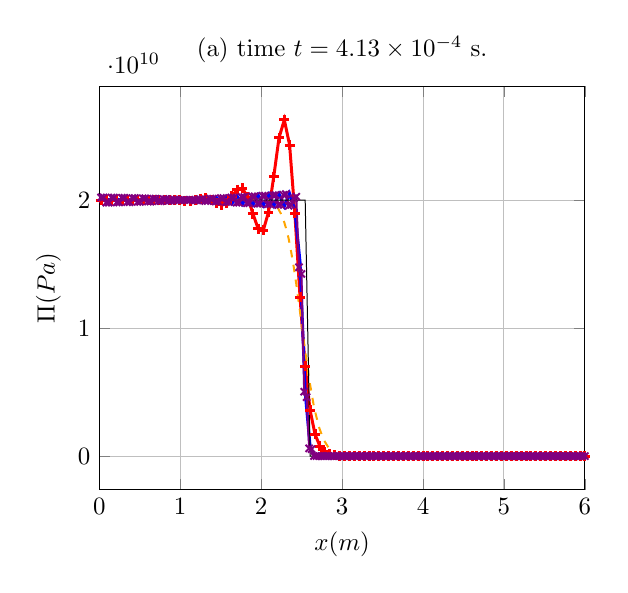
\begin{tikzpicture}[scale=0.9]
\begin{axis}[xlabel=$x (m)$,ylabel=$\Pi (Pa)$,ymajorgrids=true,xmajorgrids=true,legend pos= south west,title={(a) time $t = 4.13\times 10^{-4} $ s.},xmin=0.,xmax=6.]
\addplot[Red,very thick,mark=+,solid] coordinates {(-0.16829522461060809,20007169511.96314) (-0.10369101528636954,19993538918.151154) (-0.03910008978943477,20005752249.60066) (0.025484632606506585,19995780538.002594) (0.09006724602086946,20002982078.92515) (0.1546485608680076,19999277260.36865) (0.2192288029837782,20000480398.382977) (0.2838085169531259,20001789392.278667) (0.3483874448371409,19997301874.53342) (0.41296605184651003,20003008206.491848) (0.4775444471393354,19998613234.28465) (0.5421228879757068,20006614615.093975) (0.6067010779765869,19998205526.77761) (0.6712784021529404,19998711631.528248) (0.7358550513644272,19992106494.35627) (0.8004321132591515,20004770592.319847) (0.8650111473999984,20015779987.73382) (0.9295914037752241,20019625431.191498) (0.9941696099372187,19992929208.032467) (1.0587424231017257,19958300876.966587) (1.123311926789651,19955346446.406406) (1.1878866648233635,20018511640.579197) (1.2524750200748365,20111607980.21578) (1.3170736594252148,20136508388.211338) (1.381663458854595,20010138904.573597) (1.4462219802801475,19778030212.99804) (1.5107477640922773,19635427268.59183) (1.5752752811607438,19797599632.74197) (1.639859880303798,20289327749.506416) (1.70453378203858,20824737676.284462) (1.769262079187512,20916782028.057846) (1.8339384337847504,20225825740.178158) (1.89844144581174,18932646585.446335) (1.9627281077084087,17775081852.48631) (2.026899949421701,17642004813.115726) (2.091185400436795,19055892736.768036) (2.1558364961562164,21827268031.841457) (2.220982442003199,24860462590.307526) (2.286498524038505,26265768115.97021) (2.351967307290947,24295998059.88075) (2.4168137711136564,18956883378.505733) (2.480598163334301,12418144526.81467) (2.543246483139721,7028504053.174823) (2.604999975767945,3579770240.6871147) (2.66618758468537,1694104579.470104) (2.7270670263127124,758612765.168792) (2.7877944080472954,324010645.8165056) (2.848451732493268,132301231.12326287) (2.90907847951511,51629746.688618675) (2.969692513364221,19230481.215198454) (3.0303015063501104,6825460.685392445) (3.0909085945578147,2304741.6481061573) (3.151514997773176,739250.3468689044) (3.212121166898583,224906.37010029136) (3.2727272601131854,64808.36407273517) (3.3333333300016945,17662.648147483887) (3.3939393931074338,4546.039630207806) (3.4545454543493492,1103.2785027445323) (3.5151515151079566,252.0479295361392) (3.5757575757484754,54.104532819766206) (3.6363636363618523,10.890886483248497) (3.69696969696937,2.0511541183492015) (3.7575757575757014,0.36048087591867584) (3.81818181818181,0.05894430243048331) (3.8787878787878776,0.008907404728338756) (3.9393939393939394,0.0011956247957501686) (4.0,0.00011956247957501687) (4.0606060606060606,0.0) (4.121212121212121,0.0) (4.181818181818182,0.0) (4.242424242424242,0.0) (4.303030303030303,0.0) (4.363636363636363,0.0) (4.424242424242425,0.0) (4.484848484848485,0.0) (4.545454545454546,0.0) (4.606060606060606,0.0) (4.666666666666667,0.0) (4.7272727272727275,0.0) (4.787878787878788,0.0) (4.848484848484849,0.0) (4.909090909090909,0.0) (4.96969696969697,0.0) (5.03030303030303,0.0) (5.090909090909091,0.0) (5.151515151515151,0.0) (5.212121212121212,0.0) (5.2727272727272725,0.0) (5.333333333333334,0.0) (5.3939393939393945,0.0) (5.454545454545455,0.0) (5.515151515151516,0.0) (5.575757575757576,0.0) (5.636363636363637,0.0) (5.696969696969697,0.0) (5.757575757575758,0.0) (5.818181818181818,0.0) (5.878787878787879,0.0) (5.9393939393939394,0.0) (6.0,0.0) };
\addplot[Blue,very thick,mark=none,solid] coordinates {(-0.17172662820924992,20126286105.84016) (-0.10660603391933107,19875164406.999718) (-0.04194663943234102,20122512972.128735) (0.022732395165806486,19881553883.263596) (0.08741156754331267,20113695600.0826) (0.15209029604815277,19892923663.406227) (0.21677157984023532,20099953165.28105) (0.2814513737028933,19909115868.450443) (0.3461348221041776,20081472085.12577) (0.4108152742186133,19929906305.25904) (0.4755009353032759,20058503290.3213) (0.5401815288947392,19955007831.504406) (0.6048694507202782,20031358457.677605) (0.6695495822549338,19984074913.32308) (0.7342398618126412,20000405141.87171) (0.7989189035565396,20016709438.584362) (0.8636117080664685,19966060744.260063) (0.9282890378442423,20052467818.751507) (0.9929846146963595,19928785275.12034) (1.0576596352554701,20090869363.82577) (1.1223583072987158,19889072904.409824) (1.1870304528999478,20131405850.072147) (1.2517326020503938,19847442355.372017) (1.3164013359003341,20173552123.78648) (1.3811073800322917,19804426272.137638) (1.4457721874723826,20216777502.470745) (1.5104825561512225,19760559789.583214) (1.575142938446335,20260557805.032604) (1.6398580523466464,19716368448.944717) (1.7045135246263603,20304386827.323605) (1.769233781555915,19672356602.402267) (1.833883876574903,20347788289.080315) (1.8986096450055439,19628995435.82482) (1.96325392193934,20390327196.219734) (2.0279855406761045,19586711664.247425) (2.0926235965346587,20431618631.24346) (2.1573613774425398,19545878506.256725) (2.2219928581092483,20471336442.532116) (2.286737089006318,19506806138.044117) (2.3513616964415003,20505909410.75548) (2.416111827679838,19223361070.797165) (2.4806716443202474,15164119638.328646) (2.544309845123544,4962759374.283854) (2.605921117305293,685282540.4186183) (2.666666666666667,0.0) (2.7272727272727275,0.0) (2.787878787878788,0.0) (2.8484848484848486,0.0) (2.909090909090909,0.0) (2.9696969696969697,0.0) (3.0303030303030303,0.0) (3.090909090909091,0.0) (3.1515151515151514,0.0) (3.2121212121212124,0.0) (3.272727272727273,0.0) (3.3333333333333335,0.0) (3.393939393939394,0.0) (3.4545454545454546,0.0) (3.515151515151515,0.0) (3.5757575757575757,0.0) (3.6363636363636367,0.0) (3.6969696969696972,0.0) (3.757575757575758,0.0) (3.8181818181818183,0.0) (3.878787878787879,0.0) (3.9393939393939394,0.0) (4.0,0.0) (4.0606060606060606,0.0) (4.121212121212121,0.0) (4.181818181818182,0.0) (4.242424242424242,0.0) (4.303030303030303,0.0) (4.363636363636363,0.0) (4.424242424242425,0.0) (4.484848484848485,0.0) (4.545454545454546,0.0) (4.606060606060606,0.0) (4.666666666666667,0.0) (4.7272727272727275,0.0) (4.787878787878788,0.0) (4.848484848484849,0.0) (4.909090909090909,0.0) (4.96969696969697,0.0) (5.03030303030303,0.0) (5.090909090909091,0.0) (5.151515151515151,0.0) (5.212121212121212,0.0) (5.2727272727272725,0.0) (5.333333333333334,0.0) (5.3939393939393945,0.0) (5.454545454545455,0.0) (5.515151515151516,0.0) (5.575757575757576,0.0) (5.636363636363637,0.0) (5.696969696969697,0.0) (5.757575757575758,0.0) (5.818181818181818,0.0) (5.878787878787879,0.0) (5.9393939393939394,0.0) (6.0,0.0) };
\addplot[Orange,thick,mark=none,dashed] coordinates {(-0.17065948135616368,20000043525.826946) (-0.13846405161119207,20000131357.192825) (-0.10615855337338398,20000218494.583206) (-0.07404331926680283,20000306501.181454) (-0.04177810548697509,20000393896.47217) (-0.009673436417956368,20000482254.930782) (0.022584758948793797,20000570082.4036) (0.05468914251045678,20000658972.299118) (0.08694578874198917,20000747409.83799) (0.11905093160937343,20000837015.308666) (0.15130700223550114,20000926246.024586) (0.18341275190367462,20001016757.47824) (0.21566843234413013,20001106971.41286) (0.24777463690422233,20001198587.31625) (0.2800300115792282,20001289983.21988) (0.3121365750418777,20001382911.99803) (0.34439170296599453,20001475699.235306) (0.3764985602426821,20001570161.365646) (0.4087534845749329,20001664562.05299) (0.4408605892235251,20001760792.46614) (0.47311534282934564,20001857043.951477) (0.5052226603149179,20001955294.841774) (0.537477269066949,20002053652.623417) (0.5695847728293589,20002154196.745407) (0.6018392576971193,20002254937.886917) (0.63394692670971,20002358072.38815) (0.6662013049757795,20002461499.472862) (0.69830912223634,20002567550.322327) (0.730563408177844,20002673996.019188) (0.7626713598344566,20002783323.1565) (0.7949255653178342,20002893155.55905) (0.8270336401018328,20003006158.999344) (0.8592877752388308,20003119788.01011) (0.8913959639439372,20003236915.248775) (0.9236500375876889,20003354800.358326) (0.9557583325989031,20003476555.48888) (0.988012352597941,20003599215.36085) (1.0201207475700413,20003726170.38179) (1.0523747209384142,20003854194.74781) (1.0844832106025044,20003987003.679684) (1.1167371437039924,20004121068.23257) (1.1488457237196221,20004260484.92572) (1.1810996224233543,20004401370.18105) (1.2132082892569704,20004548271.07166) (1.2454621590450947,20004696886.54289) (1.2775709098908066,20004852300.090237) (1.309824755958588,20005009715.66264) (1.3419335886911143,20005174860.54694) (1.3741874160526513,20005342346.906036) (1.4062963291967852,20005518680.70837) (1.4385501427858645,20005697758.81623) (1.4706591355042127,20005887046.311424) (1.5029129402719827,20006079555.280518) (1.5350220123805445,20006284041.2585) (1.5672758134024902,20006492358.140556) (1.5993849654540777,20006715414.269215) (1.631638768111729,20006943437.753944) (1.6637480016793325,20007191089.639084) (1.6960018121418028,20007446834.098385) (1.7281111303121328,20007725459.210213) (1.7603649564409494,20008019319.813942) (1.7924743621157493,20008294004.40781) (1.824728211751267,20008585840.13172) (1.8568376886603435,20008554541.09674) (1.8890915456370228,20008462505.522263) (1.9212009637009544,20006730940.889435) (1.9534546670018174,20004485622.310314) (1.9855634459187166,19996264844.062057) (2.0178162660757217,19985866912.241154) (2.049922432994727,19957886954.48237) (2.0821719106575194,19923019878.742535) (2.1142699487559726,19844752482.056076) (2.146509305404184,19748673138.130287) (2.1785861511174294,19561739730.699345) (2.210799592712115,19335939752.423916) (2.24282884289106,18950316261.230713) (2.2749849883928817,18492945635.84119) (2.3069214957996795,17806784492.6505) (2.338967747836579,17010629044.48117) (2.3707479648286887,15966022841.692478) (2.4026123302922753,14785812065.51804) (2.434166526992342,13436743410.941061) (2.4657735751955867,11958066788.981596) (2.497049074903414,10483331170.150602) (2.528347122496258,8916511769.703724) (2.5593295703130683,7540569940.703419) (2.590312212342123,6120676372.669546) (2.6210295241339954,5005409973.170741) (2.651735403923134,3883807857.160711) (2.6822429663855347,3081223065.2520843) (2.712736226853065,2292253118.873356) (2.7430959078472834,1769087143.9346516) (2.773443251962098,1265410542.8025982) (2.803708355333792,951803900.811647) (2.8339646430982732,655843903.0110523) (2.864174119091245,481283905.106187) (2.894378051323549,319756521.6427987) (2.924557159507066,229045727.21750608) (2.954733115412435,146743624.4075898) (2.984896753012443,102624770.99267791) (3.015058747688463,63378554.38021657) (3.0452150104299562,43277421.13854273) (3.075370482653709,25746439.23638048) (3.105523452064602,17166812.660074137) (3.1356760689168683,9830289.851074612) (3.1658276603124804,6400759.483536921) (3.195979105635568,3525021.159262417) (3.226130156857271,2241699.5574820205) (3.2562811517774475,1186278.3528258102) (3.2864320046978017,736934.7477214294) (3.3165828374132054,374402.79637388245) (3.346733622184799,227248.07808513625) (3.3768844002016,110745.8468615504) (3.4070351630577127,65691.86429748994) (3.4371859238094924,30680.492705236302) (3.467336680073573,17790.289802416904) (3.497487435726684,7955.149116569932) (3.5276381901369445,4510.511505733829) (3.55778894438189,1929.1940661950573) (3.587939698304978,1069.8799239515781) (3.6180904521863875,437.2341897356511) (3.6482412059899048,237.23724715030917) (3.6783919597836334,92.53448438029154) (3.7085427135597566,49.13748895850961) (3.73869346733374,18.270581630057357) (3.7688442211040107,9.498103159014207) (3.7989949748738456,3.3623360506506152) (3.82914572864295,1.711835801326188) (3.859296482411972,0.5762313703130271) (3.8894472361808607,0.28742820089864735) (3.9195979899497346,0.09200332803300691) (3.9497487437185868,0.0450750547997889) (3.9798994974874353,0.013749685151127641) (4.01005025125628,0.006635717616413599) (4.040201005025126,0.0019727809129877925) (4.0703517587939695,0.0008967185968126294) (4.100502512562814,0.0003586874387250511) (4.130653266331658,0.00011956247957501691) (4.160804020100502,0.0) (4.190954773869347,0.0) (4.221105527638191,0.0) (4.251256281407035,0.0) (4.281407035175879,0.0) (4.311557788944723,0.0) (4.341708542713568,0.0) (4.371859296482412,-5.9781239787508415e-05) (4.402010050251256,0.0) (4.4321608040201,0.0) (4.4623115577889445,0.0) (4.492462311557789,0.0) (4.522613065326633,0.0) (4.552763819095477,0.0) (4.582914572864321,0.0) (4.613065326633166,0.0) (4.64321608040201,0.0) (4.673366834170854,-5.9781239787508415e-05) (4.703517587939698,0.0) (4.733668341708542,-5.9781239787508415e-05) (4.763819095477387,0.0) (4.793969849246231,0.0) (4.824120603015075,0.0) (4.8542713567839195,0.0) (4.884422110552763,0.0) (4.914572864321608,0.0) (4.944723618090452,0.0) (4.974874371859296,-5.9781239787508415e-05) (5.005025125628141,0.0) (5.035175879396984,-5.9781239787508415e-05) (5.065326633165829,0.0) (5.0954773869346734,0.0) (5.125628140703517,0.0) (5.155778894472362,0.0) (5.185929648241205,0.0) (5.21608040201005,0.0) (5.2462311557788945,0.0) (5.276381909547738,-5.9781239787508415e-05) (5.306532663316583,0.0) (5.3366834170854265,-5.9781239787508415e-05) (5.366834170854271,0.0) (5.396984924623116,0.0) (5.427135678391959,0.0) (5.457286432160804,0.0) (5.487437185929648,0.0) (5.517587939698492,0.0) (5.547738693467337,0.0) (5.57788944723618,-5.9781239787508415e-05) (5.608040201005025,0.0) (5.638190954773869,-5.9781239787508415e-05) (5.668341708542713,0.0) (5.698492462311558,0.0) (5.7286432160804015,0.0) (5.758793969849246,0.0) (5.788944723618091,0.0) (5.819095477386934,0.0) (5.849246231155779,5.978123978750844e-05) (5.879396984924623,-5.9781239787508415e-05) (5.909547738693467,0.0) (5.939698492462312,0.0) (5.969849246231155,0.0) (6.0,0.0) };
\addplot[Purple,thick,mark=x,solid] coordinates {(-0.1708904472675148,19785557608.354362) (-0.141053536291792,19785867406.07991) (-0.10639968665550317,20213101585.682953) (-0.07596722729975139,20213166639.459328) (-0.04207388662674958,19789540452.376034) (-0.011506607675021027,19789557029.70826) (0.022285105176351794,20207044209.230186) (0.052869007707743255,20207022244.274338) (0.08665834628959812,19798347997.174698) (0.1172321822636404,19798342777.723587) (0.151029412846739,20196099111.801785) (0.18158911289003257,20196061786.86517) (0.2154029118177921,19812014870.030228) (0.24594855907990398,19812000299.62603) (0.2797707639479692,20180456497.651028) (0.31030435509337834,20180413575.280464) (0.34414190966292796,19830391975.858875) (0.3746654464197197,19830363703.36432) (0.4085073802039732,20160337163.972836) (0.4390230930475627,20160297191.04402) (0.4728761360608775,19853261920.69269) (0.5033851748227214,19853214144.348965) (0.5372398018663066,20136017953.04032) (0.5677435687389828,20135992244.21921) (0.6016065301582988,19880348866.887726) (0.6321057005127878,19880275931.784782) (0.6659696058844139,20107829473.983624) (0.696465113347797,20107832721.84703) (0.7303345889699686,19911323145.714508) (0.7608267981523694,19911220393.101494) (0.794698155191189,20076150936.708942) (0.8251876402029276,20076201595.577923) (0.8590614435557611,19945806771.791153) (0.8895483774038433,19945671337.662453) (0.9234264348463641,20041403461.894547) (0.9539111397029185,20041524039.151882) (0.9877878427021151,19983380229.063835) (1.0182704154578464,19983211779.396458) (1.0521550389906216,20004041901.242966) (1.0826356465144116,20004259130.529278) (1.1165141722198928,20023590444.9662) (1.146992928994242,20023391823.879498) (1.1808842235337922,19964545222.656155) (1.2113612103069733,19964890116.037624) (1.2452405366181794,20065959588.155254) (1.2757159448575515,20065737455.962234) (1.3096140087494017,19923405655.590446) (1.340087867199397,19923913531.19163) (1.3739668745812406,20109993427.265583) (1.4044394740876944,20109759370.691113) (1.4383442989671855,19881117133.925976) (1.4688156172979114,19881828092.426723) (1.5026930749798657,20155184504.96013) (1.5331634940260768,20154958787.012196) (1.5670749872969294,19838167967.197243) (1.5975444109704615,19839129929.862263) (1.631419066113116,20201034036.189003) (1.6618879405221585,20200860914.39588) (1.695806028986006,19795048344.53005) (1.7262741487880973,19796331467.05578) (1.7601448712991692,20247083731.9241) (1.7906127153916045,20247094549.42775) (1.8245374872621891,19752175452.996067) (1.8550046971339533,19753935406.555477) (1.888870629478351,20292760865.435543) (1.9193376913168196,20293432983.43762) (1.953269542435462,19709654117.014126) (1.9837358641666532,19712407968.009735) (2.0175965864610483,20337138548.75029) (2.048062639992706,20340344997.290543) (2.082002580382462,19666867314.68073) (2.1124672812076257,19672700955.769726) (2.1463232982512577,20378078322.74046) (2.1767870343556104,20391295863.689228) (2.210737854430747,19619814494.093407) (2.241198117559328,19637708700.528072) (2.275052752024238,20408768422.209846) (2.3055096404249302,20461791611.02041) (2.339480401341693,19548900704.7548) (2.3699263513980036,19618213930.10675) (2.4037921787393377,20126713795.32762) (2.4342241255841532,20264753853.55581) (2.468186972434222,14751152292.966133) (2.4985606945703163,14228242465.12349) (2.531508975979028,5032326878.965216) (2.5617596336243342,4603536576.276086) (2.592841768880457,605310239.9535259) (2.623005846412341,539574226.1837834) (2.6532663316582914,0.0005380311580875769) (2.6834170854271355,0.0005380311580875769) (2.7135678391959797,0.0005380311580875769) (2.743718592964824,0.0004782499183000683) (2.7738693467336684,0.0005978123978750856) (2.8040201005025125,0.0005978123978750856) (2.8341708542713566,0.0005380311580875769) (2.8643216080402008,0.0005380311580875769) (2.8944723618090453,0.0005978123978750856) (2.9246231155778895,0.0005978123978750856) (2.9547738693467336,0.0004184686785125597) (2.9849246231155777,0.0003586874387250511) (3.015075376884422,0.0004782499183000683) (3.0452261306532664,0.0004184686785125597) (3.0753768844221105,0.0003586874387250511) (3.1055276381909547,0.0003586874387250511) (3.135678391959799,0.0005380311580875769) (3.165829145728643,0.0005380311580875769) (3.1959798994974875,0.0004184686785125597) (3.2261306532663316,0.0004184686785125597) (3.2562814070351758,0.0004782499183000683) (3.28643216080402,0.0004184686785125597) (3.316582914572864,0.0004782499183000683) (3.3467336683417086,0.0004184686785125597) (3.3768844221105527,0.0004184686785125597) (3.407035175879397,0.0003586874387250511) (3.437185929648241,0.0003586874387250511) (3.467336683417085,0.0003586874387250511) (3.4974874371859297,0.0003586874387250511) (3.527638190954774,0.0003586874387250511) (3.557788944723618,0.0003586874387250511) (3.587939698492462,0.0003586874387250511) (3.618090452261306,0.0003586874387250511) (3.648241206030151,0.0003586874387250511) (3.678391959798995,0.0002989061989375425) (3.708542713567839,0.0002989061989375425) (3.738693467336683,0.0004184686785125597) (3.7688442211055273,0.0004184686785125597) (3.798994974874372,0.0003586874387250511) (3.829145728643216,0.0003586874387250511) (3.85929648241206,0.0001793437193625254) (3.8894472361809043,0.0001793437193625254) (3.9195979899497484,0.0001793437193625254) (3.949748743718593,0.00011956247957501691) (3.979899497487437,0.0003586874387250511) (4.010050251256281,0.0002989061989375425) (4.040201005025126,0.0002989061989375425) (4.0703517587939695,0.0002989061989375425) (4.100502512562814,0.00023912495915003393) (4.130653266331658,0.0003586874387250511) (4.160804020100502,0.0003586874387250511) (4.190954773869347,0.0003586874387250511) (4.221105527638191,0.0003586874387250511) (4.251256281407035,0.0003586874387250511) (4.281407035175879,0.0003586874387250511) (4.311557788944723,0.0003586874387250511) (4.341708542713568,0.0002989061989375425) (4.371859296482412,0.0002989061989375425) (4.402010050251256,0.00023912495915003393) (4.4321608040201,0.00023912495915003393) (4.4623115577889445,0.00023912495915003393) (4.492462311557789,0.00023912495915003393) (4.522613065326633,0.0002989061989375425) (4.552763819095477,0.0002989061989375425) (4.582914572864321,0.0002989061989375425) (4.613065326633166,0.00023912495915003393) (4.64321608040201,0.0003586874387250511) (4.673366834170854,0.0003586874387250511) (4.703517587939698,0.0002989061989375425) (4.733668341708542,0.00023912495915003393) (4.763819095477387,0.0002989061989375425) (4.793969849246231,0.0002989061989375425) (4.824120603015075,0.0002989061989375425) (4.8542713567839195,0.0002989061989375425) (4.884422110552763,0.0003586874387250511) (4.914572864321608,0.0003586874387250511) (4.944723618090452,0.00023912495915003393) (4.974874371859296,0.00023912495915003393) (5.005025125628141,0.0003586874387250511) (5.035175879396984,0.0002989061989375425) (5.065326633165829,0.0002989061989375425) (5.0954773869346734,0.0002989061989375425) (5.125628140703517,0.00023912495915003393) (5.155778894472362,0.0002989061989375425) (5.185929648241205,0.0003586874387250511) (5.21608040201005,0.0003586874387250511) (5.2462311557788945,0.0001793437193625254) (5.276381909547738,0.0001793437193625254) (5.306532663316583,0.0002989061989375425) (5.3366834170854265,0.00023912495915003393) (5.366834170854271,0.00023912495915003393) (5.396984924623116,0.00023912495915003393) (5.427135678391959,0.00023912495915003393) (5.457286432160804,0.00023912495915003393) (5.487437185929648,0.0001793437193625254) (5.517587939698492,0.00011956247957501691) (5.547738693467337,5.978123978750844e-05) (5.57788944723618,5.978123978750844e-05) (5.608040201005025,0.0001793437193625254) (5.638190954773869,0.0001793437193625254) (5.668341708542713,0.00023912495915003393) (5.698492462311558,0.0001793437193625254) (5.7286432160804015,0.00011956247957501691) (5.758793969849246,5.978123978750844e-05) (5.788944723618091,0.00011956247957501691) (5.819095477386934,5.978123978750844e-05) (5.849246231155779,0.0) (5.879396984924623,0.0) (5.909547738693467,0.0) (5.939698492462312,5.978123978750844e-05) (5.969849246231155,-0.0001195624795750168) (6.0,0.0) };
\addplot[black,thin,mark=none,solid] coordinates {(-0.17172662820924992,19999999999.999966) (-0.10660603391933107,19999999999.999966) (-0.04194663943234102,19999999999.999966) (0.022732395165806486,19999999999.999966) (0.08741156754331267,19999999999.999966) (0.15209029604815277,19999999999.999966) (0.21677157984023532,19999999999.999966) (0.2814513737028933,19999999999.999966) (0.3461348221041776,19999999999.999966) (0.4108152742186133,19999999999.999966) (0.4755009353032759,19999999999.999966) (0.5401815288947392,19999999999.999966) (0.6048694507202782,19999999999.999966) (0.6695495822549338,19999999999.999966) (0.7342398618126412,19999999999.999966) (0.7989189035565396,19999999999.999966) (0.8636117080664685,19999999999.999966) (0.9282890378442423,19999999999.999966) (0.9929846146963595,19999999999.999966) (1.0576596352554701,19999999999.999966) (1.1223583072987158,19999999999.999966) (1.1870304528999478,19999999999.999966) (1.2517326020503938,19999999999.999966) (1.3164013359003341,19999999999.999966) (1.3811073800322917,19999999999.999966) (1.4457721874723826,19999999999.999966) (1.5104825561512225,19999999999.999966) (1.575142938446335,19999999999.999966) (1.6398580523466464,19999999999.999966) (1.7045135246263603,19999999999.999966) (1.769233781555915,19999999999.999966) (1.833883876574903,19999999999.999966) (1.8986096450055439,19999999999.999966) (1.96325392193934,19999999999.999966) (2.0279855406761045,19999999999.999966) (2.0926235965346587,19999999999.999966) (2.1573613774425398,19999999999.999966) (2.2219928581092483,19999999999.999966) (2.286737089006318,19999999999.999966) (2.3513616964415003,19999999999.999966) (2.416111827679838,19999999999.999966) (2.4806716443202474,19999999999.999966) (2.544309845123544,19999999999.999966) (2.605921117305293,0.0) (2.666666666666667,0.0) (2.7272727272727275,0.0) (2.787878787878788,0.0) (2.8484848484848486,0.0) (2.909090909090909,0.0) (2.9696969696969697,0.0) (3.0303030303030303,0.0) (3.090909090909091,0.0) (3.1515151515151514,0.0) (3.2121212121212124,0.0) (3.272727272727273,0.0) (3.3333333333333335,0.0) (3.393939393939394,0.0) (3.4545454545454546,0.0) (3.515151515151515,0.0) (3.5757575757575757,0.0) (3.6363636363636367,0.0) (3.6969696969696972,0.0) (3.757575757575758,0.0) (3.8181818181818183,0.0) (3.878787878787879,0.0) (3.9393939393939394,0.0) (4.0,0.0) (4.0606060606060606,0.0) (4.121212121212121,0.0) (4.181818181818182,0.0) (4.242424242424242,0.0) (4.303030303030303,0.0) (4.363636363636363,0.0) (4.424242424242425,0.0) (4.484848484848485,0.0) (4.545454545454546,0.0) (4.606060606060606,0.0) (4.666666666666667,0.0) (4.7272727272727275,0.0) (4.787878787878788,0.0) (4.848484848484849,0.0) (4.909090909090909,0.0) (4.96969696969697,0.0) (5.03030303030303,0.0) (5.090909090909091,0.0) (5.151515151515151,0.0) (5.212121212121212,0.0) (5.2727272727272725,0.0) (5.333333333333334,0.0) (5.3939393939393945,0.0) (5.454545454545455,0.0) (5.515151515151516,0.0) (5.575757575757576,0.0) (5.636363636363637,0.0) (5.696969696969697,0.0) (5.757575757575758,0.0) (5.818181818181818,0.0) (5.878787878787879,0.0) (5.9393939393939394,0.0) (6.0,0.0) };
%\legend{mpm,dgmpm,dgmpm 2ppc,dgmpm 2ppc (RK2),exact}
\end{axis}
\end{tikzpicture}
%%% Local Variables:
%%% mode: latex
%%% TeX-master: "../../mainManuscript"
%%% End:
}
%   {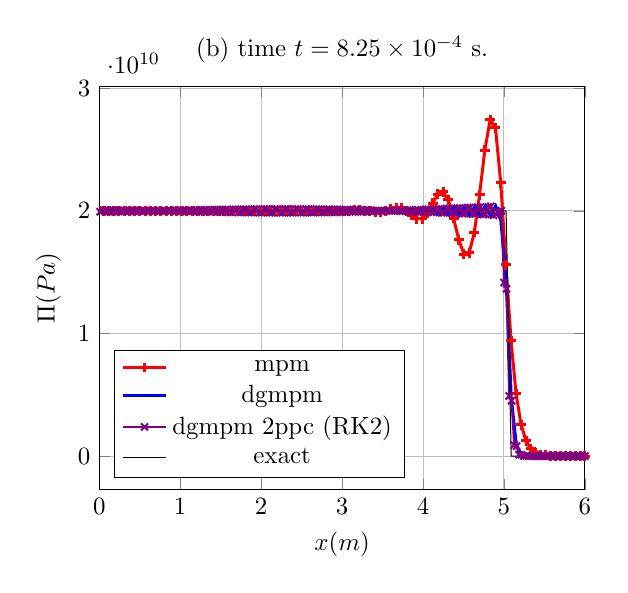
\begin{tikzpicture}[scale=0.9]
\begin{axis}[xlabel=$x (m)$,ylabel=$\Pi (Pa)$,ymajorgrids=true,xmajorgrids=true,legend pos= south west,title={(b) time $t = 8.25\times 10^{-4} $ s.},xmin=0.,xmax=6.]
\addplot[Red,very thick,mark=+,solid] coordinates {(-0.3373970335129395,20002444911.789238) (-0.2727928966297102,19997432693.913857) (-0.20820196231046736,20001959247.078884) (-0.14361740752040095,19997652072.059658) (-0.0790347885190633,20001174478.201954) (-0.014453732919982308,19998113117.396988) (0.050126384917715185,20000219977.304207) (0.1147058039394095,19998668866.378258) (0.17928462960154493,19999250601.410038) (0.24386307172432597,19999169326.347557) (0.30844111377254735,19998402881.7715) (0.3730189157030712,19999501047.64978) (0.43759644654074153,19997762967.548557) (0.50217381047918,19999609942.781967) (0.5667509959420945,19997354773.840668) (0.6313280560675543,19999501477.373802) (0.6959050053014575,19997148374.83382) (0.7604818569685504,19999225474.73323) (0.8250586461934166,19997083680.145477) (0.8896353603808954,19998851023.15548) (0.9542120453300287,19997089910.935226) (1.0187886757648426,19998440828.306694) (1.083365299089184,19997111161.46065) (1.1479418881286723,19998051169.644836) (1.2125184850646817,19997116278.583233) (1.2770950657270574,19997699692.89216) (1.3416716627444705,19997067231.472904) (1.406248258920999,19997388896.74777) (1.4708248806644153,19997000578.277737) (1.535401519422826,19997171020.844025) (1.599978191235337,19996918101.970993) (1.6645548853210443,19996920744.490818) (1.7291316080867047,19996700814.432293) (1.7937083617143608,19996691407.553604) (1.8582851678967984,19996686120.493286) (1.9228620377138623,19996772465.623905) (1.9874389634593603,19996650100.204838) (2.0520159097351134,19996304228.832874) (2.1165928542213344,19995901639.208565) (2.181169830867098,19995922422.124294) (2.245746933014004,19996569013.601753) (2.3103242301117346,19997366737.300365) (2.3749016574282744,19997253707.766594) (2.439479003437918,19995610575.776176) (2.50405608348629,19993366031.355854) (2.5686330012527394,19992897527.09602) (2.633210227393201,19996035016.03268) (2.6977882771955914,20001461417.7394) (2.7623671197745874,20004234447.067886) (2.826945847657703,19999248815.338493) (2.891523147056034,19986954084.876858) (2.9560985175931442,19976226893.658413) (3.020673338478683,19979732556.833313) (3.0852505531422554,20002734650.377262) (3.149832540815079,20033514677.442947) (3.2144183646554727,20045779859.54768) (3.279002790793957,20016543982.692215) (3.343578922732655,19949761640.288918) (3.408143766461,19886271903.166637) (3.472703046370895,19885090545.547707) (3.5372706584700393,19980762153.863453) (3.6018608542803987,20143069670.253544) (3.666476517033703,20272160418.98628) (3.731101311045297,20247014960.951336) (3.7957034722589915,20011400843.260548) (3.8602530814356824,19644164431.403908) (3.924745093767238,19352701051.419342) (3.9892134274545104,19373330976.866657) (4.0537234224180505,19827324507.865147) (4.118341053895788,20606668355.762043) (4.183090744717796,21350802856.75598) (4.247923050028822,21564506017.293846) (4.312715450250743,20887275093.29332) (4.37731903294961,19390073952.106243) (4.441637416097922,17648045449.929543) (4.505695564266106,16477972514.036726) (4.569656065119688,16564993555.823458) (4.633774257438693,18234485218.06143) (4.698311215790016,21316982189.19614) (4.763422276660747,24943663529.441895) (4.829040675663493,27423065710.3382) (4.894809718237837,26786511205.121754) (4.960153433745974,22304704037.851227) (5.024529459659876,15612866271.729282) (5.0877165905602455,9395941456.960642) (5.149868001086729,5080803829.979227) (5.211310703936358,2571948063.5769763) (5.2723407989116975,1251943821.049851) (5.333153160181875,594362859.6955562) (5.393856948062081,276921639.57925117) (5.454508383498881,126868092.89648758) (5.515135140653742,57148823.407327816) (5.575750476779182,25288021.07216049) (5.636360618733436,10978518.189306797) (5.696968440582231,4670443.034755671) (5.757575245750145,1944881.6231991085) (5.818181614449599,792440.4555923982) (5.878787799930788,317032.1081128554) (5.939393910671728,128397.83825474144) (5.9999999928647405,63394.068050559574) };
\addplot[Blue,very thick,mark=none,solid] coordinates {(-0.34300326824190164,19867161670.92257) (-0.27788319029024855,20132353190.445465) (-0.21322278871058642,19869130721.386837) (-0.14854524891661086,20129142425.138195) (-0.08386416618006085,19873652842.561867) (-0.01918775421833607,20123421266.062355) (0.04549613686190245,19880628150.922165) (0.11017305016981589,20115318727.80989) (0.17485949985090674,19889901681.750263) (0.2395368602373047,20105017064.568512) (0.30422552430806427,19901266649.63073) (0.36890325481559005,20092747885.067688) (0.43359370903377453,19914468812.52206) (0.4982717227365738,20078787280.255478) (0.5629635229582883,19929211827.51738) (0.6276417735241854,20063450128.705578) (0.6923344895943412,19945162699.15721) (0.7570129870707453,20047081201.542427) (0.8217062271247281,19961961586.06754) (0.8863850430702915,20030053095.45937) (0.9510784635094146,19979226355.574352) (1.015757722065038,20012756186.25665) (1.0804510262905567,19996560201.361286) (1.1451308857252085,19995591078.27326) (1.2098238162869241,20013559902.98507) (1.2745044463948634,19978961181.23721) (1.339196775641803,20029823630.182865) (1.40387833619713,19963265075.256836) (1.468569859873193,20044958518.655983) (1.533252484114899,19948889080.898514) (1.5979430206134242,20058587899.768158) (1.6626268056632443,19936200167.451828) (1.7273162014193637,20070358058.719982) (1.7920012052713876,19925539314.253044) (1.8566893446755617,20079944419.1636) (1.9213755875853589,19917215422.042995) (1.9860624044406507,20087057076.01931) (2.0507498716789403,19911499852.8977) (2.115435358948472,20091445622.53556) (2.1801240021419153,19908621665.315594) (2.244808217516759,20092903240.062386) (2.3094979529589694,19908763592.066013) (2.3741810192336423,20091270026.991108) (2.4388717231008803,19912058799.92498) (2.503553823894505,20086435560.409016) (2.568245325654722,19918588470.128216) (2.6329266981213357,20078340688.316597) (2.6976187741402335,19928380238.783928) (2.762299700805929,20066978548.729008) (2.826992075723227,19941407541.779408) (2.891672923066381,20052394804.467094) (2.956365346939235,19957589915.641735) (3.0210465161215225,20034687069.70895) (3.0857385707248404,19976794311.40647) (3.150420408966768,20014003488.348423) (3.2151116547381915,19998837479.325516) (3.279794587709358,19990540408.2874) (3.3444845724109693,20023489474.801964) (3.4091690555988876,19964539084.58109) (3.4738573026283968,20050478317.273846) (3.5385438113443364,19936281343.307373) (3.6032298274016155,20079495802.060196) (3.667918848609329,19906084152.544304) (3.732602130509684,20110204420.136734) (3.7972941529817468,19874293081.001152) (3.8619741937006657,20142245283.97256) (3.926669697644514,19841274680.052853) (3.9913459924348733,20175246892.79887) (4.056045440000399,19807407898.849144) (4.120717493458492,20208834504.42018) (4.185421321345374,19773074740.97144) (4.250088655916392,20242639943.665905) (4.314797270727306,19738650272.25273) (4.379459436438253,20276310806.877926) (4.44417321250515,19704493074.44567) (4.508829797148642,20309519959.73904) (4.573549076088961,19670935330.734615) (4.638199714390607,20341974420.673492) (4.702924805180256,19638273500.285717) (4.767569185544008,20373421858.440434) (4.832300363715842,19606757017.834343) (4.896938230755509,20398348853.4957) (4.961674477599282,19194568925.629593) (5.026219132132484,14312041520.443619) (5.089697845458756,4819432981.92643) (5.151288275508455,961012171.3536986) (5.212092547900456,129265691.8128923) (5.272725221999611,10032930.422299773) (5.333333333333334,0.0) (5.3939393939393945,0.0) (5.454545454545455,0.0) (5.515151515151516,0.0) (5.575757575757576,0.0) (5.636363636363637,0.0) (5.696969696969697,0.0) (5.757575757575758,0.0) (5.818181818181818,0.0) (5.878787878787879,0.0) (5.9393939393939394,0.0) (6.0,0.0) };
\addplot[Purple,thick,mark=x,solid] coordinates {(-0.3413421216005564,20084454120.70626) (-0.3115046323967783,20084503231.20538) (-0.2768503231825786,19916185104.896652) (-0.24641699137696205,19916224025.277943) (-0.21252704225382044,20082521029.067745) (-0.18195851890502224,20082494630.53035) (-0.14816447224841806,19919503737.228157) (-0.11757957066435366,19919560593.514977) (-0.08379589265784985,20077952554.12534) (-0.05322085703338879,20077898893.370735) (-0.019419148715127472,19925390458.555717) (0.011141460181846741,19925475541.195904) (0.04494772591031657,20070870972.704773) (0.07549443808768144,20070794153.22469) (0.10932301412763686,19933726420.88046) (0.13985737952332528,19933837024.581604) (0.173685926639547,20061431321.92105) (0.20421035859246994,20061332816.082695) (0.23806014963800134,19944334708.452976) (0.2685764825007371,19944466366.306778) (0.3024195284182063,20049838277.438824) (0.33292927588669197,20049719936.704403) (0.3667927137931127,19956995564.425697) (0.39729694359154255,19957143051.16299) (0.43114948448894214,20036346157.64271) (0.4616491777370185,20036210511.364494) (0.49552220217347964,19971448924.99579) (0.5260180299294327,19971606591.563793) (0.5598772972948788,20021247143.683044) (0.5903698622131245,20021097455.275764) (0.624249900829884,19987369347.34896) (0.654739595219531,19987531478.95478) (0.6886040890282352,20004870125.83432) (0.7190912475113203,20004710463.922737) (0.7529767194177145,20004410302.615177) (0.7834615704641484,20004571380.654194) (0.8173305879064932,19987574487.067276) (0.847813305881258,19987409722.84234) (0.8817031821057704,20022200269.99343) (0.9121839339935235,20022355214.726463) (0.9460571483764127,19969742299.809765) (0.9765360354593392,19969578036.0323) (1.0104294819309994,20040348503.200268) (1.040906682974281,20040492861.37563) (1.0747838335358735,19951770413.041492) (1.105259430932844,19951612839.252544) (1.1391555845596315,20058452407.676346) (1.1696298054671987,20058582471.461685) (1.2035105315252492,19934062461.007298) (1.2339834581168863,19933918134.766502) (1.26788134906568,20076105339.2744) (1.2983532590129288,20076218192.12232) (1.332237072733504,19917020987.71109) (1.3627080375199254,19916896548.399593) (1.3966066343017862,20092904393.807842) (1.4270769595734558,20092997886.904884) (1.4609633199405618,19901039886.204426) (1.4914330391974988,19900941714.78726) (1.5253313681450775,20108457966.61612) (1.5558007815742427,20108530636.852116) (1.58968921499868,19886497320.08024) (1.620158288063799,19886431164.442165) (1.6540555703547062,20122392933.588875) (1.6845245667812516,20122443880.233562) (1.7184147802161702,19873749252.240623) (1.7488835761357309,19873719842.724926) (1.7827793345331566,20134361342.940174) (1.8132481375124534,20134390084.955162) (1.8471400866548187,19863123660.159065) (1.8776086764287256,19863134343.309586) (1.9115027873522425,20144046533.93617) (1.941971308324001,20144052872.731007) (1.9758652132489007,19854915473.262917) (2.00633335571715,19854967893.19228) (2.040226079745077,20151168618.87888) (2.070693985199334,20151152531.999393) (2.104590384682496,19849382232.053566) (2.135057901533144,19849476088.127354) (2.1689496169030114,20155489277.933567) (2.199417036193448,20155450867.5519) (2.2333157795929726,19846740444.56689) (2.263782879164934,19846873351.154137) (2.29767330438176,20156815822.998478) (2.328140263166214,20156755339.15534) (2.3620411522751077,19847162606.42877) (2.392507699460935,19847330075.36992) (2.426397066000551,20155004487.461292) (2.456863380789038,20154922439.98095) (2.4907664359543715,19850774856.538464) (2.5212322666486426,19850970415.948395) (2.555120899476285,20149962895.29097) (2.585586439450331,20149860260.53971) (2.6194915665074547,19857655259.362076) (2.649956589833981,19857870713.761578) (2.6838448104013497,20141651656.730064) (2.7143095156589245,20141530176.422417) (2.7482165060193036,19867832720.558792) (2.7786806902628784,19868058547.559307) (2.8125688393803885,20130084962.0052) (2.8430326926994947,20129947521.903427) (2.8769412584352323,19881286508.15238) (2.907404596472946,19881512377.22646) (2.9412930658856,20115330328.24148) (2.9717560576395274,20115181396.04708) (3.0056658655431305,19897946940.899014) (3.036128344041352,19898162329.4085) (3.070017595121079,20097507428.18806) (3.100479700762355,20097353520.394882) (3.1343903886946634,19917696528.872005) (3.164851976527314,19917891402.385876) (3.1987425343389657,20076785327.117977) (3.2292037151467032,20076635470.893406) (3.2631148843368862,19940372025.717415) (3.29357554543851,19940537544.133724) (3.3274679679788997,20053378728.587624) (3.357928194540636,20053244881.13022) (3.3918393831412645,19965767607.411438) (3.422299107793317,19965896815.490192) (3.456193940921393,20027543050.174908) (3.486653228633958,20027440439.6467) (3.520563880585621,19993639102.67711) (3.5510227208761473,19993727568.79394) (3.5849204556914755,19999568290.3942) (3.615378895931043,19999515651.498085) (3.649288342283673,20023709203.216496) (3.6797464349135187,20023755595.7377) (3.7136474841959903,19969771717.557053) (3.744105255467703,19969791423.13771) (3.7780127218729365,20055673406.51396) (3.8084702852479175,20055680096.82016) (3.8423749893302808,19938489456.48) (3.8728323391771236,19938607645.218704) (3.906736984687898,20089205875.665604) (3.9371942857875872,20089180050.754776) (3.971102948275359,19906067025.556553) (4.001560146502916,19906314216.038258) (4.035461128102997,20123961775.83972) (4.065918424699022,20123919131.594395) (4.099831368443375,19872848196.356743) (4.130288641421362,19873262528.891777) (4.164185191417915,20159573473.009506) (4.194642662567189,20159553030.56887) (4.228560290996899,19839166473.88708) (4.259017750563116,19839808941.31075) (4.292909258187191,20195675341.985744) (4.323366935108609,20195799856.708904) (4.357289795589992,19805336038.508987) (4.387747366655722,19806358551.373158) (4.421633460585793,20231834709.36628) (4.452091150023708,20232554202.447742) (4.48602003137047,19771483196.513275) (4.516477347673006,19773429826.418495) (4.5503580637774,20267126470.97277) (4.58081526693636,20270193617.440983) (4.614751454576072,19736918846.87252) (4.645207821787056,19742059913.02803) (4.679083775444953,20298852761.491997) (4.7095395048223025,20311197166.66586) (4.743485099523246,19697906198.47693) (4.773938201390833,19716155926.428547) (4.807812253028679,20317459432.2131) (4.838261988618075,20366464115.49615) (4.872224665961511,19636335499.984386) (4.9026646932738345,19711246044.137264) (4.936550533899874,19912517877.28153) (4.966975247749498,20015432325.29268) (5.000903022698816,14157492462.311962) (5.031270011791101,13637448020.679394) (5.064107380705877,4900151134.711801) (5.094355634519364,4518545375.67135) (5.125418372928627,896010785.5143551) (5.1555887970834,812792584.0059679) (5.1859044083527275,115327096.28225213) (5.21605773200199,103644640.31290346) (5.246229541628463,7935027.787381989) (5.276380471907977,7067282.007803429) (5.306532663316583,0.0004782499183000683) (5.3366834170854265,0.0005978123978750856) (5.366834170854271,0.0004782499183000683) (5.396984924623116,0.0004782499183000683) (5.427135678391959,0.0004782499183000683) (5.457286432160804,0.0005380311580875769) (5.487437185929648,0.0005380311580875769) (5.517587939698492,0.0004782499183000683) (5.547738693467337,0.0005978123978750856) (5.57788944723618,0.0005978123978750856) (5.608040201005025,0.0005380311580875769) (5.638190954773869,0.0005380311580875769) (5.668341708542713,0.0005380311580875769) (5.698492462311558,0.0005380311580875769) (5.7286432160804015,0.0003586874387250511) (5.758793969849246,0.0002989061989375425) (5.788944723618091,0.0005380311580875769) (5.819095477386934,0.0004782499183000683) (5.849246231155779,0.0004184686785125597) (5.879396984924623,0.0004184686785125597) (5.909547738693467,0.0004782499183000683) (5.939698492462312,0.0004782499183000683) (5.969849246231155,0.0001793437193625254) (6.0,0.00023912495915003393) };
\addplot[black,thin,mark=none,solid] coordinates {(-0.34300326824190164,19999999999.999966) (-0.27788319029024855,19999999999.999966) (-0.21322278871058642,19999999999.999966) (-0.14854524891661086,19999999999.999966) (-0.08386416618006085,19999999999.999966) (-0.01918775421833607,19999999999.999966) (0.04549613686190245,19999999999.999966) (0.11017305016981589,19999999999.999966) (0.17485949985090674,19999999999.999966) (0.2395368602373047,19999999999.999966) (0.30422552430806427,19999999999.999966) (0.36890325481559005,19999999999.999966) (0.43359370903377453,19999999999.999966) (0.4982717227365738,19999999999.999966) (0.5629635229582883,19999999999.999966) (0.6276417735241854,19999999999.999966) (0.6923344895943412,19999999999.999966) (0.7570129870707453,19999999999.999966) (0.8217062271247281,19999999999.999966) (0.8863850430702915,19999999999.999966) (0.9510784635094146,19999999999.999966) (1.015757722065038,19999999999.999966) (1.0804510262905567,19999999999.999966) (1.1451308857252085,19999999999.999966) (1.2098238162869241,19999999999.999966) (1.2745044463948634,19999999999.999966) (1.339196775641803,19999999999.999966) (1.40387833619713,19999999999.999966) (1.468569859873193,19999999999.999966) (1.533252484114899,19999999999.999966) (1.5979430206134242,19999999999.999966) (1.6626268056632443,19999999999.999966) (1.7273162014193637,19999999999.999966) (1.7920012052713876,19999999999.999966) (1.8566893446755617,19999999999.999966) (1.9213755875853589,19999999999.999966) (1.9860624044406507,19999999999.999966) (2.0507498716789403,19999999999.999966) (2.115435358948472,19999999999.999966) (2.1801240021419153,19999999999.999966) (2.244808217516759,19999999999.999966) (2.3094979529589694,19999999999.999966) (2.3741810192336423,19999999999.999966) (2.4388717231008803,19999999999.999966) (2.503553823894505,19999999999.999966) (2.568245325654722,19999999999.999966) (2.6329266981213357,19999999999.999966) (2.6976187741402335,19999999999.999966) (2.762299700805929,19999999999.999966) (2.826992075723227,19999999999.999966) (2.891672923066381,19999999999.999966) (2.956365346939235,19999999999.999966) (3.0210465161215225,19999999999.999966) (3.0857385707248404,19999999999.999966) (3.150420408966768,19999999999.999966) (3.2151116547381915,19999999999.999966) (3.279794587709358,19999999999.999966) (3.3444845724109693,19999999999.999966) (3.4091690555988876,19999999999.999966) (3.4738573026283968,19999999999.999966) (3.5385438113443364,19999999999.999966) (3.6032298274016155,19999999999.999966) (3.667918848609329,19999999999.999966) (3.732602130509684,19999999999.999966) (3.7972941529817468,19999999999.999966) (3.8619741937006657,19999999999.999966) (3.926669697644514,19999999999.999966) (3.9913459924348733,19999999999.999966) (4.056045440000399,19999999999.999966) (4.120717493458492,19999999999.999966) (4.185421321345374,19999999999.999966) (4.250088655916392,19999999999.999966) (4.314797270727306,19999999999.999966) (4.379459436438253,19999999999.999966) (4.44417321250515,19999999999.999966) (4.508829797148642,19999999999.999966) (4.573549076088961,19999999999.999966) (4.638199714390607,19999999999.999966) (4.702924805180256,19999999999.999966) (4.767569185544008,19999999999.999966) (4.832300363715842,19999999999.999966) (4.896938230755509,19999999999.999966) (4.961674477599282,19999999999.999966) (5.026219132132484,19999999999.999966) (5.089697845458756,0.0) (5.151288275508455,0.0) (5.212092547900456,0.0) (5.272725221999611,0.0) (5.333333333333334,0.0) (5.3939393939393945,0.0) (5.454545454545455,0.0) (5.515151515151516,0.0) (5.575757575757576,0.0) (5.636363636363637,0.0) (5.696969696969697,0.0) (5.757575757575758,0.0) (5.818181818181818,0.0) (5.878787878787879,0.0) (5.9393939393939394,0.0) (6.0,0.0) };
\legend{mpm,dgmpm,dgmpm 2ppc (RK2),exact}
\end{axis}
\end{tikzpicture}
%%% Local Variables:
%%% mode: latex
%%% TeX-master: "../../mainManuscript"
%%% End:
}
%   \caption{shock stress $50\sigma^y$}
%   \label{fig:he_shock}
% \end{figure}
% \begin{figure}[h!]
%   \centering
%   {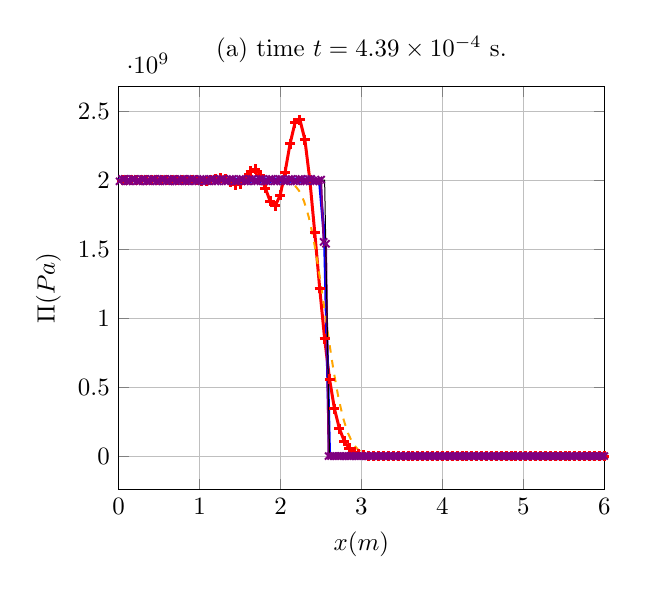
\begin{tikzpicture}[scale=0.9]
\begin{axis}[xlabel=$x (m)$,ylabel=$\Pi (Pa)$,ymajorgrids=true,xmajorgrids=true,legend pos= south west,title={(a) time $t = 4.39\times 10^{-4} $ s.},xmin=0.,xmax=6.]
\addplot[Red,very thick,mark=+,solid] coordinates {(-0.01889090575892736,2000726227.9548469) (0.04215938121847631,1999333692.2170322) (0.10320950300088187,2000564307.210718) (0.1642595721497595,1999551619.5161746) (0.22530959528412595,2000366086.7014122) (0.2863596365377364,1999918681.081198) (0.34740962154368255,1999967513.1983385) (0.4084596019243027,1999982956.3759255) (0.4695095542813397,1999789300.767052) (0.5305595706356425,2000638143.0446692) (0.5916096101001108,2000058185.8142667) (0.6526595840065709,2000089500.8199706) (0.7137094080712463,1998731982.696904) (0.7747591964204517,1999802718.761434) (0.8358092400792819,2001103352.5160503) (0.8968596075653851,2002797653.0377228) (0.9579099107745452,2000545034.2858593) (1.0189595027783396,1996318945.1727874) (1.0800083591701581,1993841183.3513687) (1.1410574970379839,1998917122.885443) (1.2021083083094746,2009171450.4722426) (1.2631608670075336,2014924382.2673836) (1.324213039463032,2005656899.5451016) (1.385261769152474,1983449039.423849) (1.4463061626617941,1966015537.327388) (1.507349635271763,1975043578.4303389) (1.5683984989928055,2015342835.6991093) (1.6294570537824011,2063738687.704247) (1.6905226695860884,2079996363.0337298) (1.7515852284367635,2035769364.3281224) (1.8126325838500514,1940918000.2995517) (1.8736591534269504,1845811486.1301281) (1.9346719362907874,1815039899.0369656) (1.9956894703716108,1889210362.9092839) (2.0567336535453324,2058642788.6612728) (2.117818634233786,2262898814.531011) (2.178942416069636,2414862117.653746) (2.240085148148831,2437155605.434466) (2.301214705448431,2293758990.699916) (2.3622968082809916,2001786574.9585006) (2.4233050712621194,1618923825.3431814) (2.4842269247483553,1216053195.9451652) (2.5450639204752132,851463994.3153192) (2.605827780198291,557925039.8409315) (2.66653493894023,343357124.31856114) (2.7272019233986486,199050644.20604298) (2.7878426090238304,108945510.80319592) (2.8484672666547697,56388618.61462657) (2.9090827809076343,27631268.92148142) (2.9696933946574,12828198.479249047) (3.030301534387653,5645398.76980634) (3.0909084955126,2355626.776140429) (3.15151492615744,932070.1392538762) (3.212121131032279,349709.3400203979) (3.2727272450009446,124397.82639027077) (3.333333324329144,41941.30302034219) (3.3939393911637925,13397.315005244573) (3.4545454537338864,4052.370067713768) (3.515151514926613,1159.9211676619566) (3.5757575756985602,313.92767018390856) (3.6363636363489893,80.26085778895391) (3.6969696969662627,19.36314356717398) (3.7575757575749984,4.402469841671484) (3.8181818181816607,0.9419729953317703) (3.878787878787848,0.1893869676468267) (3.9393939393939337,0.03568940015314253) (3.999999999999999,0.006277030177688385) (4.0606060606060606,0.0010162810763876433) (4.121212121212121,0.00011956247957501687) (4.181818181818182,0.0) (4.242424242424242,0.0) (4.303030303030303,0.0) (4.363636363636363,0.0) (4.424242424242425,0.0) (4.484848484848485,0.0) (4.545454545454546,0.0) (4.606060606060606,0.0) (4.666666666666667,0.0) (4.7272727272727275,0.0) (4.787878787878788,0.0) (4.848484848484849,0.0) (4.909090909090909,0.0) (4.96969696969697,0.0) (5.03030303030303,0.0) (5.090909090909091,0.0) (5.151515151515151,0.0) (5.212121212121212,0.0) (5.2727272727272725,0.0) (5.333333333333334,0.0) (5.3939393939393945,0.0) (5.454545454545455,0.0) (5.515151515151516,0.0) (5.575757575757576,0.0) (5.636363636363637,0.0) (5.696969696969697,0.0) (5.757575757575758,0.0) (5.818181818181818,0.0) (5.878787878787879,0.0) (5.9393939393939394,0.0) (6.0,0.0) };
\addplot[Blue,very thick,mark=none,solid] coordinates {(-0.01905005116856936,2008739016.0347507) (0.04200625800028209,1991261736.4427555) (0.10305754928183601,2008739100.409834) (0.16410893267859902,1991261521.605884) (0.22516022487211998,2008739334.4376273) (0.28621163420310985,1991261157.0218182) (0.3472629006887729,2008739718.3484042) (0.40831433629779745,1991260642.4918854) (0.4693655770844152,2008740252.4789007) (0.5304170389659988,1991259977.710147) (0.591468254064157,2008740937.273132) (0.6525197422102871,1991259162.2632153) (0.713570931632428,2008741773.281487) (0.7746224460325223,1991258195.6316195) (0.8356736097927291,2008742761.1610267) (0.8967251504336042,1991257077.1895308) (0.9577762885477589,2008743901.6730618) (1.0188278554137018,1991255806.2060382) (1.0798789678994447,2008745195.6865165) (1.1409305609721991,1991254381.844086) (1.2019816478489238,2008746644.1731992) (1.2630332671077074,1991252803.1625357) (1.3240843283965613,2008748248.2084675) (1.3851359738180737,1991251069.1156514) (1.4461870095419576,2008750008.9730506) (1.5072386811003957,1991249178.5552225) (1.5682896912839626,2008751927.748467) (1.6293413889510406,1991247130.2292893) (1.690392373620723,2008754005.9189367) (1.7514440973658394,1991244922.7847517) (1.812495056549925,2008756244.9680448) (1.8735468063397946,1991242554.768552) (1.9345977400681083,2008758646.4805305) (1.995649515867116,1991240024.626371) (2.0567004241713285,2008761212.1386473) (2.117752225941453,1991237330.7058423) (2.178803108854988,2008763943.7223768) (2.23985493655583,1991234471.2575831) (2.30090579411386,2008766843.192291) (2.3619576477026816,1991231443.3554277) (2.423008479941872,2008763352.9954166) (2.484060357772498,1983892732.551015) (2.5451094294578325,1563462712.6817071) (2.606060606060606,0.0) (2.666666666666667,0.0) (2.7272727272727275,0.0) (2.787878787878788,0.0) (2.8484848484848486,0.0) (2.909090909090909,0.0) (2.9696969696969697,0.0) (3.0303030303030303,0.0) (3.090909090909091,0.0) (3.1515151515151514,0.0) (3.2121212121212124,0.0) (3.272727272727273,0.0) (3.3333333333333335,0.0) (3.393939393939394,0.0) (3.4545454545454546,0.0) (3.515151515151515,0.0) (3.5757575757575757,0.0) (3.6363636363636367,0.0) (3.6969696969696972,0.0) (3.757575757575758,0.0) (3.8181818181818183,0.0) (3.878787878787879,0.0) (3.9393939393939394,0.0) (4.0,0.0) (4.0606060606060606,0.0) (4.121212121212121,0.0) (4.181818181818182,0.0) (4.242424242424242,0.0) (4.303030303030303,0.0) (4.363636363636363,0.0) (4.424242424242425,0.0) (4.484848484848485,0.0) (4.545454545454546,0.0) (4.606060606060606,0.0) (4.666666666666667,0.0) (4.7272727272727275,0.0) (4.787878787878788,0.0) (4.848484848484849,0.0) (4.909090909090909,0.0) (4.96969696969697,0.0) (5.03030303030303,0.0) (5.090909090909091,0.0) (5.151515151515151,0.0) (5.212121212121212,0.0) (5.2727272727272725,0.0) (5.333333333333334,0.0) (5.3939393939393945,0.0) (5.454545454545455,0.0) (5.515151515151516,0.0) (5.575757575757576,0.0) (5.636363636363637,0.0) (5.696969696969697,0.0) (5.757575757575758,0.0) (5.818181818181818,0.0) (5.878787878787879,0.0) (5.9393939393939394,0.0) (6.0,0.0) };
\addplot[Orange,thick,mark=none,dashed] coordinates {(-0.01889946980668934,2000000476.6320922) (0.011472982262261672,2000001438.4851248) (0.04184684081405173,2000002392.7012472) (0.07221830818119625,2000003356.4999018) (0.1025917130426491,2000004313.5796762) (0.13296300523969845,2000005281.2865465) (0.16333630052391546,2000006243.1661801) (0.19370758569637742,2000007216.7782526) (0.22408085754430615,2000008185.4363225) (0.2544521532603863,2000009167.002689) (0.28482541656310756,2000010144.4770656) (0.3151967209063114,2000011136.1183035) (0.3455699783645009,2000012124.525834) (0.375941289271186,2000013128.4548132) (0.4063145421596361,2000014130.011946) (0.4366858582807102,2000015148.5565734) (0.46705910748905927,2000016165.6025586) (0.49743042788464853,2000017201.230468) (0.5278036740577438,2000018236.2531688) (0.5581749980487619,2000019291.6008966) (0.5885482416749542,2000020347.2658136) (0.6189195687537644,2000021425.1713114) (0.6492928102146956,2000022504.3554904) (0.6796641399908071,2000023607.8955212) (0.7100373795927971,2000024713.7263746) (0.7404087117584984,2000025846.261096) (0.770781949752748,2000026982.1621099) (0.801153284060668,2000028147.3869371) (0.8315265206562344,2000029317.1320484) (0.8618978569046679,2000030519.139193) (0.8922710922772454,2000031726.917393) (0.9226424303005011,2000032970.2716842) (0.9530156645993644,2000034220.765175) (0.9833870042609338,2000035510.5942588) (1.0137602376150086,2000036809.0741432) (1.0441315788021248,2000038151.1810029) (1.0745048113249476,2000039503.6248093) (1.1048761539440453,2000040904.6263094) (1.135249385737295,2000042317.864904) (1.1656207297105001,2000043785.3669105) (1.1959939608663954,2000045267.2687786) (1.2263653061291135,2000046810.0885317) (1.256738536732258,2000048369.7969508) (1.287109883231583,2000049998.2522519) (1.317483113360697,2000051646.4962869) (1.3478544610543197,2000053372.763049) (1.3782276907838837,2000055122.2291121) (1.4085990396392938,2000056960.6600883) (1.4389722690410596,2000058826.1717622) (1.4693436190349667,2000060793.545488) (1.4997168481792058,2000062791.8230162) (1.5300881992973736,2000064911.2737882) (1.560461428254117,2000067066.273204) (1.5908327804937845,2000069397.197215) (1.6212060093376797,2000071787.9900625) (1.6515773627224224,2000074524.9349527) (1.6819505915575537,2000077452.350958) (1.7123219461747121,2000080903.035157) (1.7426951752003998,2000084936.5086977) (1.7730665311339828,2000087540.9977086) (1.803439760589524,2000090978.4911919) (1.8338111168181779,2000077477.0261457) (1.8641843455780502,2000060918.7151618) (1.89455569411346,1999958154.3051436) (1.9249289121352766,1999828194.6022284) (1.9553002169004803,1999383368.9065702) (1.9856733785402865,1998822980.5573165) (2.016044517032017,1997345314.8488786) (2.0464174695217108,1995510656.7783453) (2.076788104100392,1991451764.8388326) (2.1071604354370703,1986509217.5580401) (2.137529784396641,1976980528.1385503) (2.167900564514874,1965628394.4283447) (2.198267080236323,1946149393.6631432) (2.2286345177754954,1923474337.231913) (2.258995557200682,1888386109.4679742) (2.2893566818194317,1848505164.4681375) (2.319708344599485,1792363112.5595503) (2.3500589114299957,1730086099.196376) (2.3803962543095176,1649845080.7546284) (2.410731075812863,1562996199.566734) (2.441048815997596,1460110948.707434) (2.4713625925459266,1351464850.755648) (2.501656185567081,1232676868.5027761) (2.531944653047198,1110279637.2963586) (2.5622113868239693,986331460.2560489) (2.5924723706106327,861678218.7179918) (2.6227120342555033,744346670.210031) (2.652945972784969,629124816.8222382) (2.6831608274884244,527964164.37957025) (2.71337055903147,430909155.97551006) (2.743564662850764,351163528.32019114) (2.7737546123498764,276374743.51695853) (2.8039328190674553,218694935.4413843) (2.8341079548422545,165789527.4489097) (2.8642749709886175,127396775.37849465) (2.8944399082519543,92940066.64930406) (2.9245996662205296,69367708.39847162) (2.9547581309384414,48658784.39870716) (2.9849135418650325,35284991.624521784) (3.015068211540017,23779444.403994165) (3.045221214363269,16758966.548834514) (3.075373824972491,10842273.254041858) (3.1055255924007317,7429200.53377867) (3.1356771679720667,4610317.903746986) (3.165828347947403,3072574.7950721933) (3.195979441069561,1827504.9990729818) (3.2261303619529405,1185127.147576748) (3.2562812464212003,675046.6861063467) (3.2864320612710896,426155.42986476084) (3.3165828619726887,232265.35139310345) (3.346733636544425,142805.4142200062) (3.3768844060203573,74409.37325305404) (3.407035166388237,44577.386497880674) (3.4371859250543553,22185.129789297524) (3.4673366807720183,12956.171896078795) (3.4974874359627095,6152.611330358401) (3.52763819026706,3504.3041958899166) (3.557788944420106,1586.2018885915058) (3.587939698325784,881.5070838911788) (3.618090452191194,379.88885595171956) (3.6482412059925275,206.08344960854643) (3.678391959783931,84.45086513091069) (3.7085427135599374,44.74051898936539) (3.738693467333677,17.410030683202127) (3.7688442211039845,9.011483867110433) (3.798994974873815,3.3249727757824945) (3.8291457286429367,1.6822440876309985) (3.8592964824119647,0.5877093683522783) (3.889447236180857,0.2908357315665427) (3.9195979899497333,0.09612823357834788) (3.9497487437185854,0.04662936703426465) (3.979899497487435,0.014706184987727878) (4.01005025125628,0.0069944050551386675) (4.040201005025126,0.0021521246323503206) (4.0703517587939695,0.001016281076387647) (4.100502512562814,0.0003586874387250511) (4.130653266331658,0.00011956247957501691) (4.160804020100502,5.978123978750844e-05) (4.190954773869347,0.0) (4.221105527638191,0.0) (4.251256281407035,0.0) (4.281407035175879,0.0) (4.311557788944723,0.0) (4.341708542713568,0.0) (4.371859296482412,-5.9781239787508415e-05) (4.402010050251256,0.0) (4.4321608040201,0.0) (4.4623115577889445,0.0) (4.492462311557789,0.0) (4.522613065326633,0.0) (4.552763819095477,0.0) (4.582914572864321,0.0) (4.613065326633166,0.0) (4.64321608040201,0.0) (4.673366834170854,-5.9781239787508415e-05) (4.703517587939698,0.0) (4.733668341708542,0.0) (4.763819095477387,0.0) (4.793969849246231,0.0) (4.824120603015075,0.0) (4.8542713567839195,0.0) (4.884422110552763,0.0) (4.914572864321608,0.0) (4.944723618090452,0.0) (4.974874371859296,0.0) (5.005025125628141,0.0) (5.035175879396984,0.0) (5.065326633165829,0.0) (5.0954773869346734,0.0) (5.125628140703517,0.0) (5.155778894472362,0.0) (5.185929648241205,0.0) (5.21608040201005,0.0) (5.2462311557788945,0.0) (5.276381909547738,-5.9781239787508415e-05) (5.306532663316583,0.0) (5.3366834170854265,-5.9781239787508415e-05) (5.366834170854271,0.0) (5.396984924623116,0.0) (5.427135678391959,0.0) (5.457286432160804,0.0) (5.487437185929648,0.0) (5.517587939698492,0.0) (5.547738693467337,0.0) (5.57788944723618,0.0) (5.608040201005025,5.978123978750844e-05) (5.638190954773869,-5.9781239787508415e-05) (5.668341708542713,0.0) (5.698492462311558,0.0) (5.7286432160804015,0.0) (5.758793969849246,0.0) (5.788944723618091,0.0) (5.819095477386934,-5.9781239787508415e-05) (5.849246231155779,5.978123978750844e-05) (5.879396984924623,0.0) (5.909547738693467,0.0) (5.939698492462312,0.0) (5.969849246231155,0.0) (6.0,0.0) };
\addplot[Purple,thick,mark=x,solid] coordinates {(-0.018953461066473463,1991446661.061328) (0.011194714201811728,1991447340.1765282) (0.04179263124474906,2008553616.6801457) (0.07194754383908661,2008553786.3057418) (0.10253643380986284,1991447493.3310626) (0.13269301032617906,1991447574.3422425) (0.16328078147576108,2008554572.7002) (0.19343774764936655,2008554582.1389053) (0.2240253779425685,1991447859.6478121) (0.25418241511482015,1991447930.5818691) (0.28476989626688765,2008555624.9177055) (0.3149269257596361,2008555623.2558448) (0.3455145674347823,1991448034.9819658) (0.3756715692879528,1991448133.6042144) (0.4062590714943057,2008556842.0924373) (0.4364160416359035,2008556838.9115138) (0.467003771159221,1991448037.4972131) (0.49716070825940945,1991448166.2255507) (0.527748249418257,2008558224.400137) (0.5579051540553267,2008558220.3215702) (0.5884929746851078,1991447868.2226775) (0.6186498466884454,1991448027.2040389) (0.6492374264275679,2008559771.3514504) (0.6793942666629291,2008559766.4251652) (0.7099821771011725,1991447527.543242) (0.7401389854675806,1991447716.7777178) (0.7707266022892127,2008561486.8090549) (0.8008833796675556,2008561481.0619845) (0.8314713783415424,1991447015.2910771) (0.8616281246321296,1991447234.7695084) (0.8922157769826508,2008563372.0888019) (0.922372493064097,2008563365.5949845) (0.9529605783946749,1991446329.7058122) (0.9831172641638408,1991446579.4234667) (1.013704950502113,2008565427.774235) (1.043861606833815,2008565420.8015227) (1.0744497772541894,1991445469.688907) (1.1046064040410184,1991445749.669622) (1.1351941228445261,2008567654.0964527) (1.1653507209569671,2008567647.6765823) (1.195938974915969,1991444434.1637495) (1.2260955442415553,1991444744.559402) (1.2566832940090453,2008570050.2893353) (1.286839835413446,2008570048.467054) (1.3174281713785905,1991443221.7297113) (1.3475846847426682,1991443563.2392223) (1.3781724639980146,2008572611.4914522) (1.4083289501820841,2008572630.206443) (1.4389173666457995,1991441829.765011) (1.469073825519406,1991442205.4102721) (1.4996616328369274,2008575316.3861573) (1.5298180652886002,2008575418.546248) (1.5604065608948054,1991440250.8294203) (1.5905629670328438,1991440673.458793) (1.6211508009003384,2008578078.4761584) (1.651307181902967,2008578512.435198) (1.6818957543055844,1991438457.6398063) (1.7120521100573114,1991438981.576465) (1.7426399679238898,2008580553.9702086) (1.7727962994057174,2008582300.2559524) (1.8033849467032101,1991436340.3404675) (1.833541253464869,1991437194.6760008) (1.8641291340288655,2008581384.4771564) (1.8942854172504617,2008588314.2161562) (1.9248741386090946,1991433444.741186) (1.9550303967770726,1991435593.872973) (1.985618299764926,2008575211.952947) (2.0157745348986764,2008602607.6126542) (2.046363331872024,1991427881.1583545) (2.0765195383045882,1991435378.6636598) (2.1071074672449113,2008540913.448154) (2.1372636502512763,2008649104.02732) (2.167852533779668,1991411780.894133) (2.198008671382919,1991441640.7525687) (2.228596644878877,2008395232.284703) (2.258752754918473,2008822359.8198197) (2.289341773203813,1991352408.047383) (2.3194977696318317,1991475946.8571541) (2.350085866291964,2007809494.577574) (2.3802418153253666,2009495560.7708085) (2.41083116453372,1991111400.0449364) (2.440986728457478,1991626928.107113) (2.471575265426608,1997987384.3139741) (2.5017306963085564,2003928221.7149866) (2.5323193981554217,1552508599.2255695) (2.5624732054671786,1538607374.1694043) (2.5929648241206027,0.000717374877450103) (2.6231155778894473,0.0006575936376625943) (2.6532663316582914,0.0003586874387250511) (2.6834170854271355,0.0003586874387250511) (2.7135678391959797,0.0006575936376625943) (2.743718592964824,0.0006575936376625943) (2.7738693467336684,0.0005978123978750856) (2.8040201005025125,0.0005978123978750856) (2.8341708542713566,0.0005380311580875769) (2.8643216080402008,0.0004782499183000683) (2.8944723618090453,0.00023912495915003393) (2.9246231155778895,0.00023912495915003393) (2.9547738693467336,0.0005380311580875769) (2.9849246231155777,0.0005380311580875769) (3.015075376884422,0.0001793437193625254) (3.0452261306532664,0.0001793437193625254) (3.0753768844221105,0.0005978123978750856) (3.1055276381909547,0.0005380311580875769) (3.135678391959799,0.00023912495915003393) (3.165829145728643,0.00023912495915003393) (3.1959798994974875,0.0004782499183000683) (3.2261306532663316,0.0004184686785125597) (3.2562814070351758,0.0004782499183000683) (3.28643216080402,0.0004782499183000683) (3.316582914572864,5.978123978750844e-05) (3.3467336683417086,0.0) (3.3768844221105527,0.0005978123978750856) (3.407035175879397,0.0005380311580875769) (3.437185929648241,0.00023912495915003393) (3.467336683417085,0.0001793437193625254) (3.4974874371859297,0.0005380311580875769) (3.527638190954774,0.0005380311580875769) (3.557788944723618,0.0005380311580875769) (3.587939698492462,0.0005380311580875769) (3.618090452261306,5.978123978750844e-05) (3.648241206030151,0.00011956247957501691) (3.678391959798995,0.0004782499183000683) (3.708542713567839,0.0004782499183000683) (3.738693467336683,-0.00029890619893754183) (3.7688442211055273,-0.00029890619893754183) (3.798994974874372,0.0005978123978750856) (3.829145728643216,0.0005978123978750856) (3.85929648241206,0.0001793437193625254) (3.8894472361809043,0.00011956247957501691) (3.9195979899497484,0.0001793437193625254) (3.949748743718593,0.00011956247957501691) (3.979899497487437,0.0004184686785125597) (4.010050251256281,0.0004184686785125597) (4.040201005025126,0.0) (4.0703517587939695,-0.0001195624795750168) (4.100502512562814,0.0006575936376625943) (4.130653266331658,0.0005978123978750856) (4.160804020100502,0.0) (4.190954773869347,0.0) (4.221105527638191,0.0002989061989375425) (4.251256281407035,0.00023912495915003393) (4.281407035175879,0.00023912495915003393) (4.311557788944723,0.0001793437193625254) (4.341708542713568,0.0002989061989375425) (4.371859296482412,0.0002989061989375425) (4.402010050251256,-5.9781239787508415e-05) (4.4321608040201,-5.9781239787508415e-05) (4.4623115577889445,0.0006575936376625943) (4.492462311557789,0.0006575936376625943) (4.522613065326633,-0.00032879681883129597) (4.552763819095477,-0.00032879681883129597) (4.582914572864321,0.0008369373570251206) (4.613065326633166,0.0007771561172376117) (4.64321608040201,0.0) (4.673366834170854,-5.9781239787508415e-05) (4.703517587939698,0.0003586874387250511) (4.733668341708542,0.0002989061989375425) (4.763819095477387,-0.00032879681883129597) (4.793969849246231,-0.00029890619893754183) (4.824120603015075,0.0004184686785125597) (4.8542713567839195,0.0003586874387250511) (4.884422110552763,0.0003586874387250511) (4.914572864321608,0.0003586874387250511) (4.944723618090452,0.0004782499183000683) (4.974874371859296,0.0004184686785125597) (5.005025125628141,-0.0001195624795750168) (5.035175879396984,-0.0001195624795750168) (5.065326633165829,0.0005978123978750856) (5.0954773869346734,0.0005978123978750856) (5.125628140703517,0.0) (5.155778894472362,5.978123978750844e-05) (5.185929648241205,0.0006575936376625943) (5.21608040201005,0.0005978123978750856) (5.2462311557788945,-0.00029890619893754183) (5.276381909547738,-0.00029890619893754183) (5.306532663316583,5.978123978750844e-05) (5.3366834170854265,5.978123978750844e-05) (5.366834170854271,0.0002989061989375425) (5.396984924623116,0.00023912495915003393) (5.427135678391959,0.0) (5.457286432160804,-5.9781239787508415e-05) (5.487437185929648,-0.00017934371936252516) (5.517587939698492,-0.00017934371936252516) (5.547738693467337,0.0005978123978750856) (5.57788944723618,0.0005380311580875769) (5.608040201005025,0.0003586874387250511) (5.638190954773869,0.0002989061989375425) (5.668341708542713,-0.00032879681883129597) (5.698492462311558,-0.00032879681883129597) (5.7286432160804015,0.0004782499183000683) (5.758793969849246,0.0004782499183000683) (5.788944723618091,-0.0003885780586188042) (5.819095477386934,-0.0003885780586188042) (5.849246231155779,0.0005978123978750856) (5.879396984924623,0.0005978123978750856) (5.909547738693467,-0.0002391249591500335) (5.939698492462312,-0.0002391249591500335) (5.969849246231155,0.0) (6.0,0.0001793437193625254) };
\addplot[black,thin,mark=none,solid] coordinates {(-0.01905005116856936,2000000000.0000362) (0.04200625800028209,2000000000.0000362) (0.10305754928183601,2000000000.0000362) (0.16410893267859902,2000000000.0000362) (0.22516022487211998,2000000000.0000362) (0.28621163420310985,2000000000.0000362) (0.3472629006887729,2000000000.0000362) (0.40831433629779745,2000000000.0000362) (0.4693655770844152,2000000000.0000362) (0.5304170389659988,2000000000.0000362) (0.591468254064157,2000000000.0000362) (0.6525197422102871,2000000000.0000362) (0.713570931632428,2000000000.0000362) (0.7746224460325223,2000000000.0000362) (0.8356736097927291,2000000000.0000362) (0.8967251504336042,2000000000.0000362) (0.9577762885477589,2000000000.0000362) (1.0188278554137018,2000000000.0000362) (1.0798789678994447,2000000000.0000362) (1.1409305609721991,2000000000.0000362) (1.2019816478489238,2000000000.0000362) (1.2630332671077074,2000000000.0000362) (1.3240843283965613,2000000000.0000362) (1.3851359738180737,2000000000.0000362) (1.4461870095419576,2000000000.0000362) (1.5072386811003957,2000000000.0000362) (1.5682896912839626,2000000000.0000362) (1.6293413889510406,2000000000.0000362) (1.690392373620723,2000000000.0000362) (1.7514440973658394,2000000000.0000362) (1.812495056549925,2000000000.0000362) (1.8735468063397946,2000000000.0000362) (1.9345977400681083,2000000000.0000362) (1.995649515867116,2000000000.0000362) (2.0567004241713285,2000000000.0000362) (2.117752225941453,2000000000.0000362) (2.178803108854988,2000000000.0000362) (2.23985493655583,2000000000.0000362) (2.30090579411386,2000000000.0000362) (2.3619576477026816,2000000000.0000362) (2.423008479941872,2000000000.0000362) (2.484060357772498,2000000000.0000362) (2.5451094294578325,2000000000.0000362) (2.606060606060606,0.0) (2.666666666666667,0.0) (2.7272727272727275,0.0) (2.787878787878788,0.0) (2.8484848484848486,0.0) (2.909090909090909,0.0) (2.9696969696969697,0.0) (3.0303030303030303,0.0) (3.090909090909091,0.0) (3.1515151515151514,0.0) (3.2121212121212124,0.0) (3.272727272727273,0.0) (3.3333333333333335,0.0) (3.393939393939394,0.0) (3.4545454545454546,0.0) (3.515151515151515,0.0) (3.5757575757575757,0.0) (3.6363636363636367,0.0) (3.6969696969696972,0.0) (3.757575757575758,0.0) (3.8181818181818183,0.0) (3.878787878787879,0.0) (3.9393939393939394,0.0) (4.0,0.0) (4.0606060606060606,0.0) (4.121212121212121,0.0) (4.181818181818182,0.0) (4.242424242424242,0.0) (4.303030303030303,0.0) (4.363636363636363,0.0) (4.424242424242425,0.0) (4.484848484848485,0.0) (4.545454545454546,0.0) (4.606060606060606,0.0) (4.666666666666667,0.0) (4.7272727272727275,0.0) (4.787878787878788,0.0) (4.848484848484849,0.0) (4.909090909090909,0.0) (4.96969696969697,0.0) (5.03030303030303,0.0) (5.090909090909091,0.0) (5.151515151515151,0.0) (5.212121212121212,0.0) (5.2727272727272725,0.0) (5.333333333333334,0.0) (5.3939393939393945,0.0) (5.454545454545455,0.0) (5.515151515151516,0.0) (5.575757575757576,0.0) (5.636363636363637,0.0) (5.696969696969697,0.0) (5.757575757575758,0.0) (5.818181818181818,0.0) (5.878787878787879,0.0) (5.9393939393939394,0.0) (6.0,0.0) };
%\legend{mpm,dgmpm,dgmpm 2ppc,dgmpm 2ppc (RK2),exact}
\end{axis}
\end{tikzpicture}
%%% Local Variables:
%%% mode: latex
%%% TeX-master: "../../mainManuscript"
%%% End:
}
%   {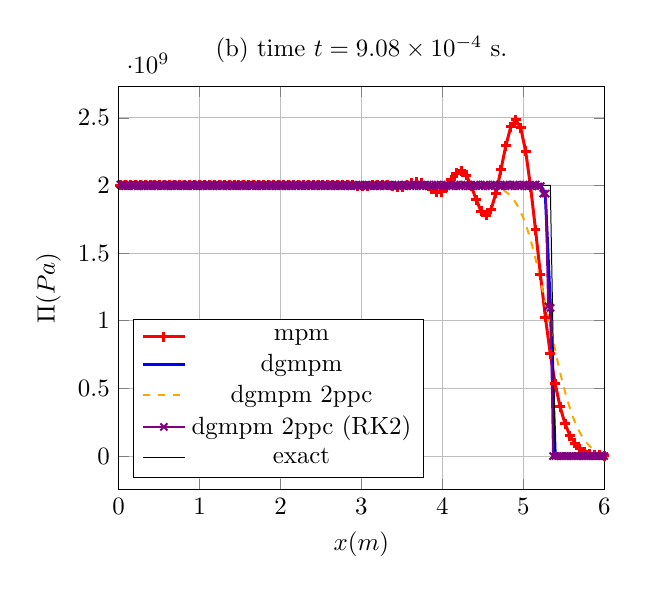
\begin{tikzpicture}[scale=0.9]
\begin{axis}[xlabel=$x (m)$,ylabel=$\Pi (Pa)$,ymajorgrids=true,xmajorgrids=true,legend pos= south west,title={(b) time $t = 9.08\times 10^{-4} $ s.},xmin=0.,xmax=6.]
\addplot[Red,very thick,mark=+,solid] coordinates {(-0.03923052052922343,2000240481.1233327) (0.021819761015892163,1999769738.8663158) (0.0828698927161351,2000218983.1347811) (0.1439199523557292,1999809950.54204) (0.20496998238621425,2000170838.6984289) (0.266019997207666,1999872129.80287) (0.32706999231126516,2000106436.8640933) (0.38811998365041567,1999944280.2454906) (0.449169959029736,2000038581.9512253) (0.510219934372632,2000013690.4345057) (0.5712698969291694,1999979089.5826085) (0.6323198600631447,2000070050.8467832) (0.6933698136476303,1999936253.3022394) (0.7544197669696648,2000107588.3199086) (0.8154697138768967,1999913395.649439) (0.876519659147888,2000125156.8768682) (0.9375696007168677,1999909211.6999958) (0.9986195394150338,2000126157.9927893) (1.059669476515721,1999919755.674749) (1.1207194099155477,2000115626.1187456) (1.1817693429480685,1999938103.4741611) (1.2428192719189772,2000098747.9520392) (1.3038692012782542,1999960657.9597352) (1.3649191269853391,2000083196.644746) (1.4259690532702223,1999982772.5176466) (1.4870189759372838,2000065998.3151865) (1.548068898510965,1999996968.6891499) (1.6091188183068375,2000054865.2647946) (1.670168739008601,2000018826.7281826) (1.731218658453022,2000056284.8743527) (1.7922685772512423,2000025238.8196642) (1.8533184921045645,2000031968.1138716) (1.9143684047609901,2000016400.7497857) (1.975418318053308,2000048568.7818315) (2.0364682364589175,2000073517.7988975) (2.097518157338219,2000081126.454338) (2.158568072062211,2000026752.5138342) (2.2196179727824346,1999962203.1821125) (2.2806678657928665,1999965067.139214) (2.341717771696925,2000088677.3296564) (2.4027677072086253,2000244140.0735695) (2.463817659277123,2000248079.915646) (2.5248675831316487,1999993716.8853536) (2.585917440063807,1999643305.288324) (2.646967250875889,1999579001.41102) (2.7080171068001158,2000062944.273291) (2.7690671011838006,2000852362.1540391) (2.830117219896753,2001206846.0073657) (2.8911672958158867,2000467231.4954524) (2.952217111542271,1998832793.1242473) (3.013266610958221,1997579685.768277) (3.0743160452078344,1998242489.666675) (3.1353658703158658,2001160849.0509126) (3.196416388566518,2004588933.5455565) (3.257467375954363,2005458038.2563794) (3.3185180466647264,2001697102.190524) (3.3795675234732467,1994541487.4730227) (3.440615585708569,1988762645.3894498) (3.5016631438647106,1989935602.9797668) (3.5627119421792885,2000111386.41128) (3.623763471464838,2014923977.0724418) (3.6848176974855837,2024790001.3711026) (3.7458725195458533,2020382377.2601633) (3.8069245712514714,1999447389.7073095) (3.8679711628702065,1970442647.6100123) (3.929012327573847,1949825797.016439) (3.9900516480144432,1953585186.3226125) (4.051095073761827,1987368815.1052973) (4.112148038363928,2040849436.9858987) (4.173212220481733,2090050737.5576959) (4.234283670427938,2107411656.1073942) (4.295353507700337,2075285788.362349) (4.356411206000879,1996293178.97995) (4.417449188621994,1894985293.978191) (4.478466731235185,1809589469.956608) (4.539471418899192,1777676873.8302789) (4.60047747902865,1822118201.7227845) (4.661501591798265,1942507354.7681544) (4.722557637422781,2114144751.4232287) (4.783652041946421,2294062789.964336) (4.844781069302256,2432159789.043516) (4.9059308043019065,2484574935.165112) (4.96707981812872,2425532064.97198) (5.028203724005535,2253708085.122853) (5.0892802390172465,1990804259.1885338) (5.150293249469595,1673238957.9983215) (5.211234847071616,1340859784.348242) (5.272105144435457,1027275994.3558226) (5.332910451399713,754633075.0224329) (5.393660750710443,533012801.80897325) (5.454367310619323,362876107.24577975) (5.515040918237955,238609504.42548501) (5.5756908552374504,151790024.9898157) (5.636324503231241,93541463.05793001) (5.696947375682255,55910425.71914032) (5.7575633798909625,32464567.359246336) (5.818175162719966,18385124.7089494) (5.878784450683184,10291867.039909834) (5.939392341636735,5971073.523642217) (5.999999537141593,4112438.7996382113) };
\addplot[Blue,very thick,mark=none,solid] coordinates {(-0.03942160478635286,2006060116.9510684) (0.021634703667567715,1993940137.594559) (0.08268599644388969,2006060373.9301388) (0.14373737764912256,1993939604.21122) (0.20478867280919388,2006061026.086628) (0.26584007847159263,1993938675.6310308) (0.32689134939619946,2006062073.480748) (0.38794277985880155,1993937351.85318) (0.4489940265576721,2006063516.189758) (0.5100454818139241,1993935632.8617878) (0.571096704298863,2006065354.3060572) (0.6321481843393669,1993933518.6248724) (0.6931993826243398,2006067587.9363937) (0.7542508874368217,1993931009.095019) (0.8153020615377354,2006070217.2044432) (0.876353591107017,1993928104.2093496) (0.9374047410418783,2006073242.2485344) (0.9984562953499471,1993924803.890371) (1.0595074211388207,2006076663.222377) (1.1205590001648187,1993921108.0437915) (1.1816101018298202,2006080480.2947278) (1.2426617055500626,1993917016.5617368) (1.3037127831153568,2006084693.6486328) (1.3647644115033453,1993912529.3202007) (1.4258154649951433,2006089303.4830647) (1.48686711802158,1993907646.1796832) (1.5479181474681376,2006094310.0113149) (1.6089698251009463,1993902366.9880114) (1.6700208305325863,2006099713.4611773) (1.7310725327370886,1993896691.5758796) (1.792123514186276,2006105514.0745523) (1.853175240924819,1993890619.7603688) (1.9142261984258384,2006111712.10775) (1.9752779496581556,1993884151.3441877) (2.0363288832474176,2006118307.831492) (2.097380658930556,1993877286.1154313) (2.1584315686465,2006125301.5292413) (2.21948336873485,1993870023.8487618) (2.28053425461794,2006132693.498629) (2.3415860790632617,1993862364.3047736) (2.4026369411559783,2006140484.0500283) (2.463688789907431,1993854307.2305677) (2.524739628254281,2006148673.5077674) (2.5857915012584574,1993845852.3584197) (2.6468423159059484,2006157262.2078867) (2.7078942131069095,1993836999.410417) (2.7689450041035615,2006166250.4990761) (2.8299969254428645,1993827748.093002) (2.891047692839202,2006175638.7426183) (2.9520996382559384,1993818098.1014004) (3.0131503821044743,2006185427.3114746) (3.074202351535314,1993808049.1178594) (3.13525307189056,2006195616.5906525) (3.196305065269774,1993797600.8137424) (3.2573557621882188,2006206206.9747465) (3.318407779447733,1993786752.8469522) (3.379458452987844,2006217198.8708515) (3.4405104940572713,1993775504.865476) (3.5015611442794836,2006228592.6960747) (3.562613209086164,1993763856.5055692) (3.6236638360528746,2006240388.8765044) (3.684715924521922,1993751807.3932695) (3.745766528297479,2006252587.8494554) (3.806818640351814,1993739357.1445801) (3.8678692210025045,2006265190.0607684) (3.9289213565629106,1993726505.364711) (3.9899719141569547,2006278195.9650536) (4.051024073142108,1993713251.6505055) (4.112074607749643,2006291606.0248404) (4.173126790076167,1993699595.5889838) (4.234177301769245,2006305420.7115803) (4.295229507351752,1993685536.758891) (4.356279996204306,2006319640.5037947) (4.4173322249554365,1993671074.7315753) (4.478382691043292,2006334265.886256) (4.539434942873767,1993656209.068866) (4.600485386274613,2006349297.3502934) (4.661537661093276,1993640939.3284109) (4.72258808188665,2006364735.3943052) (4.783640379600513,1993625265.0586715) (4.844690777867787,2006380580.5203645) (4.905743098382081,1993609185.8030493) (4.966793474206442,2006396833.2363412) (5.027845817424658,1993592701.0995812) (5.088896170891094,2006413494.1091921) (5.149948536715043,1993575783.3857787) (5.2109988679040695,2006188385.7824419) (5.272051199443885,1928173675.83211) (5.333086626305186,1114893331.7484362) (5.3939393939393945,0.0) (5.454545454545455,0.0) (5.515151515151516,0.0) (5.575757575757576,0.0) (5.636363636363637,0.0) (5.696969696969697,0.0) (5.757575757575758,0.0) (5.818181818181818,0.0) (5.878787878787879,0.0) (5.9393939393939394,0.0) (6.0,0.0) };
\addplot[Orange,thick,mark=none,dashed] coordinates {(-0.03917078051451722,2000000162.3641174) (-0.008798328514825843,2000000488.4820786) (0.02157552989991438,2000000813.2866108) (0.051946997059085696,2000001139.558676) (0.08232040164605842,2000001464.592103) (0.11269169349583695,2000001791.172434) (0.14306498836737944,2000002116.5878267) (0.17343627305229423,2000002443.631678) (0.20380954434819964,2000002769.5829566) (0.23418083943507145,2000003097.2461593) (0.26455410204486396,2000003423.8882744) (0.29492540561539754,2000003752.3279023) (0.32529866223778026,2000004079.8172007) (0.3556699722260966,2000004409.1920872) (0.38604322413345515,2000004737.6865525) (0.4164145391877686,2000005068.1573205) (0.4467877872668746,2000005397.8171813) (0.4771591064441345,2000005729.5467284) (0.5075323513364826,2000006060.534245) (0.5379036739539097,2000006393.6881065) (0.5682769161439751,2000006726.1685727) (0.5986482416896831,2000007060.9151359) (0.6290214815546709,2000007395.0570292) (0.6593928096333185,2000007731.5681388) (0.6897660474744984,2000008067.5430918) (0.7201373777728655,2000008405.9942615) (0.7505106138357185,2000008743.9778793) (0.7808819461002032,2000009084.5488696) (0.8112551805873307,2000009424.7210948) (0.8416265146091947,2000009767.5960035) (0.8719997476890129,2000010110.141691) (0.9023710832946423,2000010455.5098622) (0.9327443151082355,2000010800.6187513) (0.9631156521521939,2000011148.6750796) (0.9934888828192661,2000011496.5425496) (1.023860221178728,2000011847.4878132) (1.0542334508024265,2000012198.3157957) (1.0846047903724751,2000012552.357385) (1.114978019042759,2000012906.3543007) (1.1453493597326887,2000013263.7067938) (1.1757225875285224,2000013621.0883734) (1.2060939292591928,2000013981.9742343) (1.2364671562501526,2000014342.964246) (1.2668384989521082,2000014707.6141872) (1.2972117251998054,2000015072.4452546) (1.327583068811835,2000015441.0991797) (1.3579562943711885,2000015810.0127223) (1.3883276388390875,2000016182.9205422) (1.4187008637593828,2000016556.168837) (1.4490722090348958,2000016933.5912306) (1.479445433360601,2000017311.4369278) (1.5098167794005606,2000017693.6460981) (1.540190003171984,2000018076.364191) (1.5705613499376172,2000018463.64511) (1.600934573191448,2000018851.5232396) (1.6313059206478067,2000019244.1745574) (1.6616791434175868,2000019637.514589) (1.6920504915330754,2000020035.8497267) (1.7224237138495884,2000020434.9682348) (1.752795062595561,2000020839.3167174) (1.783168284487177,2000021244.54714) (1.8135396338376049,2000021655.256114) (1.8439128553305595,2000022066.9496617) (1.874284205261732,2000022484.3848658) (1.9046574263803855,2000022902.912099) (1.9350287768706722,2000023327.4603496) (1.9654019976377166,2000023753.2127259) (1.995773348667354,2000024185.283102) (2.026146569104,2000024618.6753104) (2.056517920654903,2000025058.701214) (2.0868911407810526,2000025500.1727536) (2.117262492836659,2000025948.6143074) (2.1476357126710357,2000026398.631942) (2.1780070652161907,2000026855.9786568) (2.2083802847764655,2000027315.038813) (2.2387516377972774,2000027781.8113482) (2.2691248571002074,2000028250.4430869) (2.299496210583961,2000028727.197738) (2.3298694296454614,2000029205.9659374) (2.360240783580518,2000029693.2966387) (2.390614002415777,2000030182.80506) (2.420985356791518,2000030681.3481157) (2.4513585754150644,2000031182.2437081) (2.4817299302217974,2000031692.6813707) (2.512103148647591,2000032205.6581848) (2.5424745038765173,2000032728.723872) (2.5728477221179986,2000033254.5284579) (2.6032190777611506,2000033791.011848) (2.633592295831322,2000034330.4484112) (2.6639636518815353,2000034881.2016294) (2.6943368697930166,2000035435.1385217) (2.724708226243874,2000036001.0829961) (2.7550814440089666,2000036570.4594786) (2.785452800854792,2000037152.5936723) (2.8158260184855197,2000037738.4283779) (2.8461973757213492,2000038337.8370101) (2.8765705932295256,2000038941.2369497) (2.9069419508510856,2000039559.100701) (2.9373151682483614,2000040181.272001) (2.9676865262520598,2000040818.8798575) (2.998059743549965,2000041461.1396496) (3.0284311019329078,2000042119.902398) (3.058804319142925,2000042783.693527) (3.0891756779028725,2000043465.1593158) (3.119548895036467,2000044152.0662634) (3.149920254171894,2000044857.9392831) (3.1802934712405904,2000045569.707488) (3.210664830750652,2000046301.8697186) (3.241038047766071,2000047040.4279282) (3.271409407650652,2000047800.9644024) (3.3017826246245887,2000048568.4518778) (3.332153984884333,2000049359.6807387) (3.3625272018288044,2000050158.4777672) (3.3928985624651316,2000050982.9869034) (3.423271779392468,2000051815.7531936) (3.4536431404076353,2000052676.442854) (3.4840163573305416,2000053546.1624532) (3.514387718727702,2000054446.298109) (3.544760935659359,2000055356.334058) (3.5751322974426225,2000056299.6104584) (3.6055055143967873,2000057253.7731807) (3.6358768765713187,2000058244.4001842) (3.666250093562429,2000059247.0382943) (3.696621456134557,2000060289.8701007) (3.726994673177886,2000061346.020349) (3.7573660361552457,2000062446.766893) (3.7877392532670706,2000063562.4175744) (3.8181106166588106,2000064727.8445463) (3.8484838338566654,2000065910.2265694) (3.878855197673629,2000067147.2274063) (3.9092284149765657,2000068403.7688186) (3.9395997792308908,2000069711.460432) (3.969972996658988,2000071040.1196663) (4.000344361360155,2000072372.298481) (4.030717578929703,2000073715.0698273) (4.061088944065783,2000074840.6027808) (4.091462161766081,2000075910.8957367) (4.1218335272342905,2000075973.490028) (4.152206744942054,2000075715.9219925) (4.182578110329392,2000072017.5705454) (4.212951327539943,2000067131.4477975) (4.243322691511244,2000052136.1276474) (4.273695906596111,2000033486.8974528) (4.304067265361103,1999988181.887949) (4.334440473729889,1999932969.7635126) (4.364811817560196,1999813571.3437288) (4.395185007538841,1999669911.3315077) (4.425556313547598,1999383776.7298186) (4.4559294579562065,1999043281.0910368) (4.4863006763964615,1998409529.043498) (4.516673716815124,1997663436.0152357) (4.547044747257358,1996355344.6753125) (4.577417567129801,1994831959.2009664) (4.607788220571398,1992302969.86891) (4.638160603215137,1989389898.2979999) (4.668530547222314,1984793672.304229) (4.6989021163023,1979557932.6497817) (4.729270803483105,1971684482.5656424) (4.759640947321604,1962815620.4939368) (4.790007533184552,1950076775.4725223) (4.820375320667521,1935888669.9438126) (4.85073858472269,1916391308.5814097) (4.881102688721596,1894921195.4833472) (4.911460980662173,1866658935.7383642) (4.9418196326105,1835890533.9691072) (4.972170870339898,1797058943.0501766) (5.002521873397632,1755266449.2887096) (5.032863617674702,1704664533.4364638) (5.063204441934459,1650828834.6829815) (5.093534060621755,1588261707.5287433) (5.1238620296206765,1522463019.1566145) (5.154176943201123,1449027996.623211) (5.184489497747455,1372692658.5953019) (5.214787471910191,1290836359.622366) (5.245082470974608,1206731514.3493056) (5.275361900847146,1120019487.5397825) (5.305637899924566,1031954086.5330459) (5.335898023815224,944583266.5800234) (5.366154468378211,856867538.3261541) (5.396395461927203,773038830.7005187) (5.426632751210188,689836677.529801) (5.456855682417766,613149742.0165061) (5.487075091582609,537890878.0345305) (5.517281752431922,470906162.1372124) (5.547485236836296,405894014.3081077) (5.5776778950914725,349940731.67696774) (5.607867825779997,296217313.58628106) (5.638048952254623,251444398.38318378) (5.668227839460561,208891324.5259999) (5.698399860557165,174495130.29764324) (5.728570112675359,142092567.12201983) (5.7587352207461455,116627311.01028177) (5.788898966675067,92773016.07205984) (5.8190589997605136,74455848.39195786) (5.8492179810898115,57259214.528929405) (5.879374365625287,44208394.22829007) (5.90952988824298,31705107.093837854) (5.93968362704645,22082669.924264487) (5.9698365523275365,12349931.960094882) (5.999988236235052,4409369.507638947) };
\addplot[Purple,thick,mark=x,solid] coordinates {(-0.03922301604942032,1994135003.8143709) (-0.009074837831142603,1994135327.5382233) (0.021523075320129238,2005865460.1935375) (0.051677994339231634,2005865540.6397502) (0.0822668758008341,1994135396.4583592) (0.11242345978014313,1994135442.2756677) (0.14301122575351569,2005866580.2736385) (0.17316819949872822,2005866583.7764273) (0.20375581897468137,1994135235.3830903) (0.23391286390200003,1994135281.970573) (0.26450034123994165,2005868078.4857993) (0.29465737837952566,2005868076.052185) (0.3252450076005887,1994134650.7495997) (0.3554020172291876,1994134716.185983) (0.38598951715446034,2005869987.9532342) (0.41614649494956335,2005869984.196581) (0.44673421042392686,1994133650.8641272) (0.4768911553029312,1994133736.3200936) (0.5074786957261858,2005872310.7698147) (0.5376356080195605,2005872305.9982176) (0.5682234130066373,1994132236.1149685) (0.5983802927916309,1994132341.6644566) (0.6289678733432371,2005875047.0253694) (0.6591247212380037,2005875041.269826) (0.6897126144378939,1994130406.364448) (0.7198694305893111,1994130532.0101562) (0.750457049772885,2005878196.6928372) (0.7806138348143057,2005878189.968179) (0.8112018146518958,1994128161.431707) (0.8413585687314308,1994128307.172391) (0.8719462249947207,2005881759.749104) (0.9021029487435118,2005881752.0713456) (0.93269101363723,1994125501.1181188) (0.9628477071998897,1994125666.9514115) (0.9934353990033135,2005885736.186498) (1.02359206300724,2005885727.5732303) (1.0541802113876557,1994122425.2141414) (1.0843368459731915,1994122611.1380703) (1.1149245717959766,2005890126.0066001) (1.145081177586202,2005890116.477569) (1.1756694078991365,1994118933.5003204) (1.20582598502954,1994119139.512731) (1.2364137433721918,2005894929.2238271) (1.2665702924608768,2005894918.8010514) (1.297158603170002,1994115025.7430112) (1.3273151243468142,1994115251.8416276) (1.3579029137342808,2005900145.8680048) (1.388059407611098,2005900134.575021) (1.418647797202381,1994110701.6970189) (1.4488042639020475,1994110947.8799276) (1.4793920829061942,2005905775.9789429) (1.5095485230651517,2005905763.8418655) (1.5401369901663489,1994105961.1079912) (1.5702934041634364,1994106227.373129) (1.6008812512548274,2005911819.6044917) (1.6310376400017392,2005911806.6511338) (1.6616261822127902,1994100803.712939) (1.691782545932699,1994101090.0580282) (1.7223704184836093,2005918276.7966) (1.7525267578346984,2005918263.0567758) (1.7831153730505365,1994095229.246782) (1.81327168818946,1994095535.669637) (1.84385958458336,2005925147.5690346) (1.8740158761491597,2005925133.0745907) (1.9046045627390318,1994089237.483962) (1.9347608308802464,1994089563.9823666) (1.9653487495801851,2005932431.753553) (1.9955049949309274,2005932416.5382469) (2.0260937512936668,1994082828.3726115) (2.0562499739975535,1994083174.944045) (2.0868379134903403,2005940128.4045188) (2.116994114177042,2005940112.50405) (2.1475829387283234,1994076002.632435) (2.1777391175363148,1994076369.2744386) (2.2083270763308156,2005948238.0659459) (2.2384832338849914,2005948221.518105) (2.269072125058446,1994068763.590026) (2.29922826149173,1994069150.2999275) (2.3298162381208245,2005956761.6554585) (2.359972354052955,2005956744.5004637) (2.3905613103018015,1994061110.0614216) (2.420717405859752,1994061516.8370643) (2.45130539888087,2005965699.5618157) (2.481461474678868,2005965681.8411288) (2.5120504944773168,1994053037.4510324) (2.5422065506359943,1994053464.2903204) (2.5727945586318346,2005975052.6724114) (2.6029505957595642,2005975034.4297986) (2.633539677604385,1994044544.567231) (2.663695695815098,1994044991.4683108) (2.694283717395741,2005984821.1414673) (2.7244397172916366,2005984802.422394) (2.755028859703366,1994035631.0282984) (2.7851848413913207,1994036097.989225) (2.8157728751957185,2005995004.9483852) (2.8459288392714592,2005994985.8002572) (2.8765180407956676,1994026296.6488297) (2.906673987358701,1994026783.6678703) (2.937262032055926,2006005604.0494888) (2.9674179616952228,2006005584.521593) (2.998007220903698,1994016541.2667468) (3.028163133711092,1994017048.3420172) (3.0587511880014775,2006016618.410417) (3.0889070845589246,2006016598.5542543) (3.119496400050816,1994006364.723129) (3.1496522804421927,1994006891.8527138) (3.180240343058371,2006028048.018772) (3.2103962078583868,2006028027.8874202) (3.240985578261241,1993995766.8365867) (3.271141427545555,1993996314.0189655) (3.3017294972534104,2006039892.8819644) (3.331885331589273,2006039872.530837) (3.3624747555599876,1993984747.4102676) (3.3926305750146017,1993985314.6443734) (3.42321865061413,2006052153.0306427) (3.453374455747092,2006052132.518732) (3.48396393197279,1993973306.2256682) (3.5141197228426364,1993973893.512831) (3.544707803168714,2006064828.5125036) (3.574863580327216,2006064807.9070828) (3.6054531075260225,1993961443.0478823) (3.635608871022857,1993962050.3986511) (3.666196954945923,2006077919.3870173) (3.6963527053248892,2006077898.7828076) (3.7269422822466223,1993949157.6075246) (3.7570980195483576,1993949785.0704486) (3.7876861059750215,2006091425.6997945) (3.8178418307352264,2006091405.2948232) (3.848431456162036,1993936449.554937) (3.878587168412147,1993937097.334268) (3.909175256285717,2006105347.3760405) (3.939330956553215,2006105327.7684526) (3.9699206293001703,1993923318.2738523) (4.000076317607094,1993923987.2069037) (4.030664405908172,2006119683.8346574) (4.060820082773636,2006119667.1966546) (4.0914098016895215,1993909762.099792) (4.121565467125785,1993910455.6078901) (4.15215355487327,2006134432.4522552) (4.182309209390719,2006134427.151202) (4.212898973359856,1993895775.1409583) (4.243054616959861,1993896507.1797674) (4.273642703213922,2006149582.4981947) (4.303798336396806,2006149621.3106256) (4.334388144345157,1993881334.3105564) (4.36454376709732,1993882161.7715528) (4.395131850970583,2006165091.373452) (4.4252874637767405,2006165303.257006) (4.455877314695601,1993866346.531625) (4.486032917511808,1993867501.231569) (4.516620998213603,2006180791.2370899) (4.546776591485469,2006181684.1461263) (4.57736648452554,1993850433.8838644) (4.607522068119923,1993852860.0486372) (4.638110145133578,2006196022.271079) (4.668265719357673,2006199597.6043155) (4.6988556542048805,1993832059.4747472) (4.72901121861128,1993839601.652889) (4.759599292405184,2006208192.2856772) (4.789754846743917,2006222336.4011028) (4.820344825122395,1993804972.4041867) (4.850500367772052,1993833278.5474827) (4.881088442652384,2006207119.6017978) (4.9112439710457245,2006262908.8673177) (4.941834002729241,1993743755.6062326) (4.97198951079214,1993856492.9333005) (5.002577606347889,2006152814.089386) (5.0327330818177884,2006372707.4450974) (5.063323208674937,1993545112.6047575) (5.09347862854396,1994001236.0147953) (5.124066825570078,2005887534.1138701) (5.15422213702806,2006754086.50732) (5.184812529057544,1992634221.3360858) (5.2149676447418924,1994471882.9187949) (5.245556232946693,1938971680.4954917) (5.275710927344704,1939500363.5698178) (5.306287365314434,1107312826.0054393) (5.336440679759463,1095683477.6733737) (5.366834170854271,0.0006575936376625943) (5.396984924623116,0.0006575936376625943) (5.427135678391959,0.0005380311580875769) (5.457286432160804,0.0004782499183000683) (5.487437185929648,0.0005380311580875769) (5.517587939698492,0.0004782499183000683) (5.547738693467337,0.0005380311580875769) (5.57788944723618,0.0004782499183000683) (5.608040201005025,0.00023912495915003393) (5.638190954773869,0.00023912495915003393) (5.668341708542713,0.0003586874387250511) (5.698492462311558,0.0003586874387250511) (5.7286432160804015,0.0005978123978750856) (5.758793969849246,0.0005978123978750856) (5.788944723618091,0.00023912495915003393) (5.819095477386934,0.00023912495915003393) (5.849246231155779,0.0003586874387250511) (5.879396984924623,0.0003586874387250511) (5.909547738693467,0.0004782499183000683) (5.939698492462312,0.0004782499183000683) (5.969849246231155,0.0) (6.0,0.0001793437193625254) };
\addplot[black,thin,mark=none,solid] coordinates {(-0.03942160478635286,2000000000.0000362) (0.021634703667567715,2000000000.0000362) (0.08268599644388969,2000000000.0000362) (0.14373737764912256,2000000000.0000362) (0.20478867280919388,2000000000.0000362) (0.26584007847159263,2000000000.0000362) (0.32689134939619946,2000000000.0000362) (0.38794277985880155,2000000000.0000362) (0.4489940265576721,2000000000.0000362) (0.5100454818139241,2000000000.0000362) (0.571096704298863,2000000000.0000362) (0.6321481843393669,2000000000.0000362) (0.6931993826243398,2000000000.0000362) (0.7542508874368217,2000000000.0000362) (0.8153020615377354,2000000000.0000362) (0.876353591107017,2000000000.0000362) (0.9374047410418783,2000000000.0000362) (0.9984562953499471,2000000000.0000362) (1.0595074211388207,2000000000.0000362) (1.1205590001648187,2000000000.0000362) (1.1816101018298202,2000000000.0000362) (1.2426617055500626,2000000000.0000362) (1.3037127831153568,2000000000.0000362) (1.3647644115033453,2000000000.0000362) (1.4258154649951433,2000000000.0000362) (1.48686711802158,2000000000.0000362) (1.5479181474681376,2000000000.0000362) (1.6089698251009463,2000000000.0000362) (1.6700208305325863,2000000000.0000362) (1.7310725327370886,2000000000.0000362) (1.792123514186276,2000000000.0000362) (1.853175240924819,2000000000.0000362) (1.9142261984258384,2000000000.0000362) (1.9752779496581556,2000000000.0000362) (2.0363288832474176,2000000000.0000362) (2.097380658930556,2000000000.0000362) (2.1584315686465,2000000000.0000362) (2.21948336873485,2000000000.0000362) (2.28053425461794,2000000000.0000362) (2.3415860790632617,2000000000.0000362) (2.4026369411559783,2000000000.0000362) (2.463688789907431,2000000000.0000362) (2.524739628254281,2000000000.0000362) (2.5857915012584574,2000000000.0000362) (2.6468423159059484,2000000000.0000362) (2.7078942131069095,2000000000.0000362) (2.7689450041035615,2000000000.0000362) (2.8299969254428645,2000000000.0000362) (2.891047692839202,2000000000.0000362) (2.9520996382559384,2000000000.0000362) (3.0131503821044743,2000000000.0000362) (3.074202351535314,2000000000.0000362) (3.13525307189056,2000000000.0000362) (3.196305065269774,2000000000.0000362) (3.2573557621882188,2000000000.0000362) (3.318407779447733,2000000000.0000362) (3.379458452987844,2000000000.0000362) (3.4405104940572713,2000000000.0000362) (3.5015611442794836,2000000000.0000362) (3.562613209086164,2000000000.0000362) (3.6236638360528746,2000000000.0000362) (3.684715924521922,2000000000.0000362) (3.745766528297479,2000000000.0000362) (3.806818640351814,2000000000.0000362) (3.8678692210025045,2000000000.0000362) (3.9289213565629106,2000000000.0000362) (3.9899719141569547,2000000000.0000362) (4.051024073142108,2000000000.0000362) (4.112074607749643,2000000000.0000362) (4.173126790076167,2000000000.0000362) (4.234177301769245,2000000000.0000362) (4.295229507351752,2000000000.0000362) (4.356279996204306,2000000000.0000362) (4.4173322249554365,2000000000.0000362) (4.478382691043292,2000000000.0000362) (4.539434942873767,2000000000.0000362) (4.600485386274613,2000000000.0000362) (4.661537661093276,2000000000.0000362) (4.72258808188665,2000000000.0000362) (4.783640379600513,2000000000.0000362) (4.844690777867787,2000000000.0000362) (4.905743098382081,2000000000.0000362) (4.966793474206442,2000000000.0000362) (5.027845817424658,2000000000.0000362) (5.088896170891094,2000000000.0000362) (5.149948536715043,2000000000.0000362) (5.2109988679040695,2000000000.0000362) (5.272051199443885,2000000000.0000362) (5.333086626305186,2000000000.0000362) (5.3939393939393945,0.0) (5.454545454545455,0.0) (5.515151515151516,0.0) (5.575757575757576,0.0) (5.636363636363637,0.0) (5.696969696969697,0.0) (5.757575757575758,0.0) (5.818181818181818,0.0) (5.878787878787879,0.0) (5.9393939393939394,0.0) (6.0,0.0) };
\legend{mpm,dgmpm,dgmpm 2ppc,dgmpm 2ppc (RK2),exact}
\end{axis}
\end{tikzpicture}
%%% Local Variables:
%%% mode: latex
%%% TeX-master: "../../mainManuscript"
%%% End:
}
%   \caption{shock stress lower shock $5\sigma^y$}
%   \label{fig:he_low_shock}
% \end{figure}



%%% Local Variables:
%%% mode: latex
%%% TeX-master: "../mainManuscript"
%%% End: